\documentclass{gtpart}
\usepackage{amsthm,amsfonts,amsmath,amssymb,amscd}

\usepackage{graphicx}
\usepackage{amstext}
\usepackage{amsfonts}
\usepackage{subfig}
\usepackage{hyperref}
\usepackage{mathrsfs}
\usepackage{mathtools}
\usepackage{comment}
\usepackage{tikz}
\usetikzlibrary{trees}
\usetikzlibrary{arrows}
\usetikzlibrary{matrix}
\usepackage{ifthen}
\usetikzlibrary{decorations.markings, shapes.geometric, patterns} 
\usetikzlibrary{decorations.pathmorphing}




% theorems and everything
\newtheorem{thm}{Theorem}
\newtheorem{lem}[thm]{Lemma}
\newtheorem{prop}[thm]{Proposition}
\newtheorem{defi}[thm]{Definition}
\newtheorem{cor}[thm]{Corollary}
\newtheorem{ex}[thm]{Example}
\newtheorem{rem}[thm]{Remark}
\newtheorem{conj}[thm]{Conjecture}



%shortcuts
\newcommand{\f}[1]{\mathbb{#1}}
\newcommand{\rhom}{\mathrm{RHom}}
\renewcommand{\k}{\mathbf{k}}
\newcommand{\K}{\mathbb{K}}
\newcommand{\m}{\mathfrak{m}}
\newcommand{\n}{\mathfrak{n}}
\newcommand{\e}{\mathfrak{e}}
\renewcommand{\t}{\mathfrak{t}}
\newcommand{\A}{\mathscr{A}}
\newcommand{\Abar}{\overline{\mathscr{A}}}
\newcommand{\Cbar}{\overline{\mathscr{C}}}
\newcommand{\Cobar}{\Omega}
\renewcommand{\Bar}{\mathrm{B}}
\newcommand{\B}{\mathscr{B}}
\newcommand{\V}{\mathscr{V}}
\renewcommand{\C}{\mathscr{C}}
\renewcommand{\D}{\mathscr{D}}
\newcommand{\F}{\mathcal{F}}
\newcommand{\I}{\mathscr{I}}
\renewcommand{\J}{\mathscr{J}}
\renewcommand{\Z}{\mathbb{Z}}
\renewcommand{\R}{\mathbf{R}}
\newcommand{\Cc}{\mathbf{C}}

\newcommand{\id}{\mathbf{1}}
\renewcommand{\co}{\mathrm{co}}
\newcommand{\fl}{\mathrm{fi}}
\newcommand{\sy}{\mathrm{sy}}
\newcommand{\pb}{\mathrm{pb}}
\newcommand{\ha}{\mathrm{ha}}
\newcommand{\st}{\mathrm{st}}


\newcommand{\ind}{\operatorname{index}}
\renewcommand{\parallel}{{\mkern3mu\vphantom{\perp}\vrule depth 0pt\mkern2mu\vrule depth
0pt\mkern3mu}}






\title{Duality between Lagrangian and Legendrian invariants}

\author{Tobias Ekholm}
\address{Uppsala University, Box 480, 751 06 Uppsala, Sweden\newline
	\indent Insitute Mittag-Leffler, Aurav 17, 182 60 Djursholm, Sweden}
\email{tobias.ekholm@math.uu.se}
\author{Yank\i\ Lekili}
\address{King's College London, Strand, London, UK}
\email{yanki.lekili@kcl.ac.uk}

\begin{document}

\begin{abstract} 
Consider a pair $(X,L)$, of a Weinstein manifold $X$ with an exact Lagrangian submanifold $L$, with
    ideal contact boundary $(Y,\Lambda)$, where $Y$ is a contact manifold and $\Lambda\subset Y$ is
    a Legendrian submanifold. We introduce the Chekanov-Eliashberg DG-algebra, $CE^{\ast}(\Lambda)$,
    with coefficients in chains of the based loop space of $\Lambda$ and study its relation to the
    Floer cohomology $CF^{\ast}(L)$ of $L$.  Using the augmentation induced by $L$,
    $CE^{\ast}(\Lambda)$ can be expressed as the Adams cobar
    construction $\Omega$ applied to a Legendrian coalgebra, $LC_{\ast}(\Lambda)$. We define a twisting cochain: 
\[ 
    \t\colon LC_{\ast}(\Lambda) \to \Bar (CF^*(L))^\# 
\] 
via holomorphic curve counts,
where $\Bar$ denotes the bar construction and $\#$ the graded linear dual. We show under simply-connectedness assumptions that the corresponding Koszul complex is acyclic which then implies that $CE^*(\Lambda)$ and $CF^{\ast}(L)$ are Koszul dual. In particular, $\t$ induces a quasi-isomorphism between $CE^*(\Lambda)$ and the cobar of the Floer homology of $L$, $\Omega CF_*(L)$. 

This generalizes the classical Koszul duality result between $C^*(L)$ and $C_{-*}(\Omega L)$ for $L$ a simply-connected manifold, where $\Omega L$ is the based loop space of $L$, and provides the natural geometric ingredient explaining the computations given in \cite{EtLe} in the case when $X$ is a plumbing of cotangent bundles of 2-spheres (where an additional weight grading ensured Koszulity of $\t$).  

We use the duality result to show that under certain connectivity and locally finiteness
    assumptions, $CE^*(\Lambda)$ is quasi-isomorphic to $C_{-*}(\Omega L)$ for any Lagrangian filling $L$ of $\Lambda$.    
    
Our constructions have interpretations in terms of wrapped Floer cohomology after versions of
    Lagrangian handle attachments. In particular, we outline a proof that $CE^{\ast}(\Lambda)$ is
    quasi-isomorphic to the wrapped Floer cohomology of a fiber disk $C$ in the Weinstein domain
    obtained by attaching $T^{\ast}(\Lambda\times[0,\infty))$ to $X$ along $\Lambda$ (or, in the
    terminology of \cite{sylvan} the wrapped Floer cohomology of $C$ in $X$ with wrapping stopped by $\Lambda$). 
\end{abstract}
\maketitle

\section{Introduction}
In this introduction we first give an overview of our results. The overview starts with a review of
well known counterparts of our constructions in algebraic topology. We then introduce our Legendrian
and Lagrangian invariants in Sections \ref{ssec:partwrap} and \ref{ssec:infinteswrap}, respectively,
and discuss the connection between them and applications thereof in Section \ref{ssec:connections}.  Finally, in Section \ref{ssec:Hopflink} we give detailed calculations of the invariants introduced in the simple yet illustrative example of the Legendrian Hopf link filled by two Lagrangian disks intersecting transversely in one point.
  
The starting point for our study is a construction in classical topology. 
Consider the following augmented DG-algebras over a field $\mathbb{K}$ associated to a based, connected, topological space $(M,\mathrm{pt})$: 
\[ C^*(M) \to \K , \ \ C_{-*}(\Omega M) \to \K, \]
where $C^*(M)$ is the singular cochain complex equipped with the cup-product and $C_{-*}(\Omega M)$
is the singular chain complex of the based loop space of $M$ equipped with the Pontryagin product. (We use
cohomologically graded complexes throughout the paper so that all differentials increase the grading by 1.) In the case of
singular cohomology, the inclusion $i\colon \mathrm{pt} \to M$  gives the augmentation $i^*\colon C^*(M) \to C^*(\mathrm{pt}) = \K$ and
in the case of the based loop space, the augmentation is given by the trivial local system $\pi_1(M,\mathrm{pt}) \to \K$. 

If $M$ is of finite-type (for example, a finite CW-complex), then it is well known that one can
recover the augmented DG-algebra $C^*(M)$ from the augmented DG-algebra $C_{-*}(\Omega M)$ by
the Eilenberg-Moore equivalence:
\[ C^*(M) \simeq \mathrm{RHom}_{C_{-*}(\Omega M)} (\K, \K). \] 
In the other direction, if $M$ is \emph{simply connected}, then the Adams construction gives a quasi-isomorphism 
\[ C_{-*}(\Omega M) \simeq \mathrm{RHom}_{C^*(M)} (\K,\K), \]
and in this case $C^*(M)$ and $C_{-*}(\Omega M)$ are
said to be \emph{Koszul dual} DG-algebras. 
Koszul duality is sometimes abbreviated and simply called
\emph{duality}. 
%Though, it should not be confused with $\K$-linear dual.
For more general $M$, using the method of acyclic models, Brown \cite{brown} constructed a twisting cochain
\[ \t \colon C_{-*}(M) \to C_{-*}(\Omega M). \]
This is a degree 1 map that induces a DG-algebra map $\Omega C_{-*}(M) \to C_{-*}(\Omega M)$.
By definition, the latter is a
quasi-isomorphism when duality holds, and this can be detected by an associated \emph{Koszul complex}, which
is acyclic if and only if duality holds. In the general case, $\Omega C_{-*}(M)$ is a certain completion of $C_{-*}(\Omega M)$ and consequently $C_{-*}(\Omega M)$ is a more refined invariant of $M$ than $\Omega C_{-*}(M)$. 

In this paper, we pursue this idea in the context of invariants
associated to Lagrangian and Legendrian submanifolds. Here the role played by simple connectivity in the above discussion have two natural counterparts, one corresponds to a generalized notion of simply-connectedness for intersecting Lagrangian submanifolds and the other is the usual notion of simply-connectedness for Legendrian submanifolds. 
%(which unlike the Lagrangian submanifolds will always be embedded).

We start with the geometric data of a Liouville domain $X$ with convex boundary $Y$ and an exact Lagrangian submanifold $L \subset X$ with Legendrian boundary $\Lambda \subset Y$. We assume that $c_{1}(X)=0$, that the Maslov class of $L$ vanishes (for grading purposes) and that $L$ is relatively spin (to orient certain moduli spaces of holomorphic disks). 
Assume that $L$ is subdivided into embedded components intersecting transversely $L = \bigcup_{v \in \Gamma} L_v$ and that $\Lambda$ is subdivided into connected components $\Lambda =
\bigsqcup_{v \in \Gamma} \Lambda_v$. To avoid notational complications, we take both parametrized by the same finite set $\Gamma$ and assume that the boundary of $L_v$ is $\Lambda_v$. We use a base field $\mathbb{K}$ and define the semi-simple 
ring
\[ 
\k = \bigoplus_{v \in \Gamma} \mathbb{K} e_v, 
\]  
generated by mutually orthogonal idempotents $e_v$. Also, we fix a partition 
\[ 
\Gamma = \Gamma^{+} \cup \Gamma^{-} 
\]
into two disjoint sets, and choose a base-point $p_v \in \Lambda_v$ for each $v \in \Gamma^{+}$. 

For simplicity, let us restrict, in this introduction, to the following situation: 
\begin{itemize}
    \item $X$ is a subcritical Liouville domain, 
    \item If $v \in \Gamma^{-}$ then the corresponding
Legendrian $\Lambda_v$ is an embedded \emph{sphere}. 
\end{itemize} 
From a technical point of view, these restrictions are unnecessary. We make them in order to facilitate the explanation of the meaning of our constructions for Legendrian surgery. (Note that, the topology of $\Lambda_v$ is unrestricted when $v \in \Gamma^{+}$.) 

We write $X_{\Lambda}$ for the completion of the Liouville ``sector'' obtained from $X$ by attaching critical Weinstein
handles along $\Lambda_v$ for each $v \in \Gamma^-$ and cotangent cones $T^*(\Lambda_v
\times [0,\infty))$ along $\Lambda_v$ for each $v \in
\Gamma^+$. If $\Gamma^+= \varnothing$, $X_\Lambda$ is an ordinary Liouville manifold. In general, it looks like a neighborhood of the zero section in the cotangent bundle $\bigcup_{v\in\Gamma^{+}} T^{\ast}(\Lambda_{v}\times [T,\infty))$, for some $T>0$, outside a compact subset. Hence it is a geometrically bounded manifold, Gromov compactness holds \cite{Gromov}, and holomorphic curve theory is well-behaved. 

In $X_\Lambda$, for $v\in \Gamma^{-}$, there is a closed exact Lagrangian submanifold $S_v = L_v \cup D_v$, the union of the Lagrangian $L_v$
in $X$ and the \emph{Lagrangian core disk} $D_v$ of the Weinstein handle attached to $\Lambda_v$, and for $v \in \Gamma^+$, there is a non-compact Lagrangian obtained by attaching the cylindrical boundary
$\Lambda_v \times [0,\infty)$ to $L_v$ for $v \in \Gamma^+$, which we will still denote by $L_v$, by
abuse of notation, even when we view them now in $X_\Lambda$. Dually, for each $v \in \Gamma^-$, we obtain (non-compact) exact Lagrangian disks $C_v$, the \emph{Lagrangian cocore disks} of the Weinstein handles attached to $\Lambda_v$ on $X$, and for each $v \in
\Gamma^+$, we construct \emph{dual} Lagrangians disks $C_v$ intersecting $L_v$ once and asymptotic to a Legendrian meridian of $L_v$ (these can be constructed
as the cotangent fiber at the point $(p_{v},t)$, $t>0$, in $T^*(\Lambda_v \times [0,\infty)) \subset X_\Lambda$, where $p_v$ is the base points on $\Lambda_v$). 

The invariants that we will construct are associated to the union of Lagrangian submanifolds 
\[ 
L_\Lambda := \bigcup_{v \in \Gamma^{+}} L_v \ \cup \ \bigcup_{v \in \Gamma^{-}} S_v  \quad\text{\ \ \ and\ \ \   }\quad
C_\Lambda := \bigcup_{v \in \Gamma} C_v. 
\] 
The Lagrangian $L_\Lambda$ will be referred to as a \emph{Lagrangian skeleton} of $X_\Lambda$, it
is a union of Lagrangian submanifolds which intersect transversely. The dual Lagrangian
$C_\Lambda$ is the union of Lagrangian disks which can be locally identified with cotangent fibers to irreducible components of $L_\Lambda$. 

We will study two algebraic invariants associated to $(X_\Lambda, L_\Lambda, C_\Lambda)$. The first
one is the \emph{Legendrian $A_\infty$-algebra}, $LA^*$. It corresponds to the endomorphism algebra of
$L_\Lambda$ considered in the infinitesimal Fukaya category of $X_{\Lambda}$. The second one is
the \emph{Chekanov-Eliashberg DG-algebra}, $CE^*$. It corresponds to the endomorphism algebra of $C_\Lambda$ considered in the partially wrapped Fukaya category of $X_{\Lambda}$. However, 
%as one of the authors is Ekholm
we will take the pre-surgery perspective as in \cite{BEE} and construct all these invariants by
studying Legendrian invariants of $\Lambda\subset X$ rather than Floer cohomology in $X_\Lambda$. From this perspective, the case $\Gamma^+ \neq \varnothing$ is a new construction, that generalizes the theory from \cite{BEE} in a way analogous to how partially wrapped Fukaya categories \cite{sylvan} generalizes wrapped Fukaya categories \cite{AbouzSeidel}. 

The invariants $LA^*$ and $CE^*$ come equipped with canonical augmentations to the semi-simple ring
$\k$ and it is easy to see by construction that $LA^*$ is determined by $CE^*$ via the equivalence:
\[ LA^* \simeq \mathrm{RHom}_{CE^*} (\k, \k). \]
The duality which would recover $CE^{\ast}$ from $LA^{\ast}$ holds in the ``simply-connected'' case (see Section \ref{algkoszul}). In the topological case discussed above, this is analogous to the
simply-connectedness assumption on $M$, which makes the augmented algebras $C^*(M)$ and
$C_{-*}(\Omega M)$ Koszul dual. In fact, the topological case is a special case of our study for
the Weinstein manifold $T^*M$, with the Lagrangian skeleton $L_\Lambda = M$ given by the
0-section, and the dual Lagrangian $C_\Lambda$ given by a cotangent fiber $T^*_{p} M$.

We next sketch the definition of our version of the Chekanov-Eliashberg DG-algebra
(without any assumption of simply-connectedness). This is the DG-algebra over $\k$ called
$CE^*$ above. Its underlying $\k$-bimodule is the unital $\k$-algebra freely generated by Reeb chords between components of
$\Lambda$ and chains in $C_{-*}(\Omega_{p_v} \Lambda_v)$ for $v \in \Gamma^+$. (This is the crucial distinctions between $\Gamma^+$ and $\Gamma^-$.)

We use the cubical chain complex (cf. \cite{serre}) $C_{-*}(\Omega_{p_v} \Lambda_v)$ for $v \in \Gamma^{+}$, see Section \ref{Coefficients} for a discussion of other possible choices of chain models, 
%explain a
%particularly economical free model, known (in the simply-connected case) as the Adams-Hilton model, associated to a CW-decomposition of
%$\Lambda_v$. Roughly speaking, there is one free generator for each cell in the CW-decomposition,
%except corresponding to each 1-cell where there are five free generators,  see Section \ref{Coefficients} for details. 
to express $CE^*$ as a free algebra over $\k$ generated by Reeb chords $c$ and generators 
%$t$ of the Adams-Hilton model 
of $C_{-*}(\Omega_{p_v} \Lambda_v)$ for $v \in \Gamma^{+}$. Since $CE^*$ is a free algebra over $\k$, the differential is determined by its action on generators. On a generator 
%$t$ of the Adams-Hilton model 
of $C_{-*}(\Omega_{p_v} \Lambda_v)$ we simply apply the usual differential.
%that models the differential on $C_{-*}(\Omega_{p_v}\Lambda_v)$. 
On a generator $c_0$ which is a Reeb chord, the
differential is determined by moduli spaces of holomorphic disks in the symplectization $\mathbb{R}
\times Y$ which asymptotically converge to $c_0$ on the positive end and chords $c_1, \ldots, c_i$
at the negative end as follows.
\begin{figure}[h!]
    \centering
    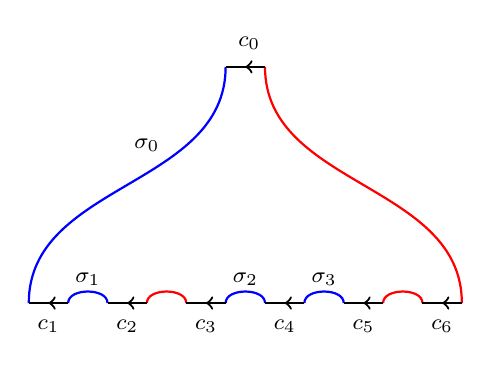
\begin{tikzpicture}[scale=1]
    \tikzset{->-/.style={decoration={ markings,
                mark=at position #1 with {\arrow{>}}},postaction={decorate}}}
    \draw [blue, thick=1.5] (2,3) to[in=90,out=270] (-0.5,0);
    \draw [blue, thick=1.5] (0,0) to[in=90,out=90] (0.5,0);         
    \draw [red, thick=1.5] (1,0) to[in=90,out=90] (1.5,0);         
    \draw [blue, thick=1.5] (2,0) to[in=90,out=90] (2.5,0);         
    \draw [blue, thick=1.5] (3,0) to[in=90,out=90] (3.5,0);         
    \draw [red, thick=1.5] (4,0) to[in=90,out=90] (4.5,0);         
    \draw [red, thick=1.5] (2.5,3) to[in=90,out=270] (5,0);
    \draw [black, thick=1, ->-=.5] (0,0) to (-0.5,0); 
            \draw [black, thick=1, ->-=.5] (1,0) to (0.5,0); 
    \draw [black, thick=1, ->-=.5] (2,0) to (1.5,0); 
    \draw [black, thick=1, ->-=.5] (3,0) to (2.5,0); 
    \draw [black, thick=1, ->-=.5] (4,0) to (3.5,0); 
    \draw [black, thick=1, ->-=.5] (5,0) to (4.5,0); 
    \draw [black, thick=1, ->-=.5] (2.5,3) to (2,3); 

        \node at (2.3, 3.3) {\footnotesize{$c_0$}};
    \node at (-0.25,-0.3) {\footnotesize{$c_1$}}  ;
    \node at (0.75,-0.3) {\footnotesize{$c_2$}}  ;
\node at (1.75,-0.3) {\footnotesize{$c_3$}}  ;
\node at (2.75,-0.3) {\footnotesize{$c_4$}}  ;
\node at (3.75,-0.3) {\footnotesize{$c_5$}}  ;
\node at (4.75,-0.3) {\footnotesize{$c_6$}}  ;

        \node at (1,2) {\footnotesize{$\sigma_0$}}; 
        \node at (0.25, 0.3) {\footnotesize{$\sigma_1$}};
 \node at (2.25, 0.3) {\footnotesize{$\sigma_2$}};
 \node at (3.25, 0.3) {\footnotesize{$\sigma_3$}};
    \end{tikzpicture}
    \caption{Differential in $CE^*$, The word $\sigma_0 c_1 \sigma_1 c_2 c_3 \sigma_2 c_4
    \sigma_3 c_5 c_6$ appears in $dc_0$.}
    \label{diff}
\end{figure}
Consider the moduli space of $J$-holomorphic maps  $u\colon D \to \mathbb{R} \times Y$, where $D$ is a disk with $k+1$ boundary
punctures $z_j \in \partial D = S^1$ that are mutually distinct and $(z_0,z_1,\ldots z_k)$ respects
the counter-clockwise cyclic order of
    $S^1$, and $u$ sends the boundary component $(z_{j-1},z_{j})$  of $S^1          \backslash \{z_0,\ldots,
        z_k \}$ to $\mathbb{R} \times \Lambda$, and is asymptotic to $c_j$ near the puncture at
        $z_j$ for $j=1,\ldots, {k}$ and to $c_0$ near the puncture at $z_0$. The moduli space,
        which is naturally a stratified space with manifold strata that carries a fundamental chain, comes with evaluation maps to $\Omega_{p_v}
        \Lambda_v$ for $v \in \Gamma^{+}$. The image of the fundamental chain determines a word in our chain model of
        $C_{-*}(\Omega_{p_v} \Lambda_v)$. Reading these together with the Reeb chords in order gives
        the differential of $c_0$. 
        
We remark that loop space coefficients were used in the
        context of Lagrangian Floer cohomology before \cite{barcor,Fuk}. See also \cite{abloop},
        \cite{CL} for uses of high-dimensional moduli spaces in Floer theory.  


While $CE^*$ with loop space coefficients is a powerful invariant, it is in general hard to compute
as it involves high-dimensional moduli spaces of disks. As mentioned above, duality in the Legendrian $\Lambda$ will also play a role. More precisely, we define
another DG-algebra $CE^{\ast}_{\parallel}$ related to $CE^*$ via a Morse theoretic version of Adams
cobar construction whose definition involves taking parallel copies of $\Lambda$ but uses only
0-dimensional moduli spaces (see Section \ref{ssec:parallelcopies}). In fact, we prove that the two
DG-algebras are quasi-isomorphic when $\Lambda_{v}$ for $v \in \Gamma^{+}$ are simply-connected. 

\begin{thm} There exists a DG-algebra map 
    \[ CE^* \to CE^*_{\parallel} \]
    which is a quasi-isomorphism when $\Lambda_v$ is simply-connected for all $v \in \Gamma^{+}$.
\end{thm} 

\subsection{Partially wrapped Fukaya categories by surgery}\label{ssec:partwrap} 
Let $\Lambda=\bigsqcup_{v\in\Gamma}\Lambda_{v}$ be a Legendrian submanifold and $\Gamma=\Gamma^{+}\cup\Gamma^{-}$ as above. Furthermore, we use the notation above for co-core disks and write $CE^{\ast}=CE^{\ast}(\Lambda)$.  An important result that is implicit in \cite[Remark 5.9]{BEE} is the following: 

\begin{thm}   \label{srgry}  
    Suppose $\Gamma = \Gamma^{-}$, then there exists a surgery map defined via a holomorphic disk count that gives an 
	$A_\infty$ quasi-isomorphism
    between the wrapped Floer cochain complex    
    $CW^* := \bigoplus_{v,w \in \Gamma^{-} } CW^*(C_v, C_w)$
    and the Legendrian DG-algebra $CE^*$.
\end{thm} 

A complete proof of this result has not yet appeared in the literature. See Appendix
\ref{ssec:CWBEE} for a discussion and a proof sketch. In Appendix \ref{sec:CWnoHam}, one can also find a
construction of wrapped Floer $A_\infty$ algebra which uses only purely holomorphic disks, and a proof that this agrees with the more standard version
defined in \cite{AbouzSeidel} which uses Hamiltonian perturbations. 

One of the main guiding principles for the results in this paper is that Theorem \ref{srgry} remains
true when $\Gamma^{+}$ is non-empty, provided the Lagrangians
$C_v$ are considered as objects of the \emph{partially wrapped} Fukaya category of
$X_\Lambda$, where the non-capped Legendrians $\Lambda_v$ for $v \in \Gamma^{+}$ serve as
\emph{stops} (cf. \cite{sylvan}). The full proof of this result when $\Gamma^+$ is non-empty will appear elsewhere. We give an outline in Appendix \ref{ssec:CWpwrap}.
Here we will use the geometric intuition provided by this viewpoint and our constructions of Legendrian invariants provide a rigorous ``working definition'' of
$CE^*$ even in the case that $\Gamma^{+}$ is non-empty, and also a starting point for the study of
``partially wrapped Fukaya categories'' via Legendrian surgery (extending the scope of \cite{BEE} considerably). For future reference, we state this result as a conjecture:

\begin{conj}\label{conjintro} 
	There exists a surgery map defined via moduli spaces of holomorphic disks which gives an $A_\infty$ quasi-isomorphism between the partially wrapped Floer
    cochain complex $CW^* := \bigoplus_{v,w \in \Gamma} CW^*(C_v,C_w)$ and the DG-algebra 
    $CE^*$. 
\end{conj}

While writing this paper, we learned that Z. Sylvan independently considered a similar conjecture \cite{syltalk} in relation with his theory of partially wrapped Fukaya categories \cite{sylvan}.

\subsection{Augmentations and infinitesimal Fukaya categories}\label{ssec:infinteswrap} 
We keep the notation above and now consider an exact Lagrangian filling $L$ in $X$ of $\Lambda$. Such a filling gives an augmentation 
\[ 
\epsilon_{L} \colon CE^*  \to \k.  
\]
For chords on components $\Lambda_{v}$, $v\in\Gamma^{-}$ this is well known and given by a count of
rigid disks with one positive puncture and boundary on $L_{v}$. For chords on components
$\Lambda_{v}$, $v\in\Gamma^{+}$ the same count composed with the augmentation on $C_{-\ast}(\Omega\Lambda_{v})$ corresponding to the trivial local system gives the augmentation.
This allows us to write 
\[ CE^* = \Omega LC_* \]
for an $A_\infty$ coalgebra $LC_*=LC_{\ast}(\Lambda)$ that we call the \emph{Legendrian $A_\infty$-coalgebra} (which depends on $\epsilon_L$). Here $\Omega$ is the Adams cobar
construction. Writing $LA^{\ast}:= (LC_*)^{\#}$ for the $A_{\infty}$ algebra which is the linear dual of $LC_{\ast}$, the following result recovers the Floer cochain complex of $L$ in $X_\Lambda$.
\begin{thm} \label{generation} There exists an $A_\infty$ quasi-isomorphism between the Floer cochain complex
    in the infinitesimal Fukaya category of $X_\Lambda$,
    $CF^* := CF^*(L_\Lambda)$ 
and the $A_\infty$-module homomorphism of the $\Omega LC^*$-module $\k$,
    $\mathrm{RHom}_{\Omega LC^*} (\k, \k ) \cong LA^*$.
\end{thm}

Note that, by the general properties of bar-cobar constructions (see Section \ref{barcobarsec}), the
algebra $\mathrm{RHom}_{\Omega LC_*} (\k, \k )$ is quasi-isomorphic to the graded
$\k$-dual of the bar construction on the algebra $\Omega LC_*$, which can be computed as 
\[
(\Bar \Cobar LC_*)^\#\cong (LC_*)^\# = LA^*.
\] 

Let us remark that in the case $\Gamma^{+}$ is empty, the $A_\infty$ algebra $LA^*$ is obtained from
the construction in \cite{CEKSW} and \cite{BC}, known as $\mathrm{Aug}_-$ category, by adding a copy of $\k$ making it unital. On the other
hand, in the case $\Gamma^{-}$ is empty, the $A_\infty$ algebra $LA^*$ is related to the
$\mathrm{Aug}_+$ category of \cite{NRSSZ}. In the setting of microlocal sheaves, a related result
was obtained by Nadler \cite[Theorem 1.6]{nadler}.


\subsection{Duality between partially wrapped and infinitesimal Fukaya categories}\label{ssec:connections} 

We study duality in the setting of the two categories described above: the partially wrapped Fukaya category and the infinitesimal Fukaya category of
$X_\Lambda$ (after surgery), or equivalently, the augmented DG-algebra $\Omega LC^*$ and the
augmented $A_\infty$ algebra $LA^*$ (before surgery). 

As we have seen in Theorem \ref{generation}, the augmented
DG-algebra $\Omega LC_*$ determines the augmented (unital) $A_\infty$ algebra
$CF^*$. Now, a natural question is to what extent the quasi-isomorphism type of the $A_\infty$ algebra
$CF^*$ determines the quasi-isomorphism type of the augmented Legendrian DG-algebra $\Omega LC_*$. 

We emphasize here the phrase ``quasi-isomorphism type'': even though it is possible
to construct chain models of the $A_\infty$ algebra  $LA^*$ (which is $A_\infty$ quasi-isomorphic to
$CF^*$) and the DG-algebra $\Omega LC_*$ by counting ``the same'' holomorphic disks interpreted in
different ways, the two algebras are considered with respect to different
equivalence relations, and the resulting equivalence classes can be very different. In particular, it is \emph{not} generally true that $\mathfrak{f}\colon \C \to \mathscr{D}$ being a
quasi-isomorphism of $A_\infty$-coalgebras implies that $\Omega
\mathfrak{f}\colon \Omega \C \to \Omega \mathscr{D}$ is a quasi-isomorphism. 

We will study this question by (geometrically) constructing a \emph{twisting cochain} (see
Section \ref{twisting}): 
\[ \t \colon LC_* \to (\Bar CF^*)^\#,  \] 
where $\Bar$ stands for the bar construction and $\#$ is the graded $\k$-dual.
This twisting cochain induces a map of DG-algebras:
\[ \Omega LC_* \to \mathrm{RHom}_{CF^*}( \k, \k), \]
which is a quasi-isomorphism if and only if $\t$ is a \emph{Koszul} twisting cochain. For
example, we will prove the following result. 

\begin{thm} Suppose that $LC_*$ is a locally finite, simply-connected $\k$-bimodule, then
    the natural map $\Omega LC_* \to \mathrm{RHom}_{CF^*}(\k, \k)$ is a quasi-isomorphism.
\end{thm}

This is an instance of \emph{Koszul duality} between the $A_\infty$ algebras $\Omega LC_*$ and
$CF^*$. This duality has many useful implications. For example, it implies an isomorphism between Hochschild cohomologies: 
\[
HH^*(\Omega LC_*, \Omega LC_*) \cong HH^*(CF^*, CF^*).
\]
When $\Gamma^+ = \varnothing$, an isomorphism defined via a surgery map \cite{BEE} was described between \emph{symplectic cohomology}, $SH^{\ast}=SH^*(X_{\Lambda})$, and the Hochschild cohomology $HH^*(\Omega LC_*, \Omega LC_*)$. Therefore, when duality holds, we obtain a more economical way of computing $SH^*$. 

In the case of cotangent bundles $T^{\ast}M$ of simply-connected manifolds $M$, this recovers a classical result due to
Jones \cite{jones}, which gives:
\[ H_{n-*}(\mathcal{L} M) \cong HH^*(C_{-*}(\Omega M), C_{-*}(\Omega M)) \cong HH^*(CF^*(M),
CF^*(M)), \] 
where $M$ is simply-connected manifold of dimension $n$ and $\mathcal{L} M$ denotes the free loop space of $M$.

In Section \ref{ssec:applications}, we give several concrete examples where the duality holds beyond the
case of cotangent bundles. For example, the duality holds for plumbings of simply-connected cotangent bundles
according to an arbitrary plumbing tree, see Theorem \ref{plumbs}. 

In another direction, combining duality and Floer cohomology with local coefficients, we establish the following result for relatively spin exact Lagrangian fillings $L\subset X$ with vanishing Maslov class of a Legendrian submanifold $\Lambda\subset Y$. 

\begin{thm}
	Let $\Gamma=\Gamma^{-}$ and assume that $SH^*(X)=0$ and that $\Lambda$ is simply-connected. If $CE^{\ast}(\Lambda)$ is supported in degrees $<0$, then $L$ is simply connected. Moreover, if $\Lambda$ is a sphere then $CE^{\ast}(\Lambda)$ is isomorphic to $C_{-\ast}(\Omega \overline{L})$, where $\overline{L}=L\cup_{\Lambda} D$, for a disk $D$ with boundary $\partial D=\Lambda$.
\end{thm}  
 

In general, duality between $\Omega LC_{\ast}$ and $CF^{\ast}$ does not hold (as can be seen for example by looking at
cotangent bundles of non-simply connected manifolds or, letting $\Lambda$ be the
standard Legendrian trefoil knot in $S^3$ filled by a punctured torus). However, there are cases
when duality holds even if $LC_*$ is not simply-connected, for instance because of the existence of
an auxiliary weight grading, see \cite{EtLe} or for an example in the 1-dimensional case see
\cite{LePol}. It is a very interesting open question to find a geometric characterization of when duality holds. 


\begin{rem}
As is well known, general constructions of Legendrian and Lagrangian holomorphic curve invariants
    require the use of so-called abstract perturbations. For our main invariant $CE^{\ast}$,   
all moduli spaces used can be shown to be transverse by classical techniques (see Theorem (\ref{thm:mdlitv})) except for the rigid holomorphic planes in $X_\Lambda$ with a single positive end that are used to anchor the disks in the terminology of \cite{BEE}.  (These are also relevant for defining the wrapped Floer cochain complex $CW^*$ without Hamiltonian perturbations and for constructing the surgery map). In symplectic field theory similar transversality problems are dealt with by appealing to virtual perturbation techniques, see e.g. \cite{FOOO,Hofer,Pardon,HondaBao}. 
Here we will not work out the details of this but merely assume such a perturbation scheme has been fixed. Our results are independent of the particular choice.

We also point out that our construction of $CE^{\ast}$ applies without reference to virtual techniques in a number of interesting cases where splitting off of holomorphic planes can be ruled  out for topological reasons. For example, if there are no contractible Reeb orbits, e.g. for $X=\R^{2n}$.  


%For our purposes, we find such assumptions unnatural and obscuring
%    (though, they can usually be arranged to hold pre-surgery, for ex. for $X=\mathbb{R}^{2n}$), and will continue in the general framework by
%    appealing to virtual techniques precisely to address this issue.
\end{rem}




\subsection{An example -- the Hopf Link}\label{ssec:Hopflink}

In this section, we study the example of the Hopf link in order to illustrate our results in a simple and computable example. Some of the algebraic constructions used here are
explained in detail only later, see Section \ref{algebra}. 

\begin{figure}[h!]
    \centering
    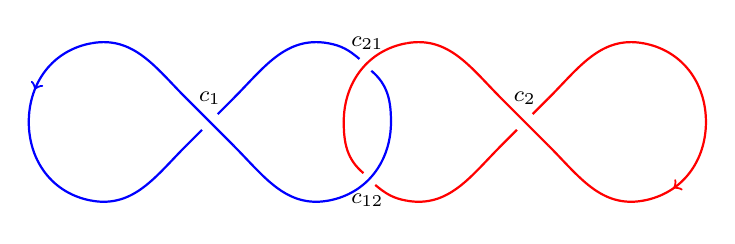
\begin{tikzpicture}[scale=1]
        %  \tikzset{->-/.style={decoration={ markings,
         %             mark=at position #1 with {\arrow[scale=2,>=stealth]{>}}},
          %            postaction={decorate}}}


    \tikzset{->-/.style={decoration={ markings,
                mark=at position #1 with {\arrow{>}}},postaction={decorate}}}
            
\draw [blue, thick=1.5, ->-=.7] (-1.5,1) to[in=90,out=190] (-2.3,0);
    \draw [blue, thick=1.5] (-1.5,1) to[in=135,out=10] (-0.3,0.3);         
    \draw [blue, thick=1.5]  (-1.5,-1)to[in=270,out=170] (-2.3,0);
    \draw [blue, thick=1.5] (-1.5,-1)to[in=225,out=350] (-0.3,-0.3)  ;
    
    \draw [blue, thick=1.5] (1.5,1) to[in=45,out=170] (0.3,0.3);         
    
    \draw [blue, thick=1.5]  (1.5,-1)to[in=270,out=10] (2.3,0);
    \draw [blue, thick=1.5] (1.5,1) to[in=140,out=350] (1.9,0.8);
    \draw [blue, thick=1.5] (2.05,0.65) to[in=90,out=320] (2.3,0);
 
    
    \draw [blue, thick=1.5] (1.5,-1)to[in=315,out=190] (0.3,-0.3)  ;

    \draw [blue, thick=1.5] (-0.3,0.3) to (0.3,-0.3);
    \draw [blue, thick=1.5] (-0.3,-0.3) to (-0.1,-0.1);
    \draw [blue, thick=1.5] (0.1,0.1) to (0.3,0.3);

    \draw [red, thick=1.5] (2.5,1) to[in=90,out=190] (1.7,0);

    \draw [red, thick=1.5] (2.5,-1) to[in=320,out=170] (2.1,-0.8);
    \draw [red, thick=1.5] (1.95,-0.65) to[in=270,out=140] (1.7,0);


    \draw [red, thick=1.5] (2.5,1) to[in=135,out=10] (3.7,0.3);         
    \draw [red, thick=1.5] (2.5,-1)to[in=225,out=350] (3.7,-0.3)  ;
    
    \draw [red, thick=1.5] (5.5,1) to[in=90,out=350] (6.3,0);
    \draw [red, thick=1.5] (5.5,1) to[in=45,out=170] (4.3,0.3);         
    \draw [red, thick=1.5, ->-=.7]  (6.3,0)to[in=10,out=270] (5.5,-1);
    \draw [red, thick=1.5] (5.5,-1)to[in=315,out=190] (4.3,-0.3)  ;

    \draw [red, thick=1.5] (3.7,0.3) to (4.3,-0.3);
    \draw [red, thick=1.5] (3.7,-0.3) to (3.9,-0.1);
    \draw [red, thick=1.5] (4.1,0.1) to (4.3,0.3);

    \node at (0,0.3) {\footnotesize{$c_1$}}; 
        \node at (2,1) {\footnotesize{$c_{21}$}}; 
        \node at (2,-1) {\footnotesize{$c_{12}$}}; 
    \node at (4,0.3) {\footnotesize{$c_2$}}; 

    \end{tikzpicture}
    \caption{Hopf link when both $\Gamma^{+}$ and $\Gamma^{-}$ are
    non-empty, the blue component lies in $\Gamma^{+}$ and the red in $\Gamma^{-}$.}
    \label{hopf}
\end{figure}

Let $\Lambda \subset S^3$ be the standard Legendrian Hopf link. We work over $\k =
\mathbb{K} e_1 \oplus \mathbb{K} e_2$ and with the Lagrangian filling $L$ given by two disks in $D^4$ that intersect transversely in a single point.
We choose the partition $\Lambda = \Lambda^+ \cup \Lambda^-$. This means that after attaching a Weinstein 2-handle to $\Lambda^{-}$ and $T^{\ast}(S^{1}\times[0,\infty))$ to $\Lambda^{+}$, we obtain the symplectic manifold $X_{\Lambda}$ with Lagrangian skeleton 
\[ L_\Lambda = S^2 \cup T_{\mathrm{pt}}^* S^2 \subset T^{\ast} S^{2}, \]
or in the terminology of \cite{sylvan}, $X_{\Lambda}$ is $T^{\ast}S^{2}$ with wrapping stopped by a Legendrian fiber sphere.   
The DG-algebra $CE^{\ast}=CE^*(\Lambda)$ of $\Lambda$ has coefficients in 
\[C_{-*}(\Omega \Lambda^+) e_1 \oplus \mathbb{K} e_2 \cong \K[t,t^{-1}] e_1 \oplus \K e_2. \]
A free model for $\K[t,t^{-1}]$ is given by the tensor algebra $\K\langle s_1,
t_1, k_1, l_1, u_1 \rangle$ with $|s_1|=|t_1|=0$, $|k_1|=|l_1|=-1$, $|u_1|=-2$ and the differential  
\begin{align*}
    dk_1 &= e_1 - s_1 t_1 \\
    dl_1 &= e_1 - t_1 s_1 \\
    du_1 &= k_1 s_1 - s_1 l_1 
\end{align*}
The subscripts indicate that as $\k$-module generators
$s_1, t_1, k_1, l_1, u_1$ are annihilated by the idempotent $e_2$. 
Next, incorporating the Reeb chords, with notation as in Figure \ref{hopf}, we get the free algebra 
\[  \k \langle c_{12} , c_{21} , c_{1}, c_{2},
s_1, t_1, k_1, l_1, u_1 \rangle \] 
with gradings\[|u_1|=-2, |c_{1}|=|c_{2}| = |k_1|= |l_1|=  -1,\ |c_{12}|=|c_{21}|=|s_1|=|t_1|=0  \] and differential:
\begin{align*} 
    dc_1 &= e_1 + s_1 + c_{12}c_{21}, \\
    dc_2 &= c_{21} c_{12}, \\
    dk_1 &= e_1 - s_1 t_1, \\
    dl_1 &= e_1 - t_1 s_1, \\
    du_1 &= k_1 s_1 - s_1 l_1. 
\end{align*}
The only augmentation to $\k$ is given by $\epsilon(s_1) = \epsilon(t_1) = -e_1$, and
$\epsilon(c_1) = \epsilon(c_2) = \epsilon(c_{12})
=\epsilon(c_{21})=\epsilon(k_1)= \epsilon(l_1)= \epsilon(u_1) = 0$. After change of
variables, $s_1 \to s_1 - e_1$ and $t_1 \to t_1 - e_1$, we obtain the free algebra 
\[ \k \langle c_{12} , c_{21} , c_{1}, c_{2},
s_1, t_1, k_1, l_1, u_1 \rangle \] 
with non-zero differential on generators: 
\begin{equation}
\begin{aligned} 
    dc_1 &= s_1 + c_{12}c_{21}, \\
    dc_2 &= c_{21} c_{12}, \\
    dk_1 &= s_1 +t_1 - s_1 t_1, \\
    dl_1 &= s_1 +t_1  - t_1 s_1, \\
    du_1 &= l_1 -k_1 + k_1 s_1 - s_1 l_1. 
\end{aligned}
\end{equation}
On the other hand, we can compute the Floer cochains $CF^{\ast}=CF^{\ast}(L_{\Lambda})$ of $L_\Lambda$ as 
\[ CF^* = \k \oplus \mathbb{K} a_{12} \oplus \K a_{21} \oplus \K a_2, \
|a_{2}|=2,\ |a_{12}|=|a_{21}|=1 \] 
The cohomology level
computation follows easily from the geometric picture and general properties of Floer cohomology:  $L_\Lambda$ is a union of a disk $D^2$ and
a sphere $S^2$ that intersect transversely in one point and we have
\begin{align*}
    HF^*(D^2,D^2) &= \K e_1 \\
    HF^*(S^2,S^2) &= \K e_2 \oplus \K a_2 \\
    HF^*(D^2,S^2) &= \K a_{12} \\
    HF^*(S^2,D^2) &= \K a_{21} 
\end{align*}
The only non-trivial product that does not involve idempotents is given by $\m_2(a_{12},a_{21}) = a_2$. For degree reasons, the only possible non-trivial higher products are:
\[ \m_{2k} (a_{12},a_{21}, \ldots, a_{12},a_{21}) = ca_2  \text{\ for some  } k >1 \text{ and } c
\in \K.\]
It turns out that one can take $c=0$ for all $k>1$. Indeed, assuming that the $A_\infty$ structure
is strictly unital (which can be arranged up to quasi-isomorphism), consider the $A_\infty$ relation that involves the term
\[ \m_2( m_{2k}(a_{12},a_{21},\ldots,a_{12},a_{21}), e_2). \]
By induction on $k>1$, this term has to vanish, which implies
$m_{2k}(a_{12},a_{21},\ldots,a_{12},a_{21})$ has to vanish for all $k>1$. Let us confirm this by
using the quasi-isomorphism:
\[ CF^*  \cong \mathrm{RHom}_{CE^*}(\k,\k).\] 
We introduce the counital $A_\infty$-coalgebra
\[ LC_* = \k \oplus \mathbb{K} c_{12} \oplus \K
c_{21} \oplus \K c_{1} \oplus \K c_{2} \oplus \K s_1 \oplus \K t_1 \oplus \K k_1 \oplus \K l_1
\oplus \K u_1 \] 
with $|u_1|=-3, |c_{1}|=|c_{2}| = |k_1|= |l_1|=  -2,\ |c_{12}|=|c_{21}|=|s_1|=|t_1|=-1$ 
for which $\Delta_{i}=0$ except for $i=1$ or 2 where there are the following non-zero terms:  
\begin{align*} 
    \Delta_1 (c_1) &= s_1, \\
    \Delta_1 (k_1) &= s_1 + t_1, \\
    \Delta_1 (l_1) &= s_1 + t_1, \\
    \Delta_1 (u_1) &= l_1 - k_1.
\end{align*}
Write $\Delta_2 (x) = 1 \otimes_\k x + x \otimes_\k 1 +
\overline{\Delta}_2(x)$. Then
\begin{align*}
    \overline{\Delta}_2(c_1) &= c_{12} c_{21}, \\
    \overline{\Delta}_2(c_{2}) &= c_{21} c_{12}, \\ 
    \overline{\Delta}_2(k_1) &= - s_1 t_1, \\ 
    \overline{\Delta}_2(l_1) &= - t_1 s_1, \\
    \overline{\Delta}_2(u_1) &=  k_1 s_1 - s_1 l_1,
\end{align*} 
where the $A_\infty$ coalgebra operations on $LC_* $ is defined so that $\Omega LC_*$ is isomorphic to $CE^*$. Thus, $\mathrm{RHom}_{CE^*}(\k,\k)$ can be computed as the graded dual of $LC_*$ which is the $A_\infty$ algebra: 
\[ LA^*= \k \oplus \K c_{12}^\vee \oplus \K 
c_{21}^\vee \oplus \K c_{1}^\vee \oplus \K c_{2}^\vee \oplus \K s_1^\vee \oplus \K t_1^\vee \oplus
\K k_1^\vee \oplus \K l_1^\vee \oplus \K u_1^\vee,  \]
with gradings  
\[ 
|u_1^\vee|=3, |c_{1}^\vee|=|c_{2}^\vee| = |k_1^\vee|=|l_1^\vee| =  2,\
|c_{12}^\vee|=|c_{21}^\vee|=|s_1^\vee|=|t_1^\vee|=1, 
\]
where $c^{\vee}$ is the linear dual of the generator $c$ of $LC_{\ast}$.
The differential is  \[ \m_1(s_1^\vee) = c_1^\vee + k_1^\vee + l_1^\vee,
\m_1(t_1^\vee)=k_1^\vee + l_1^\vee, \m_1 (k_1^\vee) = -u_1, \m_1(l_1^\vee) = u_1, \] and the
products that do not involve
idempotents are  
\begin{align*} &\m_2(c_{12}^\vee,c_{21}^\vee) = c_2^\vee, \m_2(c_{21}^\vee, c_{12}^\vee) = c_1^\vee ,
    \m_2(t_1^\vee,s_1^\vee) = -k_1^\vee,\\ &\m_2(s_1^\vee,t_1^\vee) = -l_1^\vee,  \m_2(k_1^\vee,s_1^\vee) =
u_1^\vee, \m_2(s_1^\vee,l_1^\vee) = -u_1^\vee.   
\end{align*} 

All the higher
products vanish. 
We claim that that this $A_\infty$ algebra is quasi-isomorphic to the algebra
\[  \k \oplus \mathbb{K} a_{12} \oplus \K a_{21} \oplus \K a_2, \
|a_{2}|=2,\ |a_{12}|=|a_{21}|=1  \]
with the only non-trivial product (not involving idempotents) given by \[ \m_2(a_{12},a_{21}) =a_2.\]  
Indeed, it is easy to show that the map defined by:
\[ c^\vee_{12} \to a_{12}, c_{21}^\vee \to a_{21}, c_2^\vee \to a_2 , \text{\ and \ } c_1^\vee, s_1^\vee,
t_1^\vee, k_1^\vee, l_1^\vee, u_1^\vee\to 0 \]
is a DG-algebra (hence also $A_\infty$-algebra) map, which induces an isomorphism at the level of
cohomology. 

Dually, we can construct a $DG$-algebra map 
\[ CE^* \to \mathrm{RHom}_{CF^*}(\k,\k). \]
The Floer cochain complex $CF^*$ has a unique augmentation given by projection to $\k$ and we compute 
\[ \mathrm{RHom}_{CF^*}(\k,\k) \cong \Cobar CF_*, \]
where $CF_*$ is the coalgebra dual to $CF^{\ast}$. This is the free coalgebra
\[  \k \langle a^\vee_{12} , a^\vee_{21} , a^\vee_{2} \rangle \] 
with $|a_{12}^\vee|=|a_{21}^\vee|=0$ and $|a^\vee_{2}|=-1$ and the only non-trivial differential not involving counits is
\[ \Delta_{2}(a^\vee_{2}) = a_{21}^\vee a_{12}^\vee. \] 
We have a twisting cochain 
\[ \t\colon LC_* \to \Omega CF_* \]
given by  \begin{align*}
    \t (c_2) &= a^\vee_2,\ \t (c_{12}) = a^\vee_{12},\ \t (c_{21}) = a^\vee_{21},\\
    \t(c_1) &=0,\ \t (s_1) = -a_{12}^\vee a_{21}^\vee ,\ \t (t_1) = a_{12}^\vee a_{21}^\vee,\ \\  \t
    (l_1) &= \t(k_1)=  a_{12}^\vee
    a_2^\vee a_{21}^\vee, \t(u_1) = a_{12}^\vee a_2^\vee a_2^\vee a_{21}^\vee.
\end{align*}
This means that $\t$ satisfies the following equations:
\begin{align*} 
    d\t(c_1) &= \t(s_1) + \t(c_{12}) \t(c_{21}), \\
    d\t(c_2) &= \t(c_{21}) \t(c_{12}), \\
    d\t(k_1) &= \t(s_1) + \t(t_1) - \t(s_1) \t(t_1), \\
    d\t(l_1) &= \t(s_1) + \t(t_1) - \t(t_1) \t(s_1), \\
    d\t(u_1) &= \t(l_1) -\t(k_1) + \t(k_1) \t(s_1) - \t(s_1) \t(l_1).  
\end{align*}
Hence, it induces a DG-algebra map 
\[  \Omega LC_*  \to \Omega  CF_*. \]
We have not checked whether this is a quasi-isomorphism, or equivalently whether $\t$ is a
\emph{Koszul} twisting cochain. Note, however, the DG-algebra map $\Omega CF_* \to \Omega LC_* $ defined by
\[ a_2^\vee \to c_2, a_{12}^\vee \to c_{12}, a_{21}^\vee  \to c_{21}, \]
shows that $\t$ is a retraction, and $\Omega CF_* $ is a retract of $\Omega LC_*$.


\vspace{.5cm}

\noindent
{\bf Acknowledgments.} T.E. is supported by the Knut and Alice Wallenberg Foundation and by the
Swedish Research Council. Y.L. is supported in part by the Royal Society (URF) and the NSF grant
DMS-1509141. Both authors would like to thank the Mittag-Leffler institute for hospitality and
excellent working conditions. We also thank Lenny Ng for providing the example in Section
\ref{lenny}, and Zack Sylvan for his interest. 

\section{Algebraic preliminary}
\label{algebra} 


In this section, we review the homological algebra we use in our study of various invariants
associated to Legendrian submanifolds and their Lagrangian fillings. Most of this material is well
established, see \cite{L-H} and also
\cite{proute}, \cite{Posit}, \cite{herscovich}, \cite{LV}, \cite{LPWZ}. Note though that our sign conventions follow \cite{seidelbook}, see Remark \ref{rem:Seidelsign}. 

\subsection{$A_\infty$ algebras and coalgebras}

In this section we will discuss the basic algebraic objects we use. These are modules over a ground ring $\k$ of the following form.  
Fix a coefficient field $\mathbb{K}$ (of arbitrary characteristic) and let $\k$ be a semi-simple ring of the form:
\[ 
\k = \oplus_{v\in\Gamma} \,\mathbb{K} e_v 
\]
where $e_v^2= e_v$ and $e_v e_w =0$ for $v \neq w$, and where the index set $\Gamma$ is finite.

We will use $\Z$-graded $\k$-bimodules. If $M= \bigoplus_i M^{i}$ is such a module then we call $M$ \emph{connected} if $M^0 \cong \k$ and
either $M^i =0$ for all $i>0$, or $M^{i}=0$ for all $i<0$, and we call $M$ \emph{simply-connected} if, in addition, in the former case $M^{-1}=0$ and in the latter $M^{1}=0$. Further, we say that $M$ is \emph{locally finite} if each $M^i$ is finitely generated as a $\k$-bimodule.  

%With this convention, the coalgebra $C_{-*}(L)$ is the graded dual of the algebra $C^*(L)$. We use 
%We write this as: $C_{-*}(L) = C^*(L)^\#$. 
We have the usual shifting and tensor product operations on modules. If $M = \bigoplus_{i} M^{i} $ is a graded $\k$-bimodule and $s$ is an integer then we let the corresponding shifted module $M[s]=\bigoplus_{i}M[s]^{i}$ be the module with graded components  
\[ 
M[s]^{i} = M^{i+s}. 
\]
If $N=\bigoplus_{i} N^{i}$ is another graded $\k$-bimodule then
$M\otimes_{\k}N=\bigoplus_{k}\left(M\otimes_{\k}N\right)^{k}$ is naturally a graded $\k$-bimodule with
\[ \left(M\otimes_{\k}N\right)^{k}=\bigoplus_{i+j=k}M^{i}\otimes_{\k} N^{j}.
\]
For iterated tensor products we write 
\[  
M^{\otimes_{\k}r}=\underbrace{M\otimes_{\k}\ldots \otimes_{\k} M}_{r}.
\]

Our modules will often have further structure as $\Z$-graded $A_\infty$-algebras and $A_\infty$-coalgebras over $\k$, see Sections \ref{ssec:Ainftyalg} and \ref{ssec:Ainftycoalg}. The modules are then in particular chain complexes with a differential and we will use \emph{cohomological} grading throughout. That is, the differential \emph{increases} the grading by 1. For
example, if $L$ is a topological space then its cohomology complex $C^*(L)$ is supported in
non-negative grading, while the homology complex $C_{-*}(L)$ is supported in non-positive degrees.
To be consistent with this, we denote the grading as a subscript (resp. superscript) when the underlying chain
complex has a coalgebra (resp. algebra) structure. 


\subsubsection{$A_{\infty}$-algebras}\label{ssec:Ainftyalg} An \emph{$A_\infty$-algebra} over $\k$
is a $\Z$-graded $\k$-module $\A$ with a collection of grading preserving $\k$-linear maps \[ \m_i
\colon \A^{\otimes_\k i } \to \A [2-i],  \] for all integers $i \geq 1$, that satisfies the
$A_\infty$-relations: \begin{equation} \label{ainf} \sum_{i,j} (-1)^{|a_1|+\ldots + |a_j|-j}
\m_{d-i+1}\left(a_d,\ldots, a_{j+i+1},\m_i(a_{j+i},\ldots, a_{j+1}), a_j,\ldots, a_1\right) = 0,
\end{equation} for all $d$. 

\begin{rem}\label{rem:Seidelsign}
	We follow the sign conventions of \cite{seidelbook}. Note that
	even though, $\m_i$ is written on the left of $(a_{j+i},\ldots, a_{j+1})$, the sign
	convention is so that $\m_i$ acts from the right. To be consistent, we will insist that all our
	operators act on the right independently of how they are written. This convention and the usual
	Koszul sign exchange rule determine the signs that appear in our formulas. 
\end{rem}




A \emph{DG-algebra} over $\k$ is an $A_\infty$-algebra $\A$ such that $\m_i =0$ for $i \geq 3$. In this
case, we call the first two operations the \emph{differential} and the \emph{product}, respectively, and use the following adjustments to obtain an (ordinary) differential graded algebra: 
\begin{equation} \label{left} 
    d a = (-1)^{|a|} \m_1(a) \quad \text{ and } \quad a_2 a_1 = (-1)^{|a_1|} \m_2(a_2,a_1). 
\end{equation}
In particular, the product is then associative and the graded Leibniz rule for $d$ holds:
\begin{equation} \label{Leib} 
    d(a_2 a_1) = (d a_2) a_1 + (-1)^{|a_2|} a_2 (da_1). 
\end{equation}
An \emph{$A_{\infty}$-map} $\e\colon\A\to\B$ between $A_{\infty}$-algebras $\A$ and $\B$ over $\k$, with operations $\m_i$ and $\n_{i}$, $i\ge 1$, respectively, is a collection of $\k$-linear grading preserving maps 
\[ 
\e_i \colon \A^{\otimes_\k i } \to \B [1-i],  
\]
$i\ge 1$, that satisfies the relations
\begin{align*} 
\sum_{i,j} (-1)^{|a_1|+\ldots + |a_j|-j} 
\e_{d-i+1}\left(a_d,\ldots, a_{j+i+1},\m_i(a_{j+i},\ldots, a_{j+1}), a_j,\ldots, a_1\right) \ &+ \\ 
\sum_{\begin{smallmatrix}
1\le j\le d, \\
0<i_{1}<i_{2}<\dots<i_{j}<d
\end{smallmatrix}}  
\n_{j}\left(\e_{d-i_{j}}(a_d,\ldots,a_{d-i_{j}}),\ldots,\e_{i_2-i_1}(a_{i_2},\ldots,a_{i_1+1}), \e_{i_1}(a_{i_1},\ldots, a_{1})\right)&= 0. 
\end{align*}

An $A_\infty$-map $\e \colon \A \to \B$ is called an \emph{$A_\infty$-quasi isomorphism} if the map on
cohomology $H^*(\A) \to H^*(\B)$ induced by $\e^1$ is an isomorphism.

We say that an $A_{\infty}$-algebra $\A$ is \emph{strictly unital} if there is
an element $1_\A \in\A$ such that $\m_1(1_\A)=0$, $\m_2(1_\A,a)=\m_{2}(a,1_\A)=a$ for any $a\in\A$, and such that
$\m_{i}$, $i > 2$ annihilates any monomial containing $1_\A$ as a factor.  

An \emph{augmentation} of a strictly unital $A_\infty$-algebra is an $A_\infty$-map $\epsilon \colon \A \to \k$,
where $\k$ is considered as a strictly unital $A_\infty$-algebra in degree 0 with trivial
differential and higher $A_\infty$-products, and such
that $\epsilon_1 (1_\A)=1_\k$, $\epsilon_i$ for $i>1$ annihilates any monomial containing $1_\A$.
An augmentation is called $\emph{strict}$ if $\epsilon_{i}=0$ for $i>1$. The category of
augmented, strictly unital $A_\infty$ algebras is equivalent to the category of strictly
augmented, strictly unital $A_\infty$ algebras (see \cite[Section 7.2]{Posit}). 

\subsubsection{$A_{\infty}$-coalgebras}\label{ssec:Ainftycoalg}
An \emph{$A_\infty$-coalgebra} $\C$ over $\k$ is a $\Z$-graded $\k$-module with a collection of
$\k$-linear grading preserving maps:
\[ 
\Delta_i\colon \C \to \C^{\otimes_\k i}[2-i],
\]
for all integers $i \geq 1$, with the following properties. The maps satisfy the co-$A_\infty$-relations:
\begin{equation} \label{coainf} 
\sum_{i=1}^d \sum_{j=0}^{d-i} ( \id^{\otimes_\k (d-i-j)} \otimes_\k \Delta_i \otimes_\k
\id^{\otimes_\k\, j} ) \Delta_{d-i+1} = 0, 
\end{equation}
where,  
\begin{align*} 
    \id^{\otimes_\k (d-i-j)}&\otimes_\k \Delta_i\otimes_\k \id^{\otimes_\k j}\,(c_{d-i+1},\ldots, c_{1}) =\\
    &(-1)^{|c_{1}| +\ldots+ |c_{j}|-j} (c_{d-i+1} , \ldots, c_{j+2})\otimes_\k \Delta_i(c_{j+1}) \otimes_\k (c_{j} ,
    \ldots , c_{1})\\
    & \in \C^{\otimes_\k (d-i-j)} \otimes_\k \C^{\otimes_\k i} \otimes_\k
    \C^{\otimes_\k j}. 
\end{align*}
Furthermore, the degree 1 map
\[ 
\C[-1] \to \prod_{i=1}^\infty \C[-1]^{\otimes_\k i}, 
\]
with $i^{\rm th}$ component equal to $\Delta_i$, factorizes through the natural inclusion
\[ 
\bigoplus_{i=1}^\infty \C[-1]^{\otimes_\k i} \to \prod_{i=1}^\infty \C[-1]^{\otimes_\k i}, 
\]
of the direct sum into the direct product.    
    
A \emph{DG-coalgebra} over $\k$ is an $A_\infty$-coalgebra such that $\Delta_i=0$ for $i\geq 3$.
In this case, we call the first two operations the \emph{differential} and the \emph{coproduct},
respectively, and use the following adjustments to obtain an (ordinary) differential
graded coalgebra:
\begin{equation} \label{coleft}  
    \theta c = (-1)^{|c|} \Delta_1(c) \quad \text{ and } \quad \Delta(c) = 
    \sum (-1)^{|c_{(2)}|} c_{(1)} \otimes_\k c_{(2)}, 
\end{equation}
where we write $\Delta_2(c) = \sum c_{(1)} \otimes_\k c_{(2)}$. 

In particular, the coproduct is coassociative (i.e. $(\Delta \otimes_\k \id)\circ \Delta = (\id
\otimes_\k \Delta) \circ \Delta$) and the graded co-Leibniz rule holds:
\begin{equation} \label{coLeib}
\Delta \theta(c) = \sum (-1)^{|c_{(1)}|} c_{(1)} \otimes_{\k} \theta(c_{(2)}) + \theta(c_{(1)})
\otimes_\k c_{(2)}. 
\end{equation}

A DG-coalgebra $\C$ is called \emph{conilpotent} (also called
\emph{cocomplete})  if for any $c\in \C$,
there exists an $n \geq 2$ such that $c$ is in the kernel of the iterated comultiplication map defined recursively by $\Delta^{(2)}=\Delta$ and 
$\Delta^{(n)}=(\id^{\otimes_\k (n-2)} \otimes_\k \Delta) \circ \Delta^{(n-1)}$, for $n>2$.


An \emph{$A_{\infty}$-comap} $\mathfrak{f} \colon\C\to\D$ between $A_{\infty}$-coalgebras $\C$ and $\D$ over
$\k$, with operations $\Delta_i$ and $\Theta_{i}$, $i\ge 1$, respectively, is a collection of $\k$-linear grading preserving maps 
\[ 
    \mathfrak{f}_i \colon \C \to \D^{\otimes_\k i}[1-i], 
\]
$i\ge 1$, that satisfies the relations:
\begin{align*} 
    \sum_{i=1}^{d} \sum_{j=0}^{d-i} \left(\id^{\otimes_\k (d-i-j)} \otimes_\k \Theta_i \otimes_\k
\id^{\otimes_\k j} \right) \mathfrak{f}_{d-i+1}  \ &+ \\ 
\sum_{\begin{smallmatrix}
1\le j\le d, \\
0<i_{1}<i_{2}<\dots<i_{j}<d
\end{smallmatrix}}  
\left( \mathfrak{f}_{d-i_j} \otimes_\k \cdots \otimes_\k \mathfrak{f}_{i_2-i_1} \otimes_\k \mathfrak{f}_{i_1} \right) \Delta_j   &= 0. 
\end{align*}
where, 
\begin{align*} 
    \id^{\otimes_\k (d-i-j)}\otimes_\k &\Theta_i\otimes_\k \id^{\otimes_\k j}\,(d_{d-i+1},\ldots, d_{1}) =\\
    &(-1)^{|d_{1}|+\ldots+|d_{j}|-j} (d_{d-i+1} , \ldots, d_{j+2})\otimes_\k \Theta_i(d_{j+1}) \otimes_\k (d_{j} ,
    \ldots , d_{1})\\
    & \in \D^{\otimes_\k (d-i-j)} \otimes_\k \D^{\otimes_\k i} \otimes_\k
    \D^{\otimes_\k j}. 
\end{align*}

Furthermore, the degree 0 map 
\[ \C[-1] \to \prod_{i=1}^\infty \D[-1]^{\otimes_\k i} \]
with $i^{th}$ component equal to $\mathfrak{f}_i$, factorizes through the natural inclusion:
\begin{equation} \label{factor} 
\bigoplus_{i=1}^\infty \D[-1]^{\otimes_\k i} \to \prod_{i=1}^\infty \D[-1]^{\otimes_\k i}, 
\end{equation}
of the direct sum into the direct product.    

An $A_\infty$-comap $\mathfrak{f} \colon \C \to \D$ is called an \emph{$A_\infty$-quasi isomorphism} if the map on
cohomology $H^*(\C) \to H^*(\D)$ induced by $\mathfrak{f}^1$ is an isomorphism.

We say that an $A_\infty$-coalgebra is \emph{strictly counital} if there exists a $\k$-linear map
$\epsilon\colon \C \to \k$ such that $(\epsilon \otimes \id) \Delta_2 = (\id
\otimes \epsilon) \Delta_2 = \id$ and $(\id^{\otimes_\k (i-j)} \otimes_\k \epsilon \otimes_\k
\id^{\otimes_\k\, j-1}) \Delta_i =0$ for all $i \neq 2$ and $j$. 


A \emph{coaugmentation} of a strictly counital $A_\infty$-coalgebra $\C$ is an $A_\infty$-comap $\eta \colon\k \to
\C$, where $\k$ is considered as a vector space in degree 0 with the trivial
$A_\infty$-coalgebra structure, such that $\epsilon \eta_1 = 1_\k$ and 
$(\id^{\otimes_\k (i-j)} \otimes_\k \epsilon \otimes_\k \id^{\otimes_\k\, j-1}) \eta_i =0$ for all
$i>1$ and $j$. The coaugmentation is called \emph{strict} if $\eta_i=0$ for $i \geq 2$. 

\subsubsection{Graded dual}\label{ssec:gradeddual}
We next discuss the graded dual of a graded $\k$-module. Since we are working over a noncommutative
ring $\k$, there are two $\k$-linear duals (cf. \cite{bgs}). 

If $\A$ is a graded $\k$-module, $\A=\bigoplus_{i}\A_{i}$, then the $\emph{graded duals}$
$\A^{\#}=\bigoplus_{i}(\A^{\#})_{i}$ and $^{\#}\!\A =\bigoplus_{i}(^{\#}\!\A)_{i}$ are defined as
follows. The graded components $(\A^{\#})_{i}$ of $\A^{\#}$ are left $\k$-module maps:
\[ 
\mathrm{hom}_{\k-}(\A_{-i},\k),
\] 
and the $\k$-bimodule structure on $\A^{\#}$ is given as follows: if $e_v,e_w\in\k$, $a\in(\A^{\#})_{i}$, and $c\in \A_{-i}$, then
\begin{equation} \label{leftkbimodule} 
(e_v \cdot a \cdot e_w) (c) = a(ce_v ) e_w. 
\end{equation}
The graded components $(^{\#}\!\A)_{i}$ of $^\#\!\A$ in degree $i$ are right $\k$-module maps,
which we write as:
\[ 
\mathrm{hom}_{-\k}(\A_{-i},\k),
\] 
and the $\k$-bimodule structure is given by: 
if $e_v,e_w\in\k$, $a\in(^{\#}\!\A)_{i}$, and $c\in \A_{-i}$, then
\begin{equation} \label{rightkbimodule}
(e_v \cdot a \cdot e_w) (c) = e_v a(e_w c). 
\end{equation}
Both canonical maps $\A \to \!^\#(\A^\#)$ and $\A \to (^\#\!\A)^\#$ are $\k$-bimodule maps, which are isomorphisms if $\A$ is locally finite.

If $V_1,V_2,\ldots, V_n$ are $\k$-bimodules, there is a natural map 
\[V_n^\# \otimes_\k  V_{n-1}^\# \otimes_\k \cdots \otimes_\k V_1^\# \to (V_1 \otimes_\k V_2 \otimes_\k \cdots \otimes_\k V_n)^\# \]
given  by:
\begin{equation}\label{composition} 
(a_n \otimes a_{n-1} \otimes \ldots \otimes a_1) (c_1 \otimes c_2 \otimes \ldots\otimes c_n ) :=
    a_1(c_1 a_2(c_2 \ldots a_n(c_n) \ldots)).  
\end{equation}
Similarly, there is a natural map 
\[^\# V_n \otimes_\k\!^\# V_{n-1} \otimes_\k \cdots \otimes_\k \!^\# V_1 \to \!^\#(V_1 \otimes_\k V_2
\otimes_\k \cdots \otimes_\k V_n), \]
given  by:
\begin{equation}\label{composition2} 
    (a_n \otimes a_{n-1} \otimes \ldots \otimes a_1) (c_1 \otimes c_2 \otimes \ldots\otimes c_n ) := a_n (\ldots a_2(a_1(c_1)c_2)\ldots c_n).  
\end{equation}

These give the graded duals $\C^\#$ and $\!^\#\C$ of a coaugmented $A_\infty$-coalgebra $\C$ the structure of augmented $A_\infty$-algebras with structure maps defined by:
\begin{equation}\label{dualainf} \m_i(a_i,\ldots,a_1) (c) := (-1)^{|c|} (a_i \otimes \ldots \otimes a_1)
\Delta_i (c). \end{equation}
Note that to get a non-zero product, we must have $|\m_i(a_i,\ldots,a_1)|=|c|$, hence the sign $(-1)^{|c|}$ equals the sign $(-1)^{|a_1|+\ldots+|a_i|-i}$.

In general, there is no natural way of equipping the graded dual of an augmented $A_\infty$-algebra with an $A_\infty$-coalgebra structure. However, if the grading on $\A$ is locally finite (i.e.
$\A_i$ are finitely generated as $\k$-bimodules), then it follows that
\begin{align*}
    \A^\# \otimes_{\k} \A^\# \otimes_\k \cdots \otimes_\k \A^{\#} &\cong (\A         \otimes_\k \A
    \otimes_\k
\cdots \otimes_\k \A)^\#, \\
    \!^\#\A\! \otimes_{\k} \!^\#\!\A \otimes_\k \cdots \otimes_\k \!^{\#}\!\A &\cong \!^\# (\A         \otimes_\k \A \otimes_\k \cdots \otimes_\k \A).
\end{align*}  Therefore, the graded duals $\A^\#$ and $^\#\!\A$ of an augmented
        $A_\infty$-algebra $\A$ with locally finite grading are naturally coaugmented $A_\infty$-coalgebras. 

\subsubsection{Twisting cochains}
\label{twisting} 

Let $(\mathscr{C}, \Delta_{\bullet})$ be an $A_\infty$-coalgebra and let $(\mathscr{A},
\m_1, \m_2)$ be a DG-algebra. A \emph{twisting cochain} is a $\k$-linear map $\mathfrak{t}\colon
\mathscr{C} \to \mathscr{A}$ of degree 1 that satisfies:
\begin{equation}\label{eq:twcochain}
    \m_1 \circ \mathfrak{t} - \mathfrak{t} \circ \Delta_1 + \sum_{d \geq 2} (-1)^d \m_2^{(d)}
\circ \mathfrak{t}^{\otimes_\k d} \circ \Delta_d = 0, 
\end{equation}
where $\m_2^{(2)} := \m_2$, and $\m_2^{(d)} := \m_2\circ
(\mathrm{Id}_\mathscr{A} \otimes_\k \m_2^{(d-1)})$. Note that for
$c \in \mathscr{C}$, $\Delta_i(c) \neq 0$ for only finitely many $i$, and hence the potentially infinite sum in \eqref{eq:twcochain} is actually finite when it acts on $c$.

If the coalgebra $\C$ is coaugmented by $\eta\colon \k \to \C$ and the algebra $\A$ is augmented
$\epsilon\colon \A \to \k$, we require in addition that its  twisting cochains $\t$ are compatible in the sense that  \begin{equation}
\t \circ \eta = \epsilon \circ \t =0.
\end{equation}
We denote the set of twisting cochains from $\C$ to $\A$ by $\mathrm{Tw}(\C,\A)$. 


Let $\t\in\mathrm{Tw}(\C,\A)$ be a twisting cochain. Consider the twisted tensor product $\A
\otimes^\mathfrak{t}_\k \C$ as a chain complex with 
differential $d^{\mathfrak{t}}\colon \A\otimes^\mathfrak{t}_\k \C\to\A\otimes^\mathfrak{t}_\k \C$ defined as follows,
\begin{equation}\label{koszulcomplex} 
d^\mathfrak{t} = \m_1 \otimes_\k \mathrm{Id}_\C + \mathrm{Id}_\A \otimes_\k \Delta_1 +
\sum_{d \geq 2} (\m_2^{(d)} \otimes \mathrm{Id}_\C) \circ (\mathrm{Id}_\A \otimes_\k
\mathfrak{t}^{\otimes_{\k} d-1}
\otimes_\k \mathrm{Id}_\C ) \circ (\mathrm{Id}_\A \otimes_\k \Delta_{d}). 
\end{equation}
Here the differential squares to zero, $d^\mathfrak{t} \circ d^\mathfrak{t}=0$, since
$\mathfrak{t}$ satisfies \eqref{eq:twcochain}. This complex is the \emph{Koszul complex}
associated with $\t$. It is called acyclic if the projection to $\k$ is a quasi-isomorphism. 

Note that one also has an analogous complex of the form $\C
\otimes_{\k}^{\t} \A$.  

The $\mathbb{K}$-vector space of $\k$-bimodule morphisms $\hom_{\k-\k}(\C,\A)$ carries an $A_\infty$-algebra
structure with operations $\mathfrak{n}_d$, $d\ge 1$ given by
\[ \mathfrak{n}_1 (t) = \m_1 \circ t + (-1)^{|t|} t \circ \Delta_1 \]
and 
\[ 
\mathfrak{n}_d (t_d, t_{d-1}, \ldots, t_1) = (-1)^{d(|t_d|+\ldots+|t_1|)} \m_2^{(d)} \circ (t_d \otimes t_{d-1} \otimes
\ldots \otimes t_1) \circ \Delta_d ,  \ \ d\geq 2. 
\] 
where the composition $(t_d \otimes t_{d-1} \otimes \ldots \otimes t_1) \circ \Delta_d$ is defined
component-wise. Thus, if $\Delta_d(c)= c_d \otimes \ldots \otimes c_1$, then 
\[ (t_d \otimes_\k t_{d-1} \otimes_\k \ldots, t_1)\Delta_d(c) = (-1)^\dagger \t_d(c_d)\otimes_\k
\t_{d-1}(c_{d-1}) \ldots  \otimes_\k t_1(c_1), \] 
where $\dagger = \sum_{j=2}^d \sum_{i=1}^{j-1} |c_i||t_j|$.
In this setting, a twisting cochain $\mathfrak{t}\colon \C \to \A$ corresponds to a solution of the Maurer-Cartan equation:
\begin{equation}\label{eq:MCeq} 
\sum_{i \geq 1} \mathfrak{n}_i (\mathfrak{t}, \mathfrak{t}, \ldots, \mathfrak{t}) =0. 
\end{equation} 
(As before, this sum is effectively finite since for any $c \in \C$, $\Delta_i(c)\neq 0$ only for finitely many $i$.). 

In particular, a twisting cochain $\mathfrak{t}\colon \mathscr{C} \to \mathscr{A}$ defines a twisted $A_\infty$-structure on $\hom_\k (\C, \A)$, with operations $\mathfrak{n}^{\mathfrak{t}}_{d}$ given by
\[ 
\n^\mathfrak{t}_d (t_d,t_{d-1},\ldots, t_1) = \sum_{l_i \geq 0} \n_{d+l_0+l_1+\ldots+l_d}
(\overbrace{\mathfrak{t},\ldots, \mathfrak{t}}^{l_d},
t_d, \overbrace{\mathfrak{t},\ldots, \mathfrak{t}}^{l_{d-1}}, t_{d-1},\;\ldots\;, 
t_1,\overbrace{\mathfrak{t},\ldots, \mathfrak{t}}^{l_0}).  
\]
We will denote this twisted $A_\infty$-structure $\hom^\mathfrak{t}_{\k}(\C,\A)$.

There are direct analogs of the above construction if we instead consider a DG-coalgebra $(\mathscr{C}, \Delta_1, \Delta_2)$ and an $A_\infty$-algebra $\mathscr{A}$ with operations $\m_i$. 
The module $\hom_{\k-\k} (\mathscr{C},\mathscr{A})$ has the structure of an $A_\infty$-algebra with operations $\mathfrak{n}_d$ given by:
\[ 
\mathfrak{n}_1 (t) = \m_1 \circ t + (-1)^{|t|} t \circ \Delta_1 
\]
and 
\[ 
\mathfrak{n}_d (t_d, t_{d-1}, \ldots, t_1) = \m_d \circ (t_d \otimes t_{d-1} \otimes
\ldots \otimes t_1) \circ \Delta_2^{(d)} ,  \ \ d\geq 2. 
\] 
To make sense of the twisting cochain equation \eqref{eq:MCeq}, one needs to make additional assumptions to ensure the convergence of the infinite sum. This holds, for example, if $\C$ is conilpotent.

We remark that if both $\C$ and $\A$ are $A_\infty$-(co)algebras, then defining a twisting
cochain is a more complicated matter (cf. \cite[Introduction]{proute}). We will not need this here.

\subsection{Bar-cobar duality for $A_\infty$-(co)algebras}
In this section we first introduce the bar and cobar constructions and then discuss basic relations between them.


\subsubsection{Bar and cobar constructions} 
\label{barcobarsec}
Let $(\A, \{\m_j\}_{j \geq 1})$ be a strictly unital $A_\infty$-algebra with a strict
augmentation $\epsilon\colon \A \to \k$. Define the \emph{augmentation ideal} $\Abar =\mathrm{ker}
(\epsilon)$. Note that if we are given a non-unital $A_\infty$-algebra $\Abar$, then we can turn it into a strictly unital
$A_\infty$ algebra $\A := \k \oplus \Abar$ with an augmentation given by projection to $\k$. 

We next recall the construction of the (reduced) \emph{bar construction} $\Bar \A$. For any augmented $A_\infty$-algebra $\A$, $\Bar \A$ is a coaugmented conilpotent DG-coalgebra. As a coaugmented coalgebra $\Bar \A$ is defined as
\[ 
\Bar \A = \k \oplus \Abar [1] \oplus \Abar [1]^{\otimes_\k 2} \oplus \ldots,  
\]
where $[1]$ denotes the downwards shift by 1. We write a typical monomial using Eilenberg and
Maclane's notation: \[ [a_d|a_{d-1}|\ldots |a_1] = sa_d \otimes_\k sa_{d-1} \otimes_\k \ldots
\otimes_\k sa_1, \]
where for $a \in \Abar$, $sa \in \Abar[1]$ denotes the corresponding element in $\Abar[1]$ with degree shifted down by 1. 

The differential $b\colon \Bar \A \to \Bar \A$ is defined to vanish on $\k\subset\A$, $b_{|\k}=0$, and as follows on monomials:
\[ 
b([a_d|a_{d-1}|\ldots|a_1]) = \sum_{i,j} (-1)^{|a_1|+\ldots+|a_j|-j}
[a_d|\ldots|a_{j+i+1}|\m_i(a_{j+i},\ldots,a_{j+1})|a_{j}|\ldots|a_1], 
\]
where strictness of the augmentation ensures that $\m_i(a_{j+i},\ldots, a_{j+1}) \in \Abar[1]$ for
$(a_{j+i},\ldots, a_{j+1}) \in \Abar[1]^{i}$. (If the augmentation is not strict, one applies a quasi-isomorphism of $\A$ to make it strict.) 

The coproduct $\Delta_2 \colon \Bar \A \to \Bar \A \otimes_\k \Bar \A $ is defined by
\[ 
\Delta_2 ([a_d|a_{d-1}|\ldots |a_1]) = \sum_{i=0}^d (-1)^{|a_i|+\ldots+|a_1|-i}  [a_d|a_{d-1}|\ldots|a_{i+1}] \otimes_\k [a_{i}|
    a_{i-1}|\ldots | a_1]. 
\]
The slightly unusual sign $(-1)^{|a_i|+\ldots+|a_1|-i}$ appears as a consequence of the following two facts:
\begin{itemize}
\item[$(\mathrm{i})$]
    The equation $b^2=0$ is equivalent to the $A_\infty$-relations \eqref{ainf} for
$(\m_i)_{i\geq 1}$, 
\item[$(\mathrm{ii})$]
The pair $(b,\Delta_2)$ satisfies the co-$A_\infty$ relations
\eqref{coainf}. 
\end{itemize}
Redefining $(b,\Delta_2)$ to $(\theta, \Delta) $
using \eqref{coleft} removes the sign in $\Delta_2$, and $(\theta, \Delta)$ becomes a (usual)
coassociative DG-coalgebra, where the co-Leibniz rule \eqref{coLeib} holds. The coaugmentation $\eta\colon \k \to \Bar \A$ is defined by letting $\eta_{1}$ be the inclusion of $\k$ and $\eta_{i}=0$ for $i>0$.

There is an increasing, exhaustive, and bounded below (hence, complete Hausdorff) filtration on the complex  $\Bar \A$:
\[ 
\k = \F^{0}\Bar\A \subset \F^1 \Bar\A \subset \cdots \subset \Bar \A, 
\]
where
\[ 
\F^p \Bar \A := \k \oplus \Abar[1] \oplus \cdots \oplus \Abar[1]^{\otimes_\k p}.  
\]
This induces the \emph{word-length spectral sequence} with
\[ E_1^{p,q} = H^{p+q} (\F^{p} \Bar \A / \F^{p-1} \Bar \A) \]
converging strongly to
\[ E_\infty^{p,q} = \F^{p} H^{p+q} (\Bar \A) / \F^{p-1} H^{p+q} (\Bar \A) \]
by the classical convergence theorem (\cite[Theorem 5.5.1]{weibel}). It can be proved using this spectral sequence that an $A_\infty$ map $\e \colon \A \to \B$ is a
quasi-isomorphism if and only if the naturally induced DG-coalgebra map $\Bar\e \colon \Bar \A \to \Bar \B$ is a quasi-isomorphism, see \cite[Proposition 2.2.3]{LV}. 

There is a universal twisting cochain $\t_\A \colon \Bar \A \to \A$ which is non-zero only on
$\Abar[1] \subset \Bar \A$ and is given by the inclusion map $\Abar[1] \to \A$. The twisting cochain $\t_\A$ gives rise to a free $\A$-bimodule resolution of $\A$ obtained as a
twisted tensor product
\[ \A \otimes_{\k}^{\t_\A} \Bar \A \otimes_{\k}^{\t_\A} \A, \]
with the differential $d$ given by the following formula:
\begin{align} \label{bimodulediff} 
	d&=\m_1 \otimes_\k \mathrm{Id}_{\Bar \A} \otimes_\k \mathrm{Id}_{\A}  + \mathrm{Id}_{\A}
    \otimes_\k b \otimes_\k \mathrm{Id}_\A +  \mathrm{Id}_\A \otimes_\k \mathrm{Id}_{\Bar \A}
    \otimes_\k \m_1 \\\notag
    &+ \left(\sum_{d \geq 2 }
(\m_d \otimes_{\k} \mathrm{Id}_{\Bar \A}) \circ (\mathrm{Id}_\A \otimes_\k \t^{\otimes_\k {d-1}} \otimes_\k \mathrm{Id}_{\Bar
\A})  \circ
(\mathrm{Id}_{\A} \otimes_\k
    \Delta_2^{(d)}) \right) \otimes_{k} \mathrm{Id}_\A \\\notag 
    &+ \mathrm{Id}_\A \otimes_k \left(\sum_{d \geq 2 }
    (\mathrm{Id}_{\Bar \A} \otimes_\k \m_d) \circ (\mathrm{Id}_{\Bar \A} \otimes_\k \t^{\otimes_\k {d-1}} \otimes_\k \mathrm{Id}_{\A})  \circ
    (\Delta_2^{(d)} \otimes_\k \mathrm{Id}_{\A} ) \right).
\end{align}

This can be used to compute Hochschild homology and cohomology of $\A$ with coefficients in
an $\A$-bimodule $\mathscr{M}$. 

Consider instead a strictly counital $A_\infty$-coalgebra $\C$ with operations $\Delta_i$ and
with a strict coaugmentation $\eta\colon \k \to \C$. Let $\Cbar = \mathrm{coker}(\eta)$ be the coaugmentation ideal. We next recall the \emph{cobar construction} which associates a DG-algebra $\Omega \C$ to $\C$.  As an augmented algebra $\Omega \C$ is:
    \[ \Omega \C = \k \oplus \Cbar [-1] \oplus \Cbar [-1]^{\otimes_\k 2} \oplus \ldots .\]
As before, we write a typical monomial as \[ [c_d|c_{d-1}|\ldots |c_1] = s^{-1} c_d \otimes_\k
s^{-1} c_{d-1} \otimes_\k \ldots
\otimes_\k s^{-1} c_1, \]
where for $c \in \Cbar$, $s^{-1} c \in \Cbar[-1]$ denotes the corresponding element in $\Cbar[-1]$ with degree shifted up by 1. The differential $\m_{1}$ on $\Omega \C$ vanishes on $\k$, $\m_{1}|_{\k}=0$, and acts as follows on monomials:
\[ \m_1 ([c_m|\ldots |c_1]) = \sum_{i,j} (-1)^{|c_{1}|+\ldots+|c_i|-i}
    [c_m|\ldots|c_{i+2}|\Delta_j(c_{i+1})|c_{i}|\ldots |c_1]. \]
Here, by abuse of notation, we write $\Delta_j$ for the induced coproduct $\Cbar[-1] \to \Cbar[-1]^{\otimes j}$.

    The product $\m_{2} \colon \Omega \C \otimes \Omega \C \to \Omega \C$ is given by:
    \[ \m_2 ([c_m|\ldots |c_{i+1}], [c_{i}|\ldots|c_1]) =
    (-1)^{|c_{1}|+\ldots |c_i|-i} [c_m|\ldots|c_{i+1}|c_{i}|\ldots|c_1] \]
The slightly unusual sign $(-1)^{|c_{1}|+\ldots+|c_i|-i}$ appears as a consequence of the following two facts:
\begin{itemize}
\item[$(\mathrm{i})$]	
The equation $\m_1^2=0$ is equivalent to co-$A_\infty$ relations \eqref{coainf} for
$(\Delta_j)_{j\geq 1}$. 
\item[$(\mathrm{ii})$]
The pair $(\m_1,\m_2)$ satisfies the $A_\infty$ relations \eqref{ainf}. 
\end{itemize} 
Redefining $(\m_1,\m_2)$ to $(d, \cdot) $
using \eqref{left} removes the sign in $\m_2$, and $(d, \cdot)$ becomes a (usual) associative
DG-algebra, where Leibniz rule \eqref{Leib} holds. The augmentation $\epsilon\colon \Omega \C \to \k$ is given by letting $\epsilon_1$ to be the projection
to $\k$ and $\epsilon_i =0$ for $i>0$. 

There is a decreasing, exhaustive, bounded above filtration on the complex     $\Omega \C$:
    \[ \Omega \C = \F^{0}\Omega \C \supset \F^1 \Omega \C \supset \ldots,\]
given by
\[ \F^p \Omega \C := \Cbar[-1]^{\otimes_\k p} \oplus \Cbar[-1]^{\otimes_\k (p+1) }\oplus \ldots. 
\]
This gives the \emph{word length spectral sequence} with
\[ E_1^{p,q} = H^{p+q} (\F^{p} \Omega \C / \F^{p+1} \Omega \C). \]
Unlike the case of the word length filtration on the bar construction, for the cobar construction, in general, convergence may fail. Thus, we introduce
completions. We define the \emph{completed cobar construction} to be: 
\[ \widehat{\Omega} \C = \varprojlim_s (\Omega \C)/ (\F^{s} \Omega \C) \]
The length filtration on $\Omega \C$ induces a filtration $\widehat{\F}$ on $\widehat{\Omega}
\C$ defined by:
\[ \widehat{\F}^p \widehat{\Omega} \C  = \varprojlim_s (\F^{p} \Omega \C) / (\F^{s} \Omega \C) \]
which is decreasing, exhaustive, bounded above and complete Hausdorff. The spectral sequence associated to the filtration $\widehat{\F}$ on $\widehat{\Omega}
\C$
is isomorphic to the length spectral sequence associated with the filtration $\widehat{\F}$ on
$\Omega \C$ and converges conditionally to $H^*(\widehat{\Omega} \C)$ (see \cite[Theorem
9.2]{boardman}). It converges strongly to $H^*(\widehat{\Omega} \C)$ if the spectral sequence is
regular, i.e., only finitely many of the differentials $d_{r}^{p,q}$ are nonzero for each $p$ and $q$
(see \cite[Theorem 7.1]{boardman}). This holds, for example, if $\Omega \C$ is locally finite.  


We say that $\Omega\C$ is complete if the natural map $\Omega \C \to \widehat{\Omega}
\C$ is a quasi-isomorphism. For example, it is easy to see that this is the case if $\C$ is locally
finite and simply-connected. 

If $\mathfrak{f}\colon \C \to \D$ is an $A_\infty$-comap which is a quasi-isomorphism of $A_\infty$-coalgebras and if $\Omega\C$ is complete then $\Omega \mathfrak{f}$ is a quasi-isomorphism. (This follows from \cite[Theorem 7.4]{EM}, see also \cite[Theorem 5.5.11]{weibel}).
The condition that $\Omega \C$ is complete is necessary and is related to the completeness of the
word length filtration. A counter-example when the completeness assumption is dropped can be found in \cite[Section 2.4.1]{LV}. 

There is a universal twisting cochain $\t^\C\colon \C \to \Omega \C$ given by the composition of
canonical projection $\C \to \Cbar[-1]$ and the canonical inclusion $\Cbar[-1] \to \Omega \C$.


\subsubsection{Bar-cobar adjunction}\label{ssec:barcobaradj}
Suppose that $\C$ is a coaugmented $A_\infty$-coalgebra and $\A$ is an augmented DG-algebra, then we have a canonical
bijection 
\begin{equation}\label{bij1}  
\hom_{DG} (\Omega \C, \A) \to \mathrm{Tw}(\C,\A),
\end{equation} 
given by $\phi \mapsto \phi \circ \t^\C$.
Similarly, if $\C$ is a coaugmented conilpotent DG-coalgebra and $\A$ is an augmented $A_\infty$-algebra, then we have a canonical
bijection 
\begin{equation}\label{bij2} 
\hom_{coDG} (\C, \Bar \A) \to \mathrm{Tw}(\C,\A), 
\end{equation}
given by $\phi \mapsto \t_\A \circ \phi$ (see Lemme 3.17 \cite{proute}).

Therefore, when $\C$ is a coaugmented conilpotent DG-coalgebra, and $\A$ is an augmented DG-algebra, we have the bar-cobar adjunction: 
\[ \hom_{DG}( \Omega \C, \A) \cong \hom_{coDG}(\C, \Bar \A). \]

Notice, in particular, that the natural DG-maps
 \begin{equation} \label{barcobar} \Omega \Bar \A \to \A \ \ , \ \ \C \to \Bar \Omega \C \end{equation}
     are quasi-isomorphisms for any DG-algebra $\A$ and conilpotent DG-coalgebra $\C$
     (see \cite[Section 6.10]{Posit}). It is also
 true that for any $A_\infty$-algebra $\A$, the $A_\infty$ algebra map \[ \A \to \Omega \Bar \A\] given
 by the adjunction map $\Bar \A \to \Bar \Omega \Bar \A$ is an
 $A_\infty$-quasi-isomorphism (see
 \cite[Lemme 2.3.4.3]{L-H}). Note that any $A_\infty$-quasi-isomorphism is invertible up to
 homotopy (\cite[Corollary 1.4]{seidelbook}).

Similarly, for any $A_\infty$-coalgebra $\C$, the $A_\infty$-comap 
 \[ \Bar \Cobar \C \to \C \]
given by the adjunction map $\Omega \Bar \Omega \C \to \C$ is an $A_\infty$ quasi-isomorphism. 

However, an $A_\infty$ quasi-isomorphism for a general $A_\infty$-coalgebra is not usually a convenient notion,
since as we remarked above a quasi-isomorphism of $A_\infty$ coalgebras between $\C$ and $\C'$ does not
necessarily induce a quasi-isomorphism of DG-algebras $\Cobar \C$ and $\Cobar \C'$.

For this reason, one considers the category of \emph{conilpotent} $A_\infty$ coalgebras. Let $\C$ be
a coaugmented $A_\infty$-coalgebra generated over $\k$ by variables $(c_i)_{i\in I}$ with $I$ some countable index set, such that there exists a total ordering 
    \[ c_{\sigma(1)} < c_{\sigma(2)} < \ldots \]
    where $\sigma\colon I \to I$ is a bijection. This produces an increasing  filtration 
    \[ \mathcal{F}^0 =\k \subset \mathcal{F}^1 \subset \cdots \subset \Omega \C \] 
    by setting $\mathcal{F}^p = \k \langle c_{\sigma(1)},\ldots, c_{\sigma(p)} \rangle$.
    Suppose that the structure maps $(\Delta_i)_{i\geq 1}$ are compatible with this filtration, in
    the sense that, $\Delta_i(c_{\sigma(p)}) \subset \mathcal{F}^{p-1}$ for all $i$ and $p$. Then we
    call $\C$ a conilpotent $A_\infty$ coalgebra. (More generally, a homotopy retract of such
    $A_\infty$ coalgebras are called conilpotent, cf. \cite[Sections 6.10 and 9]{Posit}. This notion is called \emph{finite type} in \cite{Kontsevich}.). 
    Given two such $A_\infty$ coalgebras $\C$
    and $\C'$, one considers filtered $A_\infty$-comaps between them. 
In the case of a conilpotent DG-coalgebra $\C$ there exists an increasing filtration on $\Omega \C$
given by the subalgebras $\mathrm{Ker}(\Delta^{(n)})$ that plays the same role (see \cite[Lemme
1.3.2.3]{L-H}). 

We next state the following elementary lemma for later convenience.

\begin{lem} \label{dualbar} Let $\A$ be an augmented $A_\infty$-algebra, such that the $\k$-bimodule
    structure on $\A$ and $\Bar \A$ are locally finite, then there are quasi-isomorphisms of
    augmented DG-algebras: \begin{align*} \Omega(\A^\#) \to (\Bar \A)^\#  \text{\ \ \ and\ \ \ }
        \Omega(^\#\A) \to \!^\#(\Bar \A). 
    \end{align*}  \end{lem}

Note that the assumption is satisfied when $\A$ is simply-connected. We shall also consider the
case when $\A$ is assumed to be connected, then we have:
\begin{lem} \label{dualbar0} Let $\A = \bigoplus_{i} \A^{i}$ be a connected, locally finite
    $\k$-bimodule equipped with an augmented $A_\infty$-algebra structure, then there are maps of
    DG-algebras
    \[ \Omega(\A^\#) \to (\Bar \A)^\# \text{\ \ \ and \ \ \ }\Omega(^\#\!\A) \to \!^\#(\Bar \A),
    \]  
which become quasi-isomorphisms  after completion:
    \[ \widehat{\Omega}(\A^\#) \to (\Bar \A)^\# \text{\ \ \ and \ \ \ } \widehat{\Omega}(^\#\!\A) \to \!^\#(\Bar \A).  \] 
\end{lem}

\subsection{Koszul duality} 
    \label{algkoszul} 

Suppose $\C$ is a coaugmented conilpotent $A_\infty$-coalgebra and $\A$ is an augmented DG-algebra, via the bijection \eqref{bij1}, any twisting cochain $\t \in \mathrm{Tw}(\C,\A)$ is of the form $\t = \phi \circ
    \t^\C$ for some unique $\phi \in \hom_{DG}(\Omega\C,\A)$. 
    Similarly, if $\C$ is a coaugmented DG-algebra and $\A$ is an augmented $A_\infty$-algebra, any twisting cochain $\t \in \mathrm{Tw}(\C,\A)$ is of the form $\t = \t_\A \circ \phi$
    for some $\phi \in \hom_{coDG}(\C, \Bar \A)$. 

\begin{defi}\label{ktc}    
In either case above we call $\t$ a \emph{Koszul twisting cochain} if $\phi$ is a quasi-isomorphism, and we denote the set of Koszul twisting cochains by $\mathrm{Kos}(\C,\A)$. 
\end{defi}

The terminology of Koszul twisting cochains is taken from \cite{LV}. They are also called $\emph{acyclic twisting cochains}$ in other sources (cf. \cite{L-H}, \cite{Posit}). This terminology is due to the well known fact that, under various locally finiteness assumptions, a twisting cochain $\t$ is Koszul if and only if the Koszul complex (\ref{koszulcomplex}) associated $\t$ is acyclic (cf. \cite[Appendix A]{Posit}).

Informally, if $\t \in \mathrm{Kos}(\C, \A)$ then, depending on whether we write
    $\t=\phi\circ\t^{\C}$ or $\t=\t_{\A}\circ\phi$, either $\A$ can be used in place of $\Omega \C$
    or $\C$ can be used in place of $\Bar \A$
in various resolutions. This, in turn, may lead to smaller complexes to compute with. For example,
    one can compute Hochschild homology and cohomology of $\A$ and $\Omega \C$ using the
    $\A$-bimodule resolution of $\A$ given by the complex:
    \[ \A \otimes_{\k}^{\t} \C \otimes_{\k}^{\t} \A \] 
    with the differential as in \eqref{bimodulediff}, see \cite{herscovich}.

Suppose that $\A$ is an $A_\infty$-algebra with an augmentation
$\epsilon\colon \A\to \k$. The augmentation $\epsilon$ makes $\k$ into a left $\A$-module or          equivalently a
right $\A^{op}$-module. 

\begin{defi} The \emph{Koszul dual} of an augmented $A_\infty$-algebra $\A$ is the DG-algebra of left $\A$-module maps     from $\k$ to
    itself:
        \[ E(\A) := \rhom_{\A} (\k,\k). \]
    \end{defi}
(Here, the $\k$-bimodule structure on $E(\A)$ is given by \eqref{leftkbimodule} since $\k$ is
viewed as a left $\k$-module induced from its structure as a left $\A$-module. If instead, we have
an augmentation of $\A^{op}$, then we view $\k$ as a right $\A$-module, and the
$\k$-bimodule structure on $\rhom_{\A}(\k,\k)$ would be given by \eqref{rightkbimodule} ). 

    Recall that for a unital $A_\infty$-algebra $\A$ over a field $\mathbb{K}$ (or a semisimple ring such
    as $\k$) any $A_\infty$-module is both $h$-projective and $h$-injective, that is, if $M$ is an
    $A_\infty$-module over $\A$ and $N$ is an acyclic $A_\infty$ module over $\A$, then the
    complexes $\rhom_{\A}(M,N)$ and $\rhom_{\A}(N,M)$ are acyclic \cite[Lemma 1.16]{seidelbook}. Hence, the DG-algebra
    $\rhom_{\A}(\k,\k)$ can be computed as the $A_\infty$-module homomorphisms from     $\k$ to
    itself. (More generally, this holds if $\A$ is $h$-projective as a complex of $\k$-
    modules, which implies that $\k$ is $h$-projective as an $A_\infty$-module over $\A$.) Therefore, we have the following.

\begin{prop} If $\A$ (resp. $\A^{op}$) is an augmented unital $A_\infty$-algebra then
    \[ \rhom_{\A}(\k,\k) \cong
    (\Bar\A)^\# \ \ \ (\text{resp.} \ \  \!^\#(\Bar \A) \  ). \]    
\end{prop}
\begin{proof} Recall that $\A \otimes_\k \Bar\A$ is quasi-isomorphic to $\k$ as an $\A$-  module. Hence,
        by the hom-tensor adjunction, we have $\rhom_{\A} (\A \otimes_\k \Bar\A , \k) \cong
        \rhom_{\k} (\Bar\A,
            \k )$. Since $\A$ is $h$-projective as a complex of $\k$-modules, so is $\Bar\A$, hence
            the latter
                is computed by $(\Bar\A)^\#$.
            \end{proof}
The cohomology is a graded algebra:     \[ \mathrm{Ext}_{\A}(\k,\k) := H^*          (\rhom_{\A}(\k,\k)) \cong
H^*((\Bar\A)^\#). \]
Dually, we also have the derived tensor product $\k \widehat{\otimes}_\A \k$, which can be computed
by the complex $\Bar\A$. The cohomology is a graded coalgebra:
\[ \mathrm{Tor}_{\A}(\k,\k) := H^*(\k \widehat{\otimes}_\A \k) \cong H^*(\Bar\A). \]
In particular, note that if $\k$ is a field, we have that $\mathrm{Ext}_{\A}(\k,\k) \cong
(\mathrm{Tor}_{\A}(\k,\k))^\#$ by the universal coefficient theorem.


\begin{rem} If $\A$ is a {\bf commutative} algebra (or more generally an $E_2$-algebra), then $\mathrm{Tor}_{\A}(\k,   \k)$ also has a graded
algebra structure defined via:
\[ \mathrm{Tor}_{\A}(\k,\k) \otimes \mathrm{Tor}_{\A}(\k, \k) \to
\mathrm{Tor}_{\A \otimes \A }(\k \otimes \k, \k \otimes \k) \to                     \mathrm{Tor}_{\A}(\k,\k) \]
induced by the algebra map $\A \otimes \A \to \A$ (which exists since $\A$ is       commutative). This should not be confused with the natural coalgebra structure      above.
\end{rem}

Note that $\A$ itself can be viewed as a left $\A$-module and the map
$\epsilon \colon \A \to \k$ is a map of left $\A$-modules, hence it induces a map of DG- algebras:
\[ \tilde{\epsilon}\colon \rhom_{\A}(\k,\k)^{op} \to \rhom_{\A}(\A,\k), \]
which can in turn be viewed as an augmentation of $E(\A)^{op} = \rhom_{\A}(\k,      \k)^{op}$ since
$\rhom_{\A}(\A,\k)$ can again be
identified with $\k$ as it is the Yoneda image of $\k$ as an $\A$-module. Hence,    $\k$ can be viewed
as a right $E(\A)$-module.
\begin{defi}
The double-dual of
$\A$ is defined to be $E(E(\A)):=\rhom_{E(\A)}(\k,\k)$.
\end{defi}

There is a natural map from $\A$ to its double-dual:
\[ \Phi\colon \A \to \rhom_{E(\A)}(\k,\k) \]
defined via viewing the right $E(\A)$-module $\k$ as $\rhom_{\A}(\A,\k)$ and acting on the left by $\A
\cong\rhom_{\A}(\A,\A)$.

\begin{defi} We say that $\A$ and $E(\A)$ are Koszul dual if $\Phi\colon \A \to \rhom_{E(\A)}(\k,\k)$ is a quasi-isomorphism.
\end{defi}

One standard situation when Koszul duality holds is the following:

\begin{thm} \label{doubledual} Suppose $\C = \bigoplus_{i \leq 0} \C^i$ is a locally finite, simply-connected $\k$-bimodule
    equipped with an $A_\infty$-coalgebra structure and the coaugmentation $\k \cong \C^0 \to \C$.
    Let $\A = \Omega \C$, which is an augmented connected DG-algebra. Then $E(\A) \cong \C^\#$ and $\A$ and $\C^\#$ are Koszul dual. In other words, the
    natural morphism 
    \[ \Omega \C \to  \mathrm{RHom}_{E(\A)}(\k,\k) \]
is a quasi-isomorphism.
\end{thm}
\begin{proof} First, observe that indeed $E(\A) \cong (\Bar \A)^\# \cong (\Bar \Omega \C)^\# \cong \C^\#$ by \eqref{barcobar}. Next, we have that 
    \[ \mathrm{RHom}_{E(\A)}(\k,\k) \cong \!^\# (\Bar (\C^\#)) \cong \Omega \C \]
    where we applied Lemma \ref{dualbar} to $\C^\#$ and used the fact that $^\#( \C^\#) \cong \C$ since $\C$ is locally finite. 
\end{proof}

In the case that $\C = \bigoplus_{i \leq 0} \C^i$ is a locally finite, connected (but not
simply-connected) $\k$-bimodule,
Lemma \ref{dualbar} no longer applies. We instead use Lemma $\ref{dualbar0}$ to 
deduce the following weaker duality result. 
\begin{prop}\label{almostdualbar} 
	Let $\C = \bigoplus_{i \leq 0} \C^i$ be a connected, locally finite $\k$-bimodule,
    equipped with an $A_\infty$ coalgebra structure and coaugmentation $\k \cong \C^0 \to \C$, and $\A = \Omega \C = \k \oplus
    \bigoplus_{j \geq1} (\overline{\C}[-1])^{\otimes_{\k} j}$, which is an augmented
    DG-algebra where augmentation is given by projection to $\k$.
    Then $E(\A) \cong \C^\#$ and there is a quasi-isomorphism 
\[\widehat{\Omega}{\C} \to  \mathrm{RHom}_{E(\A)}(\k,\k). \]
\end{prop}

Note that in Proposition \ref{almostdualbar}, $\A = \Omega \C$ is not connected, and may admit other
augmentations $\epsilon \colon \A \to \k$ than that induced by the cobar construction.
Such augmentations will be considered below. For example, suppose that $\C \cong \k \oplus
\overline{\C}$ is a coaugmented $A_\infty$ coalgebra such that
$\overline{\C} =  \mathbb{K} \langle c
|  c \in \mathcal{R} \rangle$ is generated by elements $c$ from an indexing set $\mathcal{R}$ and that $\epsilon\colon \Omega \C \to \k$ is an
augmentation, which is induced by a map $\C \to \k$ since $\Omega \C$ is free. Now we can consider
the coaugmented $A_\infty$ coalgebra $\C^\epsilon = \k \oplus \overline{\C}^\epsilon$
such that 
\[ \overline{\C}^{\epsilon} = \mathbb{K} \langle c - \epsilon (c)1_\k | c \in \mathcal{R} \rangle \] 
Then $\Omega \C$ and $\Omega \C^{\epsilon}$ are quasi-isomorphic as non-augmented DG-algebras, and the augmentation
on $\Omega \C^{\epsilon}$ induced by the cobar construction coincides with the given
augmentation $\epsilon$ on $\Omega$. 

\begin{rem} \label{locfinrem} When $\C$ is not simply-connected, the proof of duality fails precisely because
    $\Bar\C^\#$ is not locally finite. Nevertheless, the duality result can still be proved in certain cases where an extra
    \emph{weight} grading (internal degree, or Adams degree) is available (see \cite{LPWZ}, \cite[Appendix A.2]{Posit},
    \cite{herscovich}). We will not study this situation systematically in this paper, but it is  important as it extends the range of applicability of Koszul duality theory.
    In the setting of Chekanov-Eliashberg DG-algebras, such a situation was considered in \cite{EtLe}. 
\end{rem}


\section{Legendrian (co)algebra}
In this section we introduce our Legendrian invariants. We start with discussing a model for loop space coefficients in Section \ref{Coefficients}. In Section \ref{ssec:Leginv} we define the Chekanov-Eliashberg algebra with loop space coefficients using moduli spaces of disks of all dimensions, and in Section \ref{ssec:parallelcopies} we give a more computable version which uses only rigid disks and which carries the same information if the Legendrian submanifold is simply connected.   


\subsection{Coefficients} 
\label{Coefficients} 

Before defining our Legendrian invariants, we describe
chain models for their coefficients $C_{-*}(\Omega_{p_v} \Lambda_v)$ for $v \in \Gamma^+$. (Notation is as above, $\Lambda_{v}$ is a $+$ decorated connected component of the Legendrian $\Lambda$.)  We work over a field $\mathbb{K}$. 

Let $\Omega_{p_v} \Lambda_v$ denote the topological monoid of Moore loops based at
$p_v$, where the monoid structure comes from concatenation of loops (see \cite{AH}).
Write $C_{-*}(\Omega_{p_v} \Lambda_v)$ for the cubical chain complex (graded
cohomologically). Since $\Omega_{p_v} \Lambda_v$ is a topological monoid, the complex
$C_{-*}(\Omega_{p_v} \Lambda_v)$ becomes a DG-algebra using the natural product map $\times$ on cubical chains, where the DG-algebra product is given as follows:
\[ 
C_{-*}(\Omega_{p_v} \Lambda_v) \otimes C_{-*}(\Omega_{p_v} \Lambda_v)
\xrightarrow{\times} C_{-*}(\Omega_{p_v} \Lambda_v \times \Omega_{p_v} \Lambda_v)
\xrightarrow{\circ} C_{-*}(\Omega_{p_v} \Lambda_v). 
\]
%Alternatively, one can use cubical chains $CU_{-*}(\Omega_{p_v} \Lambda_v)$ and then the product can be understood more directly, without the Eilenberg-Zilber map. 

We point out that the $\times$-map
\[ \mathrm{\times}\colon C_{-*}(\Omega_{p_v} \Lambda_v) \otimes C_{-*}(\Omega_{p_v} \Lambda_v)
\to C_{-*}(\Omega_{p_v} \Lambda_v \times \Omega_{p_v} \Lambda_v), \]
when both sides are equipped with the Pontryagin product, is a DG-algebra map.

In what follows, we shall also make use of an inverse to the $\times$, known as the
Serre diagonal \cite{serre} and the cubical analogue of the Alexander-Whitney map,
\[ \eta\colon  C_{-*}(\Omega_{p_v} \Lambda_v \times \Omega_{p_w} \Lambda_w)
\to C_{-*}(\Omega_{p_v} \Lambda_v) \otimes C_{-*}(\Omega_{p_w} \Lambda_w).\]
To define this map consider the $n$-cube $I^{n}$ with coordinates $(x_{1},\dots,x_{n})$. For an
ordered $j$-element subset $J\subset\{1,2,\dots,n\}$, $J=(i_{1},\dots,i_{j})$, $i_{1}<\dots<i_{j}$
and for $\epsilon\in \{0,1 \}$ let $\iota^{\epsilon}_{J}\colon I^{j}\to I^{n}$ be the map given in
coordinates $y= (y_1,\ldots, y_j)$ by
\[ 
x_{i_{r}}(\iota_{J}(y))=y_{r},\quad x_{m}(\iota_{J}(y))=\epsilon \text{ if } m\notin J.
\] 
Consider a cubical chain $(\sigma,\tau) \colon I^n \to  \Omega_{p_v} \Lambda_v \times \Omega_{p_w} \Lambda_w$.  If $J$ is an ordered subset of $\{1,\dots,n\}$ let $J'$ denote its complement ordered in the natural way. Define $\eta$ by
\[ 
\eta(\sigma,\tau) = \sum_{J} (-1)^{JJ'}(\sigma\circ\iota_{J}^{0})  \otimes
(\tau\circ \iota_{J'}^{1}),
\]
where the sum ranges over all ordered subsets $J$ and $(-1)^{JJ'}$ is the sign of the permutation $JJ'$. 
This is a strictly associative chain map inducing a quasi-isomorphism. Note also that there are obvious extensions of $\eta$ to several products of loop spaces.

As the cubical chain complex $C_{-*}(\Omega_{p_v}\Lambda_v)$ is very large it is not the most effective complex for computation. We next discuss smaller models. Starting with a 0-reduced simplicial set $X$ with geometric realization
$|X|=\Lambda_v$, an explicit economical model for $C_{-*}(\Omega_{p_v} \Lambda_v)$ is obtained
by taking normalized chains on the Kan loop group $GX$ \cite{Kan}. We will not say much about this, but point out that $GX$ is a free simplicial group such that its geometric realization $|GX|$ is
homotopy equivalent to $\Omega |X|$ (cf. \cite[Corollary 5.11]{GJ}). Hence, by the monoidal Dold-Kan
correspondence (cf. \cite{SS}) the normalized
chains on $GX$ gives a (weakly) equivalent model of $C_{-*}(\Omega_{p_v} \Lambda_v)$. (Another similar construction is sketched in \cite{Kontsevich} and leads to a free model.)

Alternatively, one can work with CW complexes. We start with the simply connected case: for a
$1$-reduced (unique 0-cell and no 1-cells) CW-structure on $\Lambda_v$ the Adams-Hilton construction
\cite{AH} gives a free DG-algebra model for $C_{-*}(\Omega_{p_v} \Lambda_v)$ as follows. Denote the
$k$-cells of $\Lambda_{v}$ by $e_k^i$, $k\geq 2$ and $i=1,\ldots,m_{k}$. The Adams-Hilton
construction gives a CW monoid with a single 0-cell and generating cells $\overline{e}_k^i$ in
dimension $k-1$ that is quasi-isomorphic to $\Omega_{p_v}(\Lambda_v)$ as a monoid (cf. \cite{CM}). This gives a DG-algebra structure on the free algebra:
\[ 
A(\Lambda_v) := \mathbb{K} \langle \overline{e}_2^1,\ldots,\overline{e}_{2}^{m_{2}},
\overline{e}_3^1,\ldots,\overline{e}_3^{m_{3}}, \ldots,
\ldots  \rangle , \ \ |\overline{e}_k^i| = 1-k. 
\] 
and a DG-algebra map 
\[ A(\Lambda_v) \xrightarrow{\Psi} C_{-*}(\Omega_{p_v}\Lambda_v) \]  
which is a quasi-isomorphism. The differential $d$ on $A(\Lambda_{v})$ is generally not explicit. It  is defined recursively as follows. For every 2-cell $e_{2}^{i}$, we have $d(\overline{e}_{2}^{i}) = 0$. In general, assume
that $d_{k-1}$ and $\Psi_{k-1}$ have been defined on
the $k$-skeleton $\Lambda_v^{(k)}$ of $\Lambda_{v}$, then for each $(k+1)$-cell $e$, with attaching map $f\colon S^{k} \to
\Lambda_v^{(k)}$, define $d_{k} \overline{e} = c$ so that $(\Psi_{k-1})(c) = (\Omega f)_* (\xi)$
where $\xi$ a generator of $H_{k-1}(\Omega S^{k})$, and $\Psi_{k}(\overline{e})$ to be the $k$-chain
of loops in $e$ (which then depends on earlier choices along the boundary of $\overline{e}$).
We remark that $A(\Lambda_v)$ can be identified isomorphically with $\Omega C_*^{\text{\tiny
CW}}(\Lambda_v)$ for a suitable
$A_\infty$ coalgebra structure on the cellular chain complex $C_*^{\text{\tiny CW}}(\Lambda)$.

This construction can be generalized to the
non-simply-connected case as follows. (See \cite{holstein, holstein2}, a generalization was given earlier in \cite{FT}, however that paper contains an error.) Begin with a $0$-reduced
CW-structure on $\Lambda_v$. Denote the $k$-cells by $e_{k}^{i}$ for
$i=1,\ldots, m_{k}$. For each $k$-cell $e^k_i$ with $k\geq 2$, we have a free
variable in degree $1-k$ which we again denote by $\overline{e}_k^i$. For each $1$-cell $e_1^j$, $j=1,\dots,m_{1}$ we have two variables $t_j$ and $t_j^{-1}$ in degree 0 such that $t_j t^{-1}_j = 1 = t^{-1}_j t_j$. Thus, the underlying
algebra is the ``almost free'' algebra of the form
\[ A(\Lambda_v) := \mathbb{K} \langle t_1^{\pm 1},\ldots, t_{m_{1}}^{\pm 1},
\overline{e}_2^1,\ldots,\overline{e}_2^{m_{2}},\overline{e}_{3}^{1},\ldots,\overline{e}_{3}^{m_{3}}, \ldots\rangle.
\] 

This presentation is often more efficient than the presentation one gets from the Kan loop group
construction using a simplicial set presentation of $\Lambda_v$. However, the
differential in the Adams-Hilton model is not easy to describe explicitly. 
Note that we have 
\[
d(t_j) = d(t_j^{-1}) =0, 
\] 
for degree reasons. For every 2-cell $e_2^{i}$, we have 
\[
d(\overline{e}_2^{i}) = 1 -c_i 
\] 
where $c_i \in \mathbb{K} \langle t^{\pm 1}_j |\;j=1,\dots,m_{1}\rangle$
represents the class of the attaching map of $e_2^{i}$. The differential on higher dimensional cells is generally harder to compute and is exactly as in the simply-connected case discussed above.  

Augmentations $\epsilon\colon A(\Lambda_v) \to \mathbb{K}$ correspond to solutions of the equations
\[
\begin{cases} 
\epsilon(t_j) \epsilon(t^{-1}_j) ^= 1, & j=1,\dots,m_{1},\\   
\epsilon(d \overline{e}_{2}^i)= 0, & i=1,\dots,m_{2}.
\end{cases}
\]
Since $\K \langle t_j^{\pm 1} ,  j=1,\dots, m_1 |\;  d\overline{e}_{2}^{i},  i=1,\ldots,m_{2} \rangle $ is a presentation of 
the fundamental group algebra $\K[\pi_1(\Lambda_v,p_v)]$, augmentations correspond exactly to local systems $\pi_1(\Lambda_v, p_v) \to \K$.

 
We will use the cubical chain complex $C_{-*}(\Omega_{p_v} \Lambda_v)$ to define Legendrian invariants below. Cubical chains work uniformly for all spaces $\Lambda_v$ and
are convenient for showing that the fundamental classes of moduli spaces of pseudoholomorphic disks $\mathcal{M}^{\sy}$, via evaluation maps, take values in the chain complex. 
The Legendrian invariants can also be studied using any of the smaller models discussed above. It is however important to note that in the non-simply connected case, we only have either weak equivalence in the homotopy category of
DG-algebras or Morita equivalence \cite{holstein, holstein2} of these models and the cubical chain complex $C_{-*}(\Omega_{p_v} \Lambda_v)$.


In the case that $\Lambda_v$ is simply-connected we can use a DG-algebra map 
\[ 
\Phi\colon C_{-*}(\Omega_{p_v} \Lambda_v) \to A(\Lambda_v) 
\] 
that goes in the opposite direction to the
Adams-Hilton map to pass to a more economical quasi-isomorphic model.
Such a homotopy equivalence $\Phi$ is constructed in two steps: first, in
\cite{Neisendorfer} using Eilenberg-Moore methods, a DG-algebra quasi-isomorphism:
\[ C_{-*}(\Omega_{p_v} \Lambda_v) \to \Omega C_*(\Lambda_v)\] 
is constructed where in both instances $C_*$ refers to the normalised singular chains. Second, using
the standard $A_\infty$-coalgebra quasi-isomorphism between the DG-coalgebra of singular chains $C_*(\Lambda_v)$ and
the $A_\infty$ coalgebra $C_{*}^{\text{\tiny CW}}(\Lambda_v)$ of normalised cellular chains, one obtains a DG-algebra quasi-isomorphism
\[ 
\Omega C_*(\Lambda_v) \to \Omega C_*^{\text{\tiny CW}}(\Lambda_v) = A(\Lambda_v),
\] 
since we assumed that the complexes $C_*$ and $C_*^{\text{\tiny CW}}$ are simply-connected. (In Section \ref{CEsimplyconnected},
we also give a more geometric construction of a DG-algebra quasi-isomorphism $\Phi$ using Morse flow
trees.)

Similarly, if $\Lambda_v$ is homotopy equivalent to an Eilenberg-Maclane space $\mathrm{K}(\pi_1,1)$, then the singular chains can be replaced with the group algebra $\K[\pi_1]$: there exists a
quasi-isomorphism of DG-algebras 
\[ 
C_{-*}(\Omega_{p_v} \Lambda_v) \to \K [\pi_1] 
\] 
given by
sending a $0$-chain to its homology class, and sending all higher dimensional chains to 0. Note that this DG-algebra
map exists for any space $\Lambda_v$, but is a quasi-isomorphism only in the case that $\Lambda_v$ is
homotopy equivalent to $\mathrm{K}(\pi_1,1)$.

It is often convenient to use a cofibrant (or free) replacement for $\K[\pi_1]$. For example, 
if $\Lambda_v = S^1$, then $\K[\pi_1] \cong \K[t,t^{-1}]$ and a cofibrant replacement is given by
the free graded algebra
\[ \mathbb{K} \langle s_1, t_1, k_1, l_1, u_1 \rangle, \ \ |s_1|=|t_1|=0, |k_1|=|l_1|=-1,
|u_1|= -2 \] 
with the differential 
\begin{align*}
    dk_1 &= 1 - s_1 t_1 \\
    dl_1 &= 1 - t_1 s_1 \\
    du_1 &= k_1 s_1 - s_1 l_1 
\end{align*}
A DG-algebra defined over $\K[t,t^{-1}]$ can be pulled back to a weakly equivalent DGA over this cofibrant
replacement. (See \cite{tabuada} for background in model categories on DG-algebras that we are using in a very simple case here.) 


\begin{comment}
An economical free DG-algebra model for the chain complexes $C_{-*}(\Omega_{p_v} \Lambda_v)$ is
provided by the Adams-Hilton construction \cite{AH} when $\Lambda_v$ is simply-connected. An
explicit calculation of an Adams-Hilton model was given by Adams \cite{adams}: take a
1-reduced  DG-coalgebra model $C_*(\Lambda_{v})$ of the singular cochains on $\Lambda_v$, that is a
DG-coalgebra model with $C_0(\Lambda_v) = \K$, $C_1(\Lambda_{v})=0$. Then, the cobar construction
$\Omega C_*(\Lambda_v)$ is the Adams model for $C_{-*}(\Omega_{p_v} \Lambda_v)$.

We will use an extension of this model to the non-simply-connected case. An extension was given in \cite{FT}, however the paper contains an error. In \cite{Kontsevich}, Kontsevich gives an explicit free model of $C_{-*}(\Omega_{p_v} \Lambda_v)$
starting from a simplicial decomposition of $\Lambda_v$ for any $\Lambda_v$ (not necessarily
simply-connected). Inspired by this, we adapt the Adams-Hilton construction and build a free model of chains on the based loop space for any CW-complex (rather than just simplicial complexes). This will give us an economical free DG-algebra model for any connected topological space with a CW-decomposition. 

Roughly speaking, the construction starts as in the simply-connected case, by considering a
DG-coalgebra model $C_*(\Lambda_{v})$ of the singular chains on $\Lambda_v$ and taking the cobar
$\Omega C_*(\Lambda_{v})$, but, in addition, the non-identity degree 0 morphisms must be inverted. (Degree zero morphisms exist only when there are 1-cells).  More precisely, first pick a CW-complex
structure on $\Lambda_v$ with a unique 0-cell at $p_v$, and denote the $k$-cells by $e^{k}_{i}$ for
$i=1,\ldots,n_k$, for $n_k<\infty$. For each $k$-cell $e^k_i$ with $k\geq 2$, we will have a free
variable $e_i$, and for each $1$-cell $e^1_j$, we will have a free variable as before, which we
denote by $s_j$ and four additional free variables that we denote by $t_j, k_j, l_j, u_j$. 

We consider the following graded $\mathbb{K}$-vector space $\tilde{C}_*$:  
\begin{equation} \label{AHgenerators}
    \tilde{C}_{-k} = \left \{
            \begin{aligned}
                &\mathbb{K} \cdot 1 && \text{if}\ k=0 \\
                &\mathbb{K}\langle s_j, t_j | j=1,\ldots n_1 \rangle   &&
                \text{if}\ k=1 \\
                        &\mathbb{K} \langle k_j,l_j , e_i | j=1,\ldots, n_1, i=1,\ldots n_2 \rangle,
                        && \text{if}\ k=2 \\
                        &\mathbb{K} \langle u_j , e_i | j=1,\ldots, n_1, i=1,\ldots, n_3
                        \rangle, && \text{if}\ k=3 \\
                        &\mathbb{K} \langle e_i | i=1, \ldots, n_k \rangle, && \text{if}\ k
                        \geq4  \\
                        & 0  &&\text{otherwise.} 
                          \end{aligned} \right.
\end{equation} 

Let $\overline{C}_* = \tilde{C}_* / \mathbb{K} \cdot 1$. 
    
An augmentation $\epsilon\colon T(C_{*}[-1]) \to \mathbb{K}$ is determined by solving the equations
\[ \epsilon(s_i) \epsilon(t_i) = 1,  \text{\ and } \epsilon(de)= 0  \text{\ for each
2-cell $e$}. \]
Since $\langle s_i,  1 \leq i \leq n_1 |  de_j-1,  1 \leq j \leq  n_2 \rangle $ is a presentation of 
the fundamental group $\pi_1(\Lambda_v,p_v)$, an augmentation is nothing but a local system
$\pi_1(\Lambda_v, p_v) \to \K$.

In particular, there is always an augmentation $\epsilon_1$, corresponding to the trivial local system, which we
obtain by letting $\epsilon_1 (s_i) =1$. Consider the coaugmented $A_\infty$
coalgebra $C^{\epsilon_1}_*= \mathbb{K} \cdot 1 \oplus \overline{C}_*^{\epsilon_1}$ where
\[ \overline{C}_*^{\epsilon_1} = \mathbb{K} \langle c- \epsilon_1(c) 1_\mathbb{K} |  c \in
\overline{C}_* \rangle. \] 
The $A_\infty$ coalgebra structure on $C^{\epsilon_1}$ is defined by the requirement that
1 is a strict counit and the Adams cobar construction $\Omega C^{\epsilon_1}$ is our concrete model for
$C_{-*}(\Omega_{p_v} \Lambda_v)$.


As mentioned above, in the case that $\Lambda_v$ is simply-connected, one could take any 1-reduced
DG-coalgebra model $C_*$ of the singular chains on $\Lambda_v$, and $\Omega C_*$ is a model for
$C_{-*}(\Omega_{p_v} \Lambda_v)$. In particular, one could consider the Adams-Hilton model
associated to a CW-decomposition of $\Lambda_v$ with a unique 0-cell and no 1-cell. 
Another case when the construction is easily understood occurs when $\Lambda_v$ is a $K(\pi,1)$-space. In that case, $\Omega_{p_v} \Lambda_v$ is homotopy equivalent to $\pi$ with discrete topology, and hence the group ring $\mathbb{K}[\pi]$ is
a model for $C_{-*}(\Omega_{p_v} \Lambda_v)$. In many cases the Adams-Hilton model can also be computed explicitly. For example, if $\Lambda_v =
\Sigma_g$ a genus $g$ surface, then Adams-Hilton model is given by the tensor algebra
generated by 
\[ \K \langle s_1, \ldots, s_{2g}, t_1,\ldots, t_{2g}, k_1,\ldots, k_{2g}, l_1
\ldots l_{2g}, u_1, \ldots, u_{2g}, e \rangle \]
with $|s_i|= |t_i|=0$, $|l_i|=|k_i|=|e|=-1$, $|u_i|=-2$, 
\[ dk_i = 1 - s_i t_i,\ dl_i = 1- t_i s_i,\ du_i= k_is_i - s_il_i \]
and \[ de = 1- \Pi_{i=1}^g s_{2i-1} s_{2i} t_{{2i-1}} t_{2i}. \] 

In our study of Legendrian invariants below any model for chains on the loop space would work.
We use the Adams-Hilton model since it is free and in that respect its generators behave much like Reeb chords which are the other generating objects of our modules. An alternative in the case $\Lambda_v$ is not simply-connected, is to construct a non-free model
of $C_{-*}(\Omega_{p_v} \Lambda_v)$ by considering the universal cover
$\tilde{\Lambda}_v$ and the skew-algebra $C_{-*}(\Omega \tilde{\Lambda}_v) \#
\mathbb{K}[\pi_1(\Lambda_v,p_v)]$ corresponding to the action of $\pi_1(\Lambda_v,p_v)$ on
$\tilde{\Lambda}_v$.  


%
%In what follows, we will prefer the free models that we constructed above, but one can use any DG-model of $C_{_-*}(\Omega_{p_v} \Lambda_v)$. 

\end{comment}


\subsection{Construction of Legendrian invariants}\label{ssec:Leginv} 

As above, let $X$ be a Liouville domain with $c_1(X)=0$ (for $\Z$-grading) and $\partial X = Y$ its contact boundary. Let     $\Lambda =
\bigsqcup_{v \in \pi_0(\Lambda)} \Lambda_v$ be a Legendrian submanifold in $Y$ where $\Lambda_v$ is a connected
component of $\Lambda$. Assume that $\Lambda$ is relatively spin and that its Maslov class vanishes. Let each connected component $\Lambda_{v}$ be decorated with a sign and
write $\Lambda^{+}$ and $\Lambda^{-}$ for the union of the components decorated accordingly. (Our
different treatments of $\Lambda^{+}$ and $\Lambda^{-}$ is natural from the point of view of handle
attachments; recall from the introduction that when $\Lambda^{-}$ is a union of
spheres we attach usual Lagrangian disk-handles to $\Lambda^{-}$ and handles with cotangent ends to
$\Lambda^{+}$.)
When we have an exact Lagrangian filling $L$ of $\Lambda$ (relatively spin and with
vanishing Maslov class), $L$
can also be decomposed into embedded components $L = \bigcup_{v \in \Gamma} L_v$. These embedded components are
not disjoint, they are allowed to intersect transversely at finitely many points. There is a
bijection between $\Gamma$ and the embedded components of $L$.

We require that if two components $\Lambda_{w_{1}}$ and $\Lambda_{w_{2}}$ are boundary components of the same embedded component $L_{v}$ then either both belong to $\Lambda^{-}$ or both to $\Lambda^{+}$. Using this property, we get a decomposition $\Gamma =
\Gamma^+ \sqcup \Gamma^-$, corresponding to the decomposition $\Lambda = \Lambda^+ \sqcup \Lambda^-$. 

Let $\k$ be the semi-simple ring generated by mutually orthogonal idempotents
$\{ e_v \}_{v \in \Gamma}$. If we are not given a filling of $\Lambda$, then
the index set $\Gamma$ is taken to be the connected components of $\pi_0(\Lambda)$ instead. If we need
to distinguish between the two choices, we will denote them as $\k_{\Lambda}$ and $\k_{L}$. Note that there is an injective ring map $\k_{L} \to \k_{\Lambda}$ which takes the idempotent $e_{v}$ corresponding to an embedded component $L_{v}$ to the sum $e_{w_{1}}+\dots+e_{w_{r}}$ of idempotents of its boundary components $\Lambda_{w_{j}}$. In particular, this map turns any $\k_{\Lambda}$-bimodule into a $\k_{L}$-bimodule.


Let $\mathcal{R}$ denote the set of non-empty Reeb chords of $\Lambda$. This is a graded set: the grading of a
chord $c \in \mathcal{R}$ is given by $|c| = -\mathrm{CZ}(c)$ where $\mathrm{CZ}(c)$ is the Conley-Zehnder grading, see Section \ref{sec:mdlispaces}.
(With this convention, the unique chord $c$ of the standard Legendrian unknot in
$\R^3$ has $|c|=-2$ and for the corresponding Legendrian unknot in $\R^{2n-1}$ with one Reeb chord
$c$, $|c|=-n$. See also Rmk. \ref{spherecon}.) 

Note that $\mathcal{R}$ is a $\k$-bimodule, where $e_v \mathcal{R} e_w$ corresponds to the set of
Reeb chords from $\Lambda_v$ to $\Lambda_w$. The underlying algebra of the standard
Chekanov-Eliashberg DG-algebra is generated freely by $\mathcal{R}$ over $\k$. We need to
modify this in the case $\Lambda^+$ is non-empty to incorporate chains in the based loop space of
$\Lambda_v$ for $v\in \Gamma^+$. Let us first do this using cubical chains.  

For each $v \in \Gamma^+$, consider the cubical chains
$C_{-*}(\Omega_{p_v}\Lambda_v)$ as a $\k$-algebra by requiring that the left or right
action of $e_w$ is trivial except if $w=v$ when it acts as identity. Let $CE^*$ be the algebra over $\k$ given by freely adjoining elements of $\mathcal{R}$ to the union
of $C_{-*}(\Omega_{p_v} \Lambda_v)$ for $v \in \Gamma^+$. Thus an element of $CE^*$ is a word in Reeb chords and
chains on based loops of $\Lambda_v$ for $v \in \Gamma^+$ that respects the $\k$-bimodule structure. 

Now the differential on $CE^*$ is defined by extending the differential on the cubical complexes
$C_{-*}(\Omega_{p_v}\Lambda_v)$ for $v \in \Gamma_+$. Since the elements of $\mathcal{R}$ are added
freely, it suffices to describe the differential on a single Reeb chord and extend it by the graded
Leibniz rule. The differential $d$ on a Reeb chord decomposes to a sum 
\[ d = \sum_{i \geq 0} \Delta_i, \]
where for any Reeb chord $c_0$ only finitely many $\Delta_i(c_0)$ are non-zero. The operations $\Delta_{i}(c_{0})$ are defined as follows.

Consider moduli spaces of holomorphic disks with positive puncture at $c_{0}$, see Section
\ref{sec:mdlispaces} for definitions and notation. More precisely, consider Reeb chords $c_i, \ldots, c_1$ such that $c_{0}c_{i}\dots c_{1}$ is a composable word and let $\mathbf{c}=c_{0}^{+}c_{i}^{-}\dots c_{1}^{-}$. 
Consider the disk $D_{i+1}$ with one distinguished positive puncture and $i$ negative punctures (across which the boundary numbering is constant in the terminology of Section \ref{sec:mdlispaces}). Consider the moduli space $\mathcal{M}^{\sy}(\mathbf{c})$. Theorems
\ref{thm:mdlitv} and \ref{thm:mdlicmpct} imply that this is a smooth orientable manifold with a natural compactification as a stratified space that carries a fundamental chain. It follows that, via the evaluation map at a point in the
boundary arcs of $D_{i+1}$, $\mathcal{M}^{\sy}(\mathbf{c})$ parameterizes a chain of paths in the
$i+1$-fold product $\Lambda^{\times(i+1)}$,
which after adding reference paths to the base point becomes chain of based loops in
$(\Omega_{p}\Lambda)^{\times (i+1)}$. We treat two cases separately. First, if all boundary components of $D_{i+1}$ map to components in $\Lambda^{-}$ then we let
\begin{equation}\label{eq:only-} 
[\mathcal{M}^{\sy}(\mathbf{c})]=
\begin{cases}
n c_{i}\dots c_{1} &\text{if } \dim(\mathcal{M}^{\sy}(\mathbf{c}))=1,\\
0 &\text{if } \dim(\mathcal{M}^{\sy}(\mathbf{c}))\ne 1,
\end{cases}
\end{equation}
where $n$ is the algebraic number of $\R$-components in the moduli space. 
Second, if some boundary component maps to a component in $\Lambda^{+}$ then
we write $[\mathcal{M}^{\sy}(\mathbf{c})]$ for the chain or paths in $(\Omega_{p}\Lambda)^{i+1}$, where we separate the components in the product by the Reeb chords $\mathbf{c}'=c_{i}\dots c_{1}$:
\[ 
[\mathcal{M}^{\sy}(\mathbf{c})]=\sigma_{i+1}c_{i}\sigma_{i}\dots \sigma_{2}c_{1}\sigma_{1},
\]
where $\sigma_{j}$ are the components of the fundamental chain $\sigma\colon
\mathcal{M}^{\sy}(\mathbf{c})\to(\Omega\Lambda)^{\times (i+1)}$. Further, we write $e_{v}$ for each boundary component that maps to a
component in $\Lambda^{-}$ in between the Reeb chords $c_{i}\dots c_{1}$ as above. 

A subtle point here is that the moduli space $\mathcal{M}^{\sy}(\mathbf{c})$ naturally gives rise to
a chain $\sigma$ in the $C_{-*}( \Omega \Lambda^{\times(i+1)})$ rather than $C_{-*}(\Omega
\Lambda)^{\otimes (i+1)}$. Note that $\sigma_i$
are simply components of $\sigma$, they are not considered as chains. To separate these out we apply the
cubical Alexander-Whitney map, recalled in Section \ref{Coefficients}:
\[ \eta : C_{-*}((\Omega \Lambda)^{\times (i+1)}) \to C_{-*}(\Omega
\Lambda)^{\otimes
(i+1) } \]

With these conventions we then define for $i \geq 0$,  
\[ 
\Delta_i(c_0) := \sum_{\mathbf{c}=c_0^{+}c_i^{-}\dots c_1^{-}} \eta[\mathcal{M}^{\sy}(\mathbf{c})],
\] 
where we separate the components of the tensor product by the Reeb chords in $\mathbf{c}'$ in analogy with the notation for the product chain and where $\eta$ is the Serre diagonal. The output of $\Delta_{i}(c_{0})$ is thus a sum of alternating words of chains of loops in $C_{-\ast}(\Omega\Lambda)$ and Reeb chords, and   
$\Delta_{i}$ is an operation of degree $2-i$ on $LC_*(\Lambda)$. We point out that if there are $\Lambda^+$ components then higher dimensional moduli spaces contribute to
the differential (unlike the case when $\Lambda = \Lambda^-$). 
Note also that it is possible to have holomorphic disks contributing to $\Delta_0$, which means that the chord $c_0$ is the positive puncture of a disk without negative punctures.  

\begin{prop} 
    Let $d\colon CE^{\ast} \to CE^{\ast}$ be the map extended to $CE^*$ by the graded
Leibniz rule. 
%\[ 
%d([x_m|\ldots |x_1]) = 
%\sum_{i,j} (-1)^{|x_{i+1}|+\ldots+|x_m|-(m-i)}
%	[x_m|\ldots|x_{i+2}|\Delta_j(x_{i+1})|x_{i}|\ldots |x_1]. 
%\]
Then $d$ is a differential, $d^{2}=0$. We call $CE^{\ast}$ with the differential $d$
the {\bf Chekanov-Eliashberg DG-algebra}. 
\end{prop}

\begin{rem}
    When $\Lambda=\Lambda^{-}$, $CE^*$ was called $LCA^*$ in \cite{EtLe} - this is cohomologically graded version of the usual Legendrian homology algebra $LHA_*$ in \cite{BEE}. By definition, we have $LHA_*= CE^{-*}$. 
\end{rem}

\begin{proof} 
In case there are only components in $\Lambda^{-}$ involved the result follows from standard arguments involving the boundary of 1-dimensional moduli spaces. Consider therefore the case when there are chains in the loop space involved. 

Let $\mathbf{c}=c_{0}^+ c_{m}^-\dots c_{1}^-$. The $d$-dimensional moduli space
$\mathcal{M}^{\sy}(\mathbf{c})$ contributes to $d c_{0}$. Its boundary consists
of broken curves with one level of dimension $d-k$ and one of dimension $k$ for
$0< k <d$, we find, with $\partial$ denoting the natural tensor extension of
the boundary operator in singular homology over boundary components involved in
    $\Lambda^{+}$, that \[ \partial [\mathcal{M}^{\sy}(\mathbf{c})] =
[\mathcal{M}^{\sy}(\mathbf{c}')\star \mathcal{M}^{\sy}(\mathbf{c}'')] \] where
$\star$ denotes the Pontryagin product, where $\mathbf{c}'=c_{0}^+ c_{m}^-\dots
c_{j}^{-} b^{-} c_{j-k}^{-}\dots c_{1}^{-}$, and  $\mathbf{c}''=
b^{+}c_{j-1}^-\dots c_{j-k+1}^{-}$.  We next apply the cubical
Alexander-Whitney map $\eta$ to this formula to deduce \begin{align*}
\partial\circ\eta[\mathcal{M}^{\sy}(\mathbf{c})]&=\eta\circ\partial[\mathcal{M}^{\sy}(\mathbf{c})]=\eta[\mathcal{M}^{\sy}(\mathbf{c}')\star
\mathcal{M}^{\sy}(\mathbf{c}'')]\\ &= \eta[\mathcal{M}^{\sy}(\mathbf{c}')]\star
\eta[\mathcal{M}^{\sy}(\mathbf{c}'')], \end{align*} where we used that the
$\eta$ is a chain map and is compatible with the product. The fact that $\eta$
is a chain map is well known. We verify that it is compatible with the product
below.  It follows that the terms contributing to $d^{2}$ which arises from the
differential acting on chains and acting on Reeb chords cancel.

It remains to check that $\eta$ is compatible with the products, to this end we provide the simplest non-trivial case, the general case is done similarly. Thus, we need to check that the following compositions agree:
\begin{align*} 
C_{-*}(\Omega_{p_u} \Lambda_u &\times \Omega_{p_v} \Lambda_v) \otimes 
C_{-*}(\Omega_{p_v} \Lambda_v \times \Omega_{p_w} \Lambda_w) \\
    &\xrightarrow{\times}   C_{-*}(\Omega_{p_u} \Lambda_u \times \Omega_{p_v} \Lambda_v \times \Omega_{p_v} \Lambda_v \times
    \Omega_{p_w} \Lambda_w)\\ & \xrightarrow{\id \times \circ \times \id}  
C_{-*}(\Omega_{p_u} \Lambda_u \times \Omega_{p_v} \Lambda_v \times
    \Omega_{p_w} \Lambda_w)\\ & \xrightarrow{\eta} 
    C_{-*}(\Omega_{p_u} \Lambda_u)  \otimes C_{-*}(\Omega_{p_v} \Lambda_v \times
    \Omega_{p_w} \Lambda_w) \\ & \xrightarrow{\id \otimes \eta} 
    C_{-*}(\Omega_{p_u} \Lambda_u)  \otimes C_{-*}(\Omega_{p_v} \Lambda_v) \otimes
    C_{-*}(\Omega_{p_w} \Lambda_w)  
\end{align*}
and 
\begin{align*} C_{-*}(\Omega_{p_u} \Lambda_u &\times \Omega_{p_v} \Lambda_v) \otimes 
    C_{-*}(\Omega_{p_v} \Lambda_v \times \Omega_{p_w} \Lambda_w) \\
    &\xrightarrow{\eta \otimes \eta}  
    C_{-*}(\Omega_{p_u} \Lambda_u) \otimes C_{-*}(\Omega_{p_v} \Lambda_v) \otimes
    C_{-*}(\Omega_{p_v} \Lambda_v) \otimes C_{-*}(\Omega_{p_w} \Lambda_w)\\ & \xrightarrow{\id
    \otimes \times \otimes \id}  
    C_{-*}(\Omega_{p_u} \Lambda_u) \otimes C_{-*}(\Omega_{p_v} \Lambda_v \times \Omega_{p_v}  \Lambda_v)
    \otimes C_{-*}(\Omega_{p_w} \Lambda_w)\\ & \xrightarrow{\id \otimes \circ \otimes \id} 
    C_{-*}(\Omega_{p_u} \Lambda_u)  \otimes C_{-*}(\Omega_{p_v} \Lambda_v) \otimes
    C_{-*}(\Omega_{p_w} \Lambda_w)  
\end{align*}
This is easily checked by evaluating it on a test chain $(\sigma,\tau)$. Note that this uses the fact that the cubical chain complex is a quotient. Namely, degenerate cubical chains are divided out.
\end{proof} 

\begin{rem}\label{r:topologicalversion}
As mentioned in the introduction we relate $CE^{\ast}$ as defined above to a parallel copies version
    of the same algebra which is defined solely in terms of rigid moduli spaces. In order to do so
    it is convenient to use a topologically simpler but algebraically more complicated model of
    $CE^{\ast}$, defined as follows. The generating set of our algebra is extended to chains in the
    product $(\Omega \Lambda)^{\times (i+1)}$, where we separate the coordinate functions by Reeb chords. We define the product of two such chains by taking the Pontryagin product of the chains at adjacent factors giving an operation 
\[ 
    C_{-\ast}((\Omega \Lambda)^{\times (i+1)})\otimes C_{-\ast}((\Omega
    \Lambda)^{\times(j+1)})\to
    C_{-\ast}((\Omega \Lambda)^{\times(i+j+1)}).
\]
The differential on this version of $CE^{\ast}$ is then defined by the singular differential one the chain and as
\[ 
\Delta_i(c_0) := \sum_{\mathbf{c}=c_0^{+}c_i^{-}\dots c_1^{-}} [\mathcal{M}^{\sy}(\mathbf{c})],
\]
on Reeb chord generators. (In other words we define it as above but disregard the diagonal
    approximation.) It follows from the K\"unneth formula that the two versions of $CE^{\ast}$ are quasi-isomorphic.    
\end{rem}

Although, the definitions of $CE^*$ given above works generally, from a computational
perspective, it is hard to get our hands on, as the cubical chain complexes $C_{-*}(\Omega_{p_v} \Lambda_v)$ have uncountably many elements. 

Next, we provide a modification of the definition that gives a quasi-isomorphic DG-algebra, under the assumption that for each $v\in
\Gamma^+$, there exists a
DG-algebra quasi-isomorphism 
\[ \Phi \colon C_{-*}(\Omega_{p_v} \Lambda_v) \to \K \langle \mathcal{E}_v \rangle \] 
where $\K \langle \mathcal{E}_v \rangle$ is a DG-algebra structure on a free algebra generated by a
graded finite set $\mathcal{E}_v$. For example, as
discussed in Section \ref{Coefficients}, such a DG-algebra map exists when $\Lambda_v$ is
simply-connected (or if $\Lambda_v$ is a $K(\pi_1,1)$ space, one can first work with the group ring
$\K[\pi_1]$ and base-change to a cofibrant replacement of it). 

We define a graded quiver $\mathcal{Q}_\Lambda$ with vertex set $\mathcal{Q}_0 = \Gamma$ and arrows in correspondence with
\[ \mathcal{Q} := \mathcal{R} \cup \bigcup_{v \in \Gamma^+} \mathcal{E}_v. \] 
More precisely, there are arrows from vertex $v$ to $w$ corresponding to the set of Reeb chords from
$\Lambda_v$ to $\Lambda_w$. In addition, for each $v \in \Gamma^{+}$, there are arrows from $v$ to $v$ corresponding to the elements in $\mathcal{E}_v$. 
%We write $\mathcal{Q}[-1]$ for the same set with grading shifted up by 1. 
Let $LC_*(\Lambda)$ be the graded $\k$-bimodule generated by $\mathcal{Q}$. Thus, there is one generator for each arrow in $\mathcal{Q}$ and an idempotent $e_v$ for each vertex $v \in \mathcal{Q}_0$ and write $\overline{LC}_{\ast}(\Lambda)$ for the submodule without the idempotents.

Let $CE^*(\Lambda)$ be $\k$-algebra given by the tensor algebra 
\[ 
CE^*(\Lambda) = \k \oplus \bigoplus_{i=1}^\infty \overline{LC}_{\ast}(\Lambda)[-1]^{\otimes_{\k} i}
\]
Recall that the path algebra of a quiver is defined as a vector space having all paths in the quiver as basis (including, for each vertex $v$ an idempotent $e_v$), and multiplication given by concatenation of paths. Thus, the $\k$-bimodule $CE^*(\Lambda)$ is the path algebra of the quiver $\mathcal{Q}_\Lambda$ where the grading of each arrow is shifted up by $1$. Just like in the cobar construction we write elements in $CE^{\ast}(\Lambda)$ as
\[ 
[x_{m}|\dots|x_{1}] = s^{-1}x_{m}\otimes_\k \dots \otimes_\k s^{-1}x_{1}\in CE^{\ast}(\Lambda),
\]
where $x_{j}\in \overline{LC}_{\ast}(\Lambda)$.

Next, we equip the $\k$-algebra $CE^*(\Lambda)$ with a differential using the moduli spaces of holomorphic disks defined in Section \ref{sec:mdlispaces}. This differential is induced by operations 
\[ 
\Delta_i \colon \overline{LC}_{\ast}(\Lambda) \to \overline{LC}_*(\Lambda)^{\otimes_\k i}, \quad i=0,1,\ldots, 
\]
where $\overline{LC}_{\ast}(\Lambda)^{\otimes_\k 0}=\k$,
that give $LC_*(\Lambda)$ the structure of an $A_\infty$ coalgebra if $\Delta_0=0$.

Consider a generator of $\overline{LC}_{\ast}(\Lambda)$. If it is a generator $\sigma \in
\mathcal{E}_v$ of the free model of $C_{-\ast}(\Omega_{p_v} \Lambda_{v})$ for some component
$\Lambda_{v}\subset\Lambda^{+}$ then we define
\begin{equation}\label{eq:coalgchain}
\Delta_{i}\sigma = d_{i}\sigma,
\end{equation}
where $d_{i}$ is the co-product that corresponds to $i^{th}$ homogeneous piece of the differential
in the free model $\K\langle \mathcal{E}_v \rangle$ of $C_{-*}(\Omega_{p_v}
\Lambda_v)$. If it is a Reeb chord $c_{0}$ the define
$\Delta_i(c_0)$ as before using moduli spaces $\mathcal{M}^{sy}(\mathbf{c})$ but now take the image of all
the singular chains in $C_{-*}(\Omega_{p_v} \Lambda_v)$ under the map $\Phi :
C_{-*}(\Omega_{p_v} \Lambda_v) \to \K \langle \mathcal{E}_v \rangle$. Since the map $\Phi$ is a DG-algebra map, the proof that $d$
is differential on $CE^*$ is the same. Furthermore, since $\Phi$ is a quasi-isomorphism, we
get a quasi-isomorphic chain complex $CE^*$ if we use $\K\langle \mathcal{E}_v \rangle$ coefficients instead of
$C_{-*}(\Omega_{p_v} \Lambda_v)$.

From now on, unless otherwise specified, we will always assume that we work with a free (over $\k$) model of $CE^*$. 

If there exists an augmentation $\epsilon\colon CE^*(\Lambda) \to \k$, then there is a change of coordinates which turn $LC_{\ast}(\Lambda)$ into a $A_{\infty}$ coalgebra. More precisely, consider the restriction of $\epsilon$, $\epsilon_{1}\colon LC_{\ast}(\Lambda)\to\k$, where we think of $LC_{\ast}(\Lambda)$ as the degree $1$ polynomials in $CE^{\ast}(\Lambda)$. Define
\[ 
LC_{\ast}^{\epsilon}=\k\oplus \ker(\epsilon_{1}).
\]   
Note that $\ker(\epsilon_{1})$ is generated idempotents $e_{v}$ and by $c-\epsilon(c)$, where $c$ ranges over the generators of $\overline{LC}_{\ast}(\Lambda)$. Let
\[ 
\phi_{\epsilon}\colon \bigoplus_{i\geq 0} LC_*^{\otimes_{\k}i}\to \bigoplus_{i\geq 0} LC_*^{\otimes_{\k}i},
\]
be the $\k$-algebra automorphism defined on generators as $\phi_{\epsilon}(c)=c+\epsilon(c)$. Define the operations $\Delta_i^\epsilon\colon LC_{\ast}^{\epsilon}(\Lambda)\to LC_{\ast}^{\epsilon}(\Lambda)^{\otimes_{\k} i}$ by
\[ \Delta_i^\epsilon  = \phi_\epsilon \circ \Delta_i \circ \phi_{\epsilon}^{-1}. \]
 
\begin{thm} \label{noncurved} 
The operations $(\Delta_{i})_{i \geq 1}$ satisfy the $A_\infty$-coalgebra relations and with these operations $LC_{\ast}^{\epsilon}(\Lambda)$ is a coaugmented conilpotent coalgebra.
\end{thm}

\begin{proof}
Let $d$ denote the differential on $CE^{\ast}(\Lambda)$ and let $c$ be a generator of $\overline{LC}_{\ast}(\Lambda)$. Since $\epsilon$ is a augmentation, $\epsilon(dc)=0$ and it follows that $\Delta_{0}^{\epsilon}=0$. The $A_{\infty}$ coalgebra relations then follows by combining the equation $d^{2}=0$ from Theorem \ref{noncurved} with the automorphism $\phi_{\epsilon}$. 

The coaugmentation is simply the inclusion of $\k$. The fact that $LC^{\epsilon}_{\ast}$ is
    conilpotent follows from Stokes' theorem: the sum of the actions of the Reeb chords at the negative end of a disk contributing to the differential is bounded above by the action of the Reeb chord at the positive end. This gives the desired finiteness.    
\end{proof}
 
\begin{rem}
Note that if the original operation $\Delta_{0}$ on $LC_{\ast}(\Lambda)$ equals $0$ then the map $\epsilon$ which takes all generators of $\overline{LC}_{\ast}(\Lambda)$ to $0$ is an augmentation and in this case $LC_{\ast}(\Lambda)^{\epsilon}=LC_{\ast}(\Lambda)$ by construction.
\end{rem} 

\begin{rem}
If there is an augmentation $\epsilon\colon CE^{\ast}(\Lambda)\to \k$ then $CE^{\ast}(\Lambda)$ can be expressed as the cobar construction of a coalgebra: by construction	
\[ 
CE^*(\Lambda) = \Omega(LC_*^\epsilon(\Lambda)). 
\] 
\end{rem}



We next consider the $\k$-linear dual $LA^*_\epsilon(\Lambda) :=
(LC_*^\epsilon(\Lambda))^\#$ of $LC_{\ast}^{\epsilon}(\Lambda)$. 
It follows from Section \ref{ssec:gradeddual} that this is an augmented $A_\infty$-algebra. We call it the \emph{Legendrian $A_\infty$-algebra}.

\begin{rem}
In case $\Lambda=\Lambda^{-}$, it can be shown that this $A_\infty$ algebra can be obtained
from the endomorphism algebra of the augmentation $\epsilon$ in $Aug_{-}$ category  of \cite{BC} by
adjoining a unit to it, but is, in general, different from the endomorphism algebra in the $Aug_{+}$
category of \cite{NRSSZ}.	
\end{rem}



\begin{defi} Given an augmentation $\epsilon\colon CE^*(\Lambda) \to \k$, we define the {\bf completed
		Chekanov-Eliashberg DG-algebra} to be $\widehat{CE}_\epsilon^*  := \Bar (LA_\epsilon^*)^{\#}$. The underlying $\k$-algebra is the completed tensor algebra:
	\[ \widehat{CE}^*(\Lambda) = \varprojlim_i CE^*(\Lambda)/I^{i} = \k \langle \langle \overline{LC}_{\ast}^{\epsilon}(\Lambda)[-1] \rangle \rangle \]
	where $\overline{LC}_{\ast}^{\epsilon}(\Lambda)$ is the ideal determined by the natural augmentation.  
\end{defi} 

Note that there is a natural chain map:
\[ \Phi \colon CE^*(\Lambda) \to \widehat{CE}^*_\epsilon(\Lambda). \] 


%\begin{defi} Suppose that $\Delta_0 =0$. We define the {\bf Legendrian $A_\infty$-coalgebra}
%    $LC_*$ to be the coaugmented conilpotent $A_\infty$-coalgebra with operations
%\[ \Delta_i : LC_*\to LC_*^{\otimes_\k i} \]
%    where the coaugmentation $\k \to LC_*$ is the trivial inclusion of length $0$ paths. 
%
%    We also let $LA^* := (LC_*)^{\#}$ to be the augmented $A_\infty$ algebra and call it the {\bf Legendrian $A_\infty$-algebra}.
%\end{defi}

%
%If the curvature term $\Delta_0$ is not trivial, then the operations $(\Delta_i)_{i\geq
%1}$ may not give
%$LC_*$ the structure of an $A_\infty$ coalgebra. The analogous construction
%incorporating $\Delta_0$ as well gives a \emph{curved} $A_\infty$ coalgebra. Nonetheless, we can
%always define the following DG-algebra: 
%
%
%
%
%Now, if $\Delta_0 =0$, we can define both $LC_*$ and $LCA^*$, and by definition we
%have:
%\[ LCA^* = \Omega LC_* \] 
%where $\Omega$ is the Adams cobar construction. Though, note that we use the differential $d$ on the cobar construction which is related to $\m_1$ with the sign modification $d(a)
%= (-1)^{|a|} \m_1(a)$ so that $LCA^*$ is a (usual) associative DG-algebra with the underlying
%$\k$-algebra structure given by the multiplication $a \cdot b =
%(-1)^{|b|}\m_2(a,b)$ being the usual tensor algebra.  

\begin{rem} \label{spherecon}  
To illustrate the various gradings, the unique Reeb chord for the standard Legendrian unknot $\Lambda$ in $\R^{2n-1}$ has degree is $-n$ in $LC_*$, $n$ in
    $LA^*$ and $-(n-1)$ in $CE^*$ (while it is $(n-1)$ in $LHA_*$).
    Therefore, we have the graded isomorphisms: $H_*(LC) \cong H_{-*}(S^{n})$, $H^*(LA)
    \cong H^*(S^{n})$ and $H^*(CE) \cong H_{-*} (\Omega S^{n})$.
\end{rem}

\subsection{Parallel copies}\label{sec:parallel}
In this section we will describe the perturbation scheme we will use to define various version of Lagrangian Floer cohomology. For exact Lagrangian submanifolds with Legendrian boundary we get an induced perturbation scheme for the Legendrian boundary that will allow us to define a simpler version of the Chekanov-Eliashberg algebra which is isomorphic to it in case the Legendrian is simply connected. 

Let $X$ be a Weinstein manifold and let $L\subset X$ be an exact Lagrangian submanifold with
Legendrian boundary $\Lambda$. We assume that $\Lambda$ is embedded but allow $L$ to be a several
component Lagrangian with components that intersect transversely. Assume that the components of $L$
are decorated with signs and write $L^{+}$ and $L^{-}$ for the union of the components decorated
$+$ and $-$, respectively. We will use specific families of Morse functions to shift Lagrangian
and Legendrian submanifolds off of themselves in order to relate holomorphic curve theory to Morse
theory, and to perform Floer cohomology calculations without Hamiltonian perturbations. 

We consider a collection of pairs of Morse functions $(F_j,f_j)$, where $F_j\colon L\to\R$ and
$f_{j}\colon\Lambda\to\R$, $j=1,2,\dots$ which have the following properties.  

Write $[0,\infty)\times Y$ and $[0,\infty)\times\Lambda$ for the ends of $X$ and $L$, respectively.
In the end, with coordinates $(t,q)\in [0,\infty)\times \Lambda$, we require that all pairs
$(F_{j},f_j)$ satisfy, 
\[ 
F_j(t,q)=\epsilon f_{j}(q) e^{t}+b,\quad \text{ for }1\gg \epsilon > 0, \text{ and }b>0, 
\] 
and that $F_j$ does not have any local maxima. We next discuss further restrictions related to critical points. 

Let $(F_1,f_1)$ be any pair of positive Morse functions as above. Let $z_1^{1},\dots, z_{1}^{m}$ be
the critical points of $F_1$ and let $x_1^{1},\dots,x_{1}^{l}$ be the critical points of $f_1$. Fix
disjoint coordinate balls $B_j^{1}\subset L$ around $z_j^{1}$ and $D_j^{1}\subset\Lambda$ of
$x^{1}_{j}$ such that $F_1$ and $f_1$ are given by a quadratic polynomial in these coordinates. Fix small $\sigma>0$ and $\tau> 0$ such that 
\begin{align*} 
|dF_1|&>\sigma_1=\sigma \quad\text{ on }\quad L-\bigcup_{j=1}^{m}B^{j}_{1},\\
|df_1|&>\tau\sigma_1=\tau\sigma \quad\text{ on }\quad \Lambda-\bigcup_{j=1}^{l}D^{j}_{1},
\end{align*}
Let $(F_2,f_2)$ be another pair of positive Morse functions with $m$ respectively $l$ critical points $z_{2}^{1},\dots, z_{2}^{m}$ and $x_{1}^{1},\dots, x_{2}^{l}$, where 
\begin{align*}
z_{2}^{j}&\in B_{1}^{j}\quad\text{ and }\quad \ind(z_{2}^{j})=\ind(z_{1}^{j}),\\
x_{2}^{j}&\in D_{1}^{j}\quad\text{ and }\quad \ind(x_{2}^{j})=\ind(x_{1}^{j})
\end{align*}
Let $\sigma_{2}<\sigma\sigma_{1}$ and fix coordinate balls $B^{j}_{2}\subset B_{1}^{j}$ and $D^{j}_{2}\subset D^{j}_{2}$  such that 
\begin{align*} 
|dF_2|&>\sigma_{2}\quad\text{ on }\quad L-\bigcup_{j=1}^{m}B^{j}_{2},\\
|df_2|&>\tau\sigma_{2}\quad\text{ on }\quad \Lambda-\bigcup_{j=1}^{l}D^{j}_{2}.
\end{align*} 
Finally, we make sure that $F_2<\sigma F_1$, and $f_{2}< \sigma f_{1}$ which we obtain by over all scaling. Note that we might have to shrink $\sigma_2$ after scaling.

We continue inductively and construct a family of pairs $(F_k,f_k)$, $k=1,2,\dots$ of positive Morse
functions with the following properties. Each $F_k$ has $m$ critical points $z_{k}^{1},\dots, z_k^{m}$, each $f_k$ has $l$ critical points $x_{k}^{1},\dots,x_{k}^{l}$. There is $0<\sigma_k$ and disjoint coordinate balls $B_{k}^{j}$ around $z_{k}^{j}$ and $D_{k}^{j}$ around $x_{k}^{j}$ such that 
\begin{align*}
|dF_k|&>\sigma_{k}\quad\text{ on }\quad L-\bigcup_{j=1}^{m}B^{j}_{k},\\
|df_k|&>\tau\sigma_{k}\quad\text{ on }\quad L-\bigcup_{j=1}^{l}D^{j}_{k}.
\end{align*}
Furthermore, the following hold
\begin{itemize}
	\item $B^{j}_{k}\subset B^{j}_{k-1}$ and $D^{j}_{k}\subset D^{j}_{k-1}$,
	\item $\sigma_k\le \sigma\sigma_{k-1}$,
	\item $F_{k}< \sigma F_{k-1}$ and $f_k\le \sigma f_{k-1}$.
\end{itemize}

We next take into account the sign decoration. Assume that $L^{-}$ is non-empty. In this case we
first construct functions $\{(G_{j},g_{j})\}_{j=1}^{\infty}$ exactly as above on all components of
$L$. The actual functions $\{(F_{j},f_{j})\}$ on $(L,\Lambda)$ are then
$(F_{j},f_{j})=(G_{j},g_{j})$ on $L^{+}$ and $(F_{j},f_{j})=(-G_{j},-g_{j})$ on $L^{-}$.


We will use the pair of Morse functions
\[
\left(H_k= \sum_{j=1}^{k} F_j, h_k= \sum_{j=1}^{k} f_j\right).
\]
Consider a cotangent neighborhood of $L$ which agrees with the symplectization of the $1$-jet space of $\Lambda$ at infinity. Using this neighborhood we extend the Morse function trivially in the auxiliary directions and let $L_{k}$ be the time $1$ flow of the Hamiltonian vector field $X_{H_{k}}$ of the function $H_k$. Let $k_1>k_{0}$. Then $L_k$ has Legendrian boundary $\Lambda_{k}$ which is the cylinder over the 1-jet graph of the function $h_{k}$ on $\Lambda$.

Intersection points  $L_{k_0}\cap L_{k_1}$ corresponds to intersection between the components of $L$ and critical points of $H_{k_1}-H_{k_0}$. Since
\[ 
H_{k_1}-H_{k_0}=F_{k_{0}+1}+\mathcal{O}(\sigma F_{k_0+1}), 
\]
we find that from the point of view of $L_{k_0}$, $L_{k_1}$ can be viewed as a small perturbation of $L_{k_0+1}$. In particular, if $k_0\ne k_1$ then $L_{k_0}\cap L_{k_1}$ is transverse and there is a unique intersection point near each intersection point in $L\cap L_{1}$ which corresponds to critical points of $F_1$ and self-intersections of $L$. Similarly, at infinity Reeb chords in a small neighborhood of $\Lambda$ connect $\Lambda_{k_0}$ to $\Lambda_{k_1}$,  $k_0<k_1$ and there is a unique transverse such chord near each critical point $f_{1}$, and there are no local Reeb chords connecting $\Lambda_{k_{1}}$ to $\Lambda_{k_{0}}$ if $k_1>k_0$.  


\begin{rem}
	In Sections \ref{ssec:CWBEE} and \ref{ssec:CWpwrap} we will also apply this construction to Lagrangian submanifolds $C\subset W$, where $W$ is a Weinstein cobordism with both positive and negative ends. Our Lagrangian submanifolds $C$ that will be equipped with systems of parallel copies will however have only positive ends in that case and the above discussion applies without change. See Remark \ref{r:inducednegparallel} for a version when both positive and negative ends are perturbed. 
\end{rem}



\subsection{Chekanov-Eliashberg algebra with parallel copies}\label{ssec:parallelcopies}
We will relate the Legendrian invariants $LA^{\ast}$ and $LC_{\ast}$ to Floer (co)homology of exact
Lagrangian submanifolds. When studying Lagrangian Floer (co)homology we employ the technique of
parallel copies to achieve transversality and it will be convenient to express the Legendrian
invariants in the same language. As it turns out, in the case that the Legendrians are simply
connected this technique leads to a simpler formulation of the theory which incorporates a model of
chains on the based loop space automatically. Recall that Lagrangian fillings of Legendrian
submanifolds induce augmentations, which after change of variables lead to non-curved Legendrian
$A_\infty$ co-algebras. Geometrically, this means that one uses anchored holomorphic disks. We will
assume that an augmentation of $\Lambda$ has been fixed in this section and all disks considered
will be anchored with respect to this augmentation. We now turn to the description of this theory in
the Legendrian setting. 
   
Let $\Lambda$ be as above with decomposition $\Lambda=\Lambda^{+}\sqcup\Lambda^{-}$. Fix a Morse
function $f\colon\Lambda\to\R$ which is positive on $\Lambda^{+}$ and negative on $\Lambda^{-}$. Use
it as described in Section \ref{sec:parallel} to construct a system $\bar\Lambda=\{\Lambda_{j}\}_{j=1}^{\infty}$ of parallel copies of $\Lambda=\Lambda_{0}$.    

Let $\mathcal{Q}_{0}$, $\k$, and $\mathcal{R}$ be as above. Let $\mathcal{R}^{+}$ denote the Reeb
chords connecting $\Lambda_{0}$ to $\Lambda_{1}$ that lie in a small neighborhood of $\Lambda_{0}$.
By construction there is then a natural 1-1 correspondence between $\mathcal{R}^{+}$ and the set of
critical points of $f$ on $\Lambda^{+}$. (Since $f$ shifts $\Lambda^{-}$ in the negative Reeb
direction there are no such short chords near $\Lambda^{-}$.) Write
\[ \mathcal{R}_{\parallel}=\mathcal{R}\cup\mathcal{R}^{+}, \]
and think of chords in $\mathcal{R}^{+}$ as connecting a component $\Lambda_{v}$ to itself.
Again the set $\mathcal{R}_{\parallel}$ is a graded set: Reeb chords $c\in \mathcal{R}$ are graded as above $|c|=-\mathrm{CZ}(c)$ and the grading of a short chord $c \in \mathcal{R}^{+}$ equals the negative of the Morse index of the critical point of $f$ corresponding to $c$.

We define a graded quiver $\mathcal{Q}_{\parallel,\Lambda}$ with vertex set $\mathcal{Q}_0 = \Gamma$ and arrows in correspondence with
\[ \mathcal{Q}_{\parallel} := \mathcal{R}_{\parallel}. \] 
More precisely, there are arrows from vertex $v$ to $w$ corresponding to the set of Reeb chords from
$\Lambda_v$ to $\Lambda_w$ if $v\ne w$ and corresponding to short Reeb chords from $\Lambda_{v}={\Lambda_{v}}_{0}$ to ${\Lambda_{v}}_{1}$ if $v=w$. 
 
Let $LC_*^{\parallel}(\Lambda)$ be the graded $\k$-bimodule generated by $\mathcal{Q}_{\parallel}$. 
We define an $A_\infty$ coalgebra structure on $LC^{\parallel}_{\ast}(\Lambda)$ given by operations $\Delta_i$ as follows. Given a chord $c_0$ (input) and a chords $c_i, \ldots, c_1$ (outputs), we consider the disk $D_{i+1}$ with distinguished puncture at $c_{0}$ and an \emph{strictly increasing} boundary decoration $\kappa$. 
Let $\mathbf{c}=c_{0}^{+}c_{i}^{-}\dots c_{1}^{-}$. Consider the moduli space
$\mathcal{M}^{\sy}(\mathbf{c};\kappa)$. We write $|\mathcal{M}^{\sy}(\mathbf{c};\kappa)|$ for the
algebraic number of $\R$-components in this moduli space provided
$\dim(\mathcal{M}^{\sy}(\mathbf{c};\kappa))=1$ and $|\mathcal{M}^{\sy}(\mathbf{c};\kappa)|=0$
otherwise. Define for $i > 0$,  
\[ 
\Delta_i(c_0) := \sum_{\mathbf{c}=c_0^{+}c_i^{-}\dots c_1^{-}} |\mathcal{M}^{\sy}(\mathbf{c};\kappa)|\mathbf{c}',
\] 
where $\mathbf{c}'=c_{i}\dots c_{1}$. This gives an operation of degree $2-i$ on
$LC^{\parallel}_{*}(\Lambda)$. Note that $\Delta_0 =0$ trivially, since the decoration
$\kappa$ is strictly increasing. 

It is not a priori clear that the maps $\Delta_i$ are well-defined as the sum may involve infinitely
many terms. This can be avoided easily if $\Lambda_v$ are simply-connected for $v \in \Gamma^+$.
Namely, the simply-connectedness of $\Lambda_v$ guarantees that the short chords cost index, whereas
the long chords cost energy. In the non-simply connected case, we will only consider a completed version of $LC_{\ast}^{\parallel}$ where infinite expressions are allowed.  

\begin{lem}
    Suppose $\Lambda$ is simply-connected or more generally, suppose that $\Delta_i$
    factorizes through the natural inclusion 
    \[ \bigoplus_{i=1}^\infty LC_{\ast}^{\parallel}[-1]^{\otimes_{\k}i} \to
    \prod_{i=1}^{\infty} LC_{\ast}^{\parallel}[-1]^{\otimes_{\k}} \]
    for all $i \geq 1$,  then $LC_{\ast}^{\parallel}$ equipped with the operations
    $(\Delta_{i})_{i\geq 1}$ is an $A_\infty$
    coalgebra. 
\end{lem}

\begin{proof}
Recall that the moduli spaces involved in the definition of the operations $\Delta_{i}$ are moduli spaces of anchored disks, where we use the augmentation induced by the filling $L$. Consider a 1-dimensional moduli space $\mathcal{M}^{\sy}(\mathbf{c};\kappa)$ and note that its boundary consists of two level rigid disks by Theorems \ref{thm:mdlicmpct} and \ref{thm:mdlitv}. There are two cases, either the levels are joined at a chord connecting the same copy of $\Lambda$ to itself or the chord connects distinct copies. Since we count anchored disks and since the augmentation satisfies the chain map equation, the first type of breaking cancels algebraically. 
Theorem \ref{thm:mdlicopies} then shows that there are canonical identifications between moduli spaces for different increasing numberings and the proof follows since the second type of breakings  are exactly what contributes to the coalgebra relations and are then in algebraic one to one correspondence with the endpoints of an oriented compact 1-manifold.
\end{proof}
%
%\begin{lem} 
%	Define the differential on $\widetilde{LCA}^*$ by
%    \[ d ([x_m|\ldots |x_1]) = \sum_{i,j} (-1)^{|x_{i+1}|+\ldots+|x_m|-(m-i)}
%    [x_m|\ldots|x_{i+2}|\Delta_j(x_{i+1})|x_{i}|\ldots |x_1] \]
%  Then, we have $d^2=0$.	
%\end{lem}
%
%\begin{proof}
%Theorem \ref{thm:mdlicopies} shows that there are canonical identifications between moduli spaces for different increasing numberings. After that the proof is identical to the proof of Lemma \ref{}.
%\end{proof}

We next introduce the parallel copies version of the Chekanov-Eliashberg algebra. Consider a
generator of $LC_{\ast}^{\parallel}$ which is a small Reeb chord $z$ that corresponds to a critical
point of the Morse function $f$. The coalgebra operations $\Delta_{i}(z)$ then counts holomorphic
disks with positive puncture at $z$ which, by an action argument, must lie in a small neighborhood
of $\R\times\Lambda$. In particular, rigid such holomorphic disks are in natural correspondence with
rigid Morse flow trees. It follows from this that if $x_{v}$ is the minimum of the Morse function on
the component $\Lambda_{v}$ then $\Delta_{1}(x_{v})=0$, $\Delta_{2}(x_{v})=x_{v}\otimes x_{v}$, and
$\Delta_{i}(x_{v})=0$ for $i>2$. Furthermore, if $c$ is any other generator corresponding to
an arrow from $v$ to $w$ then $\Delta_{2}(c)=c\otimes x_{v}+(-1)^{|c|}x_{w}\otimes c$ and
$\Delta_{i}(c)$ does not contain any factor $x_{v}$ for $i\ne 2$. The equations involving only
$x_{v}$ follows by the description of flow trees emanating from a minimum, the other equations
follows from the fact that any rigid disk with an output puncture at the minimum must correspond to
a flow line attached to a trivial strip, for dimensional reasons. It then follows that there is a
coaugmentation  \begin{equation}\label{eq:coaugparallel}
\eta\colon\k\to LC_{\ast}^{\parallel},\quad \eta(e_{v})=x_{v}.
\end{equation}
 
\begin{defi}
If $\Lambda$ is simply-connected, the parallel copies Chekanov-Eliashberg DG-algebra is 
\[ 
CE^{\ast}_{\parallel} = \Omega LC_{\ast}^{\parallel}.
\]     
If $\Lambda$ is not simply-connected, then we define the completed DG-algebra
    \[ \widehat{CE}^{\ast}_{\parallel}(\Lambda) = \widehat{\Omega} LC^{\parallel}_{*} \] 
with the differential induced from the operations $(\Delta_i)_{i \geq 1}$.
\end{defi}

As in the case with loop space coefficients we also define the Legendrian $A_{\infty}$-algebra of $\Lambda$ as the linear dual of the Legendrian co-algebra:
\[ 
LA^{\ast}_{\parallel}=(LC_{\ast}^{\parallel})^{\#}.
\]
Note that since there is no finiteness condition necessary for $LA^{\ast}$, this is well-defined for
all $\Lambda$ without any need to complete. 

\subsection{Isomorphism between Chekanov-Eliashberg algebras in the simply connected case} 
\label{CEsimplyconnected}

We next show that if $\Lambda$ is simply connected then $CE^{\ast}_{\parallel}(\Lambda)$ is in fact isomorphic to $CE^{\ast}(\Lambda)$. To this end we first establish a Morse theoretic version of Adams result mentioned in the introduction, which here corresponds to the purely local situation of the zero-section in a 1-jet space.

Let $Q$ be a \emph{simply-connected} smooth manifold with a base point $q\in Q$. Fix a system of positive Morse functions
$\bar f=\{f_{j}\}_{j=1}^{\infty}$,  and assume that the functions have only one minimum and no index
one critical points. (This can always be arranged by handle cancellation if $\dim(Q)\ge 5$, see Remarks \ref{r:dim4} and \ref{r:dim4iso} for the lower dimensional case.) We will first discuss a Morse flow tree model for chains on $Q$ that we denote
$CM_{-\ast}(Q)$. Our treatment of Morse flow trees follows \cite{E}. 

Consider a strip $\R\times[0,m]$ or half-strip $[T,\infty)\times[0,m]$ with coordinates $s+i\tau$ and with $m-1$ slits
along $[a_{j},\infty)\times j$, $j=1,\dots, m-1$, and $T\le a_{j}$ in the half-strip case. In the
half strip case the vertical segment $T\times[0,m]$ is a finite end that will be an used as an input,
and we do not consider it as a part of the boundary of the strip with slits. In the strip case, the
input is at the puncture $-\infty\times[0,m]$, and in both cases we call punctures at $+\infty$
output. Order the boundary components according to the positive boundary orientation of the disk
with punctures starting from the input and decorate its boundary components by a strictly increasing
sequence of positive integers $\kappa_1<\kappa_2<\ldots<\kappa_{m}$. Let $\kappa = \{\kappa_i
\}_{i=1}^{m}$ denote this decoration. Cutting the strip by line segments $a_j
\times [0,m]$, $j=1,\dots,m-1$, subdivides it into \emph{strip regions} of the form
$[s_{0},s_{1}]\times[\tau_{0},\tau_{1}]$, where $s_{0}\in\{-\infty, a_{1},\dots,a_{m}\}$,
$s_{1}\in\{a_{1},\dots,a_{m},\infty\}$, and $\tau_{0},\tau_{1}\in\{0,1,\dots,m\}$ and with a
numbering $\kappa_{j}$ on each boundary component $[s_{0},s_{1}]\times\{\tau_{0}\}$ and
$[s_{0},s_{1}]\times\{\tau_{1}\}$. 

\begin{defi}
A flow tree is a continuous map from a strip with slits into $Q$ which in each strip region
    $[s_{0},s_{1}]\times [\tau_{0},\tau_{1}]$ depends only on the first coordinate $s\in[s_{0},s_{1}]$ and there satisfies the gradient equation 
\[
\dot x(s) =-\nabla (f_{\kappa_{i}}-f_{\kappa_{j}})(x(s)),
\]
where $\kappa_{i}$ is the numbering of the upper horizontal boundary of the strip region and $\kappa_{j}$ that of the lower.

A partial flow tree is defined analogously except that the domain is a half-strip with slits $[T,\infty)\times [0,m]$. 	
\end{defi}

If $y$ is a critical point of $f_{1}$ then we let $|y|=-\mathrm{index}(y)$ denote the negative Morse index of $y$.
If $\mathbf{y}=y_{0}y_{1}\dots y_{m}$ is a word of critical points of $f_{1}$ then the space of flow trees $\mathcal{T}(\mathbf{y})$ with input puncture at $y_{0}$ and output punctures $\mathbf{y}'=y_{1}\dots y_{m}$, in the order induced by the boundary orientation, has dimension
\[ 
\dim(\mathcal{T}(\mathbf{y}))= |\mathbf{y}'| - |y_{0}| + (m-2).
\]
For sufficiently small perturbing system of Morse functions $\bar f$, the space of flow trees is
independent of the increasing boundary decoration $\kappa$. Let $CM_{-\ast}(Q)$ denote the
$\mathbb{K}$-module generated by critical points of $f_{1}$ and equip $CM_{-\ast}(Q)$ with the structure of a coalgebra with operations $\Delta_{i}$ given by
\[ 
\Delta_{i}(y_{0})=\sum_{|\mathbf{y}'|=|y_{0}|-(i-2)}|\mathcal{T}(\mathbf{y})|\mathbf{y}',
\] 
where the sum ranges over all $\mathbf{y}'$ of word length $i$. It is not hard to see that the boundary of a 1-dimensional space of flow trees consists of broken rigid flow trees from which it follows that the operations $\Delta_{i}$ satisfy the coalgebra relations. Furthermore, the coalgebra has a natural co-unit, the critical point which is the minimum of $f_{1}$. We will call this critical point the \emph{co-unit critical point}. We say that a flow tree with no puncture mapping to the co-unit critical point is \emph{co-unit free}.  

The coalgebra $CM_{-\ast}(Q)$ is in fact known to agree with the Floer coalgebra $CF_{\ast}(Q)$,
where we view $Q$ as the zero section in its own cotangent bundle $T^{\ast}Q$ as follows. Let $\bar Q=\{Q_{j}\}_{j=0}^{\infty}$ be the system of parallel copies of the
$0$-section $Q \subset T^{\ast}Q$ corresponding to the system of functions $\bar f$.  
Then by a special case of \cite[Theorem 1.1]{E} (the case when fronts have no singularities at all),
there is, for all sufficiently small shifts, a natural one to one correspondence between rigid
holomorphic disks with boundary on $\bar Q$ and Morse flow trees in $Q$ determined by $\bar f$. This
gives a chain isomorphism $CM_{-\ast}(Q)\to CF_{\ast}(Q)$. 

We now return to the Morse theoretic approach to Adams' result. We will define a map
\[
\phi\colon C_{-\ast}(\Omega Q)\to \Omega CM_{-\ast}(Q),
\]  
in terms of the operation of attaching co-unit free partial flow trees to Moore loops 
$\sigma_{v}\colon [0,r_v]\to Q$, $r_{v}\ge 0$, based at $q\in Q$, parameterized by a simplex, $v\in\Delta$. To define this operation we will use the following notion: we say that a partial flow tree parameterized by a half-strip $\gamma\colon [T,\infty)\times[0,m]\to Q$ starts at a point $p\in Q$ if its input puncture maps to $p$, $\gamma(T\times[0,m])=p$.
 


\begin{figure}[h!]
    \centering
    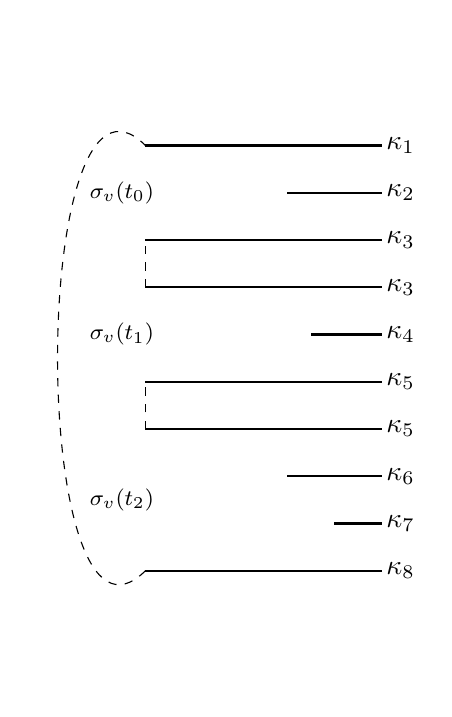
\begin{tikzpicture}[scale=0.6]
    \tikzset{->-/.style={decoration={ markings,
                mark=at position #1 with {\arrow{>}}},postaction={decorate}}}
    \draw [black, thick=1.5] (-5,-1) to (0,-1);
    \draw [black, thick=1.5] (-5,2) to (0,2);
    \draw [black, thick=1.5] (0,0) to (-1,0);
     \draw [black, thick=1.5] (0,1) to (-2,1);

    \draw [black, thick=1.5] (-5,3) to (0,3);
    \draw [black, thick=1.5] (-5,5) to (0,5);
    \draw [black, thick=1.5] (0,4) to (-1.5,4);
 
    \draw [black, thick=1.5] (-5,6) to (0,6);
    \draw [black, thick=1.5] (-5,8) to (0,8);
     \draw [black, thick=1.5] (0,7) to (-2,7);

    \draw[black,dashed] (-5,2) to (-5,3);
    \draw[black,dashed] (-5,5) to (-5,6);

  \draw [black, dashed] (-5, -1) to[in=135,out=225] (-5,8);
    \node at (-5.5,0.5) {\footnotesize{$\sigma_v(t_2)$}}  ;
    \node at (-5.5,4) {\footnotesize{$\sigma_v(t_1)$}}  ;
    \node at (-5.5,7) {\footnotesize{$\sigma_v(t_0)$}}  ;

        \node at (0.4,-1) {$\kappa_8$};
        \node at (0.4,2) {$\kappa_5$};
        \node at (0.4,0) {$\kappa_7$}; 
        \node at (0.4,1) {$\kappa_6$};

        \node at (0.4,3) {$\kappa_5$};
        \node at (0.4,5) {$\kappa_3$};
        \node at (0.4,4) {$\kappa_4$};
        \node at (0.4,6) {$\kappa_3$};
        \node at  (0.4,8) {$\kappa_1$};
        \node at  (0.4,7) {$\kappa_2$};
    \end{tikzpicture}
    \caption{A configuration with 3 partial flow trees attached to $\sigma_v$ at the points $\sigma_v(t_0)$ ,
    $\sigma_v(t_1)$, $\sigma_v(t_2)$. The numbers on the right determines the gradient equation at
    that end. The dashed part represents the loop $\sigma_v$}   \label{adamsmap}
\end{figure}

Attaching partial flow trees to $\sigma_{v}\colon[0,r_{v}]\to Q$ then means fixing points $0\le t_{0}\le t_{1}\dots\le t_{m}\le r_{v}$ and partial flow trees $\Gamma_{j}$, $j=1,\dots,m$ that start at $\sigma_{v}(t_{j})$. Our map $\phi$ takes
values in $\Omega CM_{-\ast}(Q)$ and will accordingly be defined by attaching flow
trees which have no output at the co-unit. Note that the set of positive punctures of minimum free partial flow trees for a fixed
decreasing boundary numbering constitutes a codimension two subset in $Q$ and that the corresponding
subset for any numbering lies in an arbitrarily small neighborhood of it. Choosing the Morse data generically means in particular that the base point $q$ does not lie on any minimum free partial flow tree. 




If $\sigma_{v}\colon [0,r_{v}]\to Q$ is a loop with flow trees attached at $0\le t_{0}\le t_{1}\dots\le t_{m}\le r_{v}$, we also introduce a numbering of the components of $[0,r_{v}]-\{t_{1},\dots,t_{m}\}$ induced by the flow trees attached as follows. The right most interval $(t_{m},r_{v}]$ is numbered by $\kappa_{0}$. The right boundary segment of the strip with slits attached at $\sigma_{v}(t_{m})$ is numbered by $\kappa_{0}$ as well, whereas the left boundary segment of its domain is numbered by $\kappa_{k_{m}}$. 
We number the boundary segment $(t_{m-1},t_{m})$ and the right boundary segment of the domain of the flow tree attached at $\sigma_{v}(t_{m-1})$ by $\kappa_{k_{m}}$ as well. 
The left boundary segment of the flow tree attached at $\sigma_{v}(t_{m-1})$ is then numbered by $\kappa_{k_{m-1}}$, 
which determines the numbering of the segment $(t_{m-2},t_{m-1})$ as well as the right boundary
segment in the flow tree at $\sigma_{v}(t_{m-2})$, etc. We view the end result of this process as
the domain for a loop with flow trees attached with numbering $\kappa$ that decreases, see Figure
\ref{adamsmap}. 

Note next that if $\sigma\colon I^{d}\to\Omega Q$ is a $d$-dimensional cube in general
position with respect to $\bar f$, the set of $\sigma_{v}$, $v\in I^{d}$ for which a single partial
flow tree can be attached is at most $(d-1)$-dimensional. Attaching more partial flow trees, the
dimension decreases further, by at least one for each flow tree. We say that the loops in $\sigma$
with flow trees attached which form $0$-dimensional family are the rigid loops with flow trees in
$\sigma$. If $\sigma$ is a cubical simplex in $\Omega Q$ and if $\mathbf{y}$ is a word of critical points then we let 
\[
\mathcal{T}(\sigma;\mathbf{y})
\]
denote the space of loops with flow trees in $\sigma$, where the critical points at punctures of the flow trees read in order give the word $\mathbf{y}$. The dimension of $\mathcal{T}(\sigma;\mathbf{y})$ is then
\[
\dim(\mathcal{T}(\sigma;\mathbf{y}))=|\mathbf{y}|+\dim(\sigma)+(\ell(\mathbf{y})-1),
\]
where $\ell$ is the word length.

Note that if the set of loops in $\sigma$ with flow trees is transversely cut out then by definition
of the system of perturbing Morse functions, the loops with flow trees corresponding to a different
decreasing numbering $\kappa'$ is canonically diffeomorphic to that corresponding $\kappa$. We
define the map $\phi$ by counting rigid loops with flow trees in cubical simplices $\sigma$:
\begin{equation}\label{eq:deflooptotree}
\phi(\sigma)=\sum_{\dim(\mathcal{T}(\sigma;\mathbf{y}))=0}|\mathcal{T}(\sigma;\mathbf{y})|\mathbf{y}.
\end{equation}

\begin{rem}
	The map $\phi$ is defined only for chains that are suitably transverse to the Morse flow trees defined by the system of shifting functions $\bar f$. Since the Morse functions do not have any index one critical points a partial flow tree has at most $\dim(M)$ punctures. There is a natural evaluation map on partial flow trees that takes a flow tree to the location of its positive puncture. The image of this map for partial flow trees not involving the minimum is a stratified space of codimension one and by definition of the perturbation scheme the corresponding set for partial flow trees defined by distinct boundary numberings lie arbitrarily close to each other. The map $\phi$ above is defined for chains of loops with evaluation maps that are smooth and transverse to this stratified subset. It is straightforward to see that any chain of loops is homotopic to such a transverse chain and that any two transverse chains that are homologous are homologous through a transverse chain of loops. This means that we can replace all chains by chains that represent these transversality conditions. 
\end{rem}

In order to connect this to the path loop fibration we consider a similar map
\[
    \hat{\phi} \colon C_{-\ast}(\mathrm{P} Q)\to \Omega CM_{-\ast}(Q)\otimes^{\t} CM_{-\ast}(Q),
\]
where $\t$ denotes the canonical twisting cochain of the cobar construction and $\mathrm{P}Q$ the based path
space. The map $\hat{\phi}$ again counts rigid paths with flow trees, where a path with flow trees is defined as a loop with flow trees except that we also attach a flow tree at the endpoint of the path. Furthermore, the last puncture in the flow tree attached at the endpoint is the distinguished last factor and is allowed to be the co-unit critical point. (Other punctures are still not the co-unit critical point, which means that flow trees before the last are still co-unit free and that in the last flow tree only the last puncture is allowed to be the co-unit). We point out that the differential on the twisted complex acting on the last factor in the right hand side counts trees where the last puncture is distinguished.

\begin{lem}
    The maps $\phi$ and $\hat{\phi}$ are chain maps.
\end{lem}

\begin{proof}
	To see this note that the contributions to the chain map equation in both cases correspond to the boundary of an oriented compact 1-dimensional manifold. 
\end{proof}

\begin{rem}
	The codimension one boundary of $\mathcal{T}(\sigma;\mathbf{y})$ corresponds either to the loop or path moving to the boundary of $\sigma$ or to the breaking of a flow tree at a critical point. 
	Instances when two trees are attached at the same point are naturally interior points of the
    moduli space where the disks with slits joins to a new disk with a slit of width equal to the
    sum of the widths. See Figure \ref{interiorpoints}.
\end{rem}

\begin{figure}[h!]
    \centering
    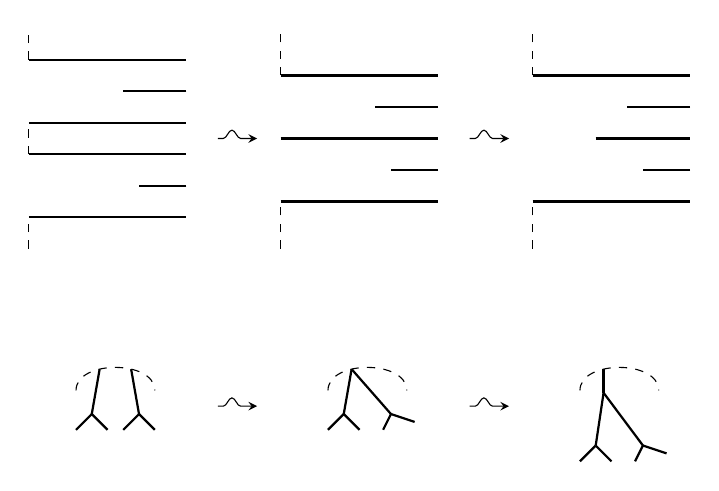
\begin{tikzpicture}[scale=1]
    \tikzset{->-/.style={decoration={ markings,
                mark=at position #1 with {\arrow{>}}},postaction={decorate}}}

        \begin{scope}[scale=0.4]
    \draw [black, thick=1.5] (-5,3) to (0,3);
    \draw [black, thick=1.5] (-5,5) to (0,5);
    \draw [black, thick=1.5] (0,4) to (-1.5,4);
 
    \draw [black, thick=1.5] (-5,6) to (0,6);
    \draw [black, thick=1.5] (-5,8) to (0,8);
     \draw [black, thick=1.5] (0,7) to (-2,7);

    
     \draw[black,dashed] (-5,2) to (-5,3);
    \draw[black,dashed] (-5,5) to (-5,6);
   \draw[black,dashed] (-5,8) to (-5,9);
   \end{scope} 

    \draw[-stealth,decorate,decoration={snake,amplitude=3pt,pre length=2pt,post length=3pt}]
    (0.4,2.2) -- ++(0.5,0);



        \begin{scope}[scale=0.4, xshift=8cm]
    \draw [black, thick=1.5] (-5,3.5) to (0,3.5);
    \draw [black, thick=1.5] (0,4.5) to (-1.5,4.5);
 
    \draw [black, thick=1.5] (-5,5.5) to (0,5.5);
    \draw [black, thick=1.5] (-5,7.5) to (0,7.5);
     \draw [black, thick=1.5] (0,6.5) to (-2,6.5);

    
     \draw[black,dashed] (-5,2) to (-5,3.5);
   \draw[black,dashed] (-5,7.5) to (-5,9);
   \end{scope} 

    \draw[-stealth,decorate,decoration={snake,amplitude=3pt,pre length=2pt,post length=3pt}]
    (3.6,2.2) -- ++(0.5,0);




        \begin{scope}[scale=0.4, xshift=16cm]
    \draw [black, thick=1.5] (-5,3.5) to (0,3.5);
    \draw [black, thick=1.5] (0,4.5) to (-1.5,4.5);
 
    \draw [black, thick=1.5] (-3,5.5) to (0,5.5);
    \draw [black, thick=1.5] (-5,7.5) to (0,7.5);
     \draw [black, thick=1.5] (0,6.5) to (-2,6.5);

    
     \draw[black,dashed] (-5,2) to (-5,3.5);
   \draw[black,dashed] (-5,7.5) to (-5,9);
   \end{scope} 

        \begin{scope} [yshift=-1cm, xshift=-1.4cm]  

   \draw[black, dashed] (0,0) to[in=90, out=90] (1,0);  
   
   \draw[black, thick=1] (0.3,0.27) to (0.2, -0.3); 
   \draw[black, thick=1] (0.2, -0.3) to (0, -0.5); 
   \draw[black, thick=1] (0.2, -0.3) to (0.4, -0.5); 

   \draw[black, thick=1] (0.7,0.27) to (0.8, -0.3); 
   \draw[black, thick=1] (0.8, -0.3) to (1, -0.5); 
   \draw[black, thick=1] (0.8, -0.3) to (0.6, -0.5); 

    \end{scope} 

 \draw[-stealth,decorate,decoration={snake,amplitude=3pt,pre length=2pt,post length=3pt}]
    (0.4,-1.2) -- ++(0.5,0);



 \begin{scope} [yshift=-1cm, xshift=1.8cm]  

   \draw[black, dashed] (0,0) to[in=90, out=90] (1,0);  
   
   \draw[black, thick=1] (0.3,0.27) to (0.2, -0.3); 
   \draw[black, thick=1] (0.2, -0.3) to (0, -0.5); 
   \draw[black, thick=1] (0.2, -0.3) to (0.4, -0.5); 

   \draw[black, thick=1] (0.3,0.27) to (0.8, -0.3); 
   \draw[black, thick=1] (0.8, -0.3) to (1.1, -0.4); 
   \draw[black, thick=1] (0.8, -0.3) to (0.7, -0.5); 

    \end{scope} 

 \draw[-stealth,decorate,decoration={snake,amplitude=3pt,pre length=2pt,post length=3pt}]
    (3.6,-1.2) -- ++(0.5,0);



 \begin{scope} [yshift=-1cm, xshift=5cm]  

   \draw[black, dashed] (0,0) to[in=90, out=90] (1,0);  
 
   \draw[black, thick=1] (0.3, 0.27) to (0.3, -0.03);
   \draw[black, thick=1] (0.3,-0.03) to (0.2, -0.7); 
   \draw[black, thick=1] (0.2, -0.7) to (0, -0.9); 
   \draw[black, thick=1] (0.2, -0.7) to (0.4, -0.9); 

   \draw[black, thick=1] (0.3,-0.03) to (0.8, -0.7); 
   \draw[black, thick=1] (0.8, -0.7) to (1.1, -0.8); 
   \draw[black, thick=1] (0.8, -0.7) to (0.7, -0.9); 




 \end{scope} 







    \end{tikzpicture}
    \caption{Flow trees attached at the same point are interior points: in the source (top),
in the target (bottom). }\label{interiorpoints} \end{figure}




With this established we can now prove Adams result:
\begin{thm}\label{thm:Adams}
	The flow tree map $\phi\colon C_{-\ast}(\Omega Q)\to \Omega CM_{-\ast}(Q)$ is a quasi-isomorphism.
\end{thm}

\begin{proof} The first observation is that the chain complex $\Omega CM_{-\ast}(Q)\otimes^{\t}
    CM_{-\ast}(Q)$ is acyclic. To see that, note that for each critical point $y$ there is a unique
    flow tree with positive puncture $y$ and two negative punctures, one at the co-unit $x$ and one at $y$.
    Filtering by degree we find that this is the only part of the differential which contributes to
    the differential on the first page of the corresponding spectral sequence. Since it gives an isomorphism from words not ending with the co-unit $x$ to those which does end with
    $x$, the desired acyclicity follows. Clearly, $C_{-\ast}(\mathrm{P}Q)$ is also acyclic. 
	
    Note next that the map $\hat{\phi}$ respects the filtration by degree at the end point. The corresponding $E_{1}$-terms with induced maps are
	\[
        C_{-\ast}(Q;H_{-\ast}(\Omega Q))  \to H_{\ast}(\Omega CM_{-\ast}(Q)\otimes CM_{-\ast}(Q)),	\] 
	and $E_{2}$-terms
	\[
	H_{-\ast}(Q;H_{-\ast}(\Omega Q))  \to H_{-\ast}(Q;H_{\ast}(\Omega CM_{-\ast}(Q))).
	\] 
    Zeeman's comparison theorem \cite[Sec. 3.3]{McCleary} then establishes the result.
\end{proof}

\begin{rem}\label{r:dim4}
	If $\dim(Q)=4$ then the Morse function may have critical points of index one. In this case we
    use stabilization as follows. Multiply $Q$ by $\R^{N}$ for any $N \geq 2$, and consider the function $F(q,x)=f(q)+x^{2}$, then $F$ has the same critical points as $f$ and $-\nabla F$ is inward point at infinity.  In $Q\times \R^{N}$ there is room to cancel 1-handles and the above applies. In this case we define $CM_{-\ast}(Q)$ to be $CM_{-\ast}(Q\times \R^{N})$  (which is a 1-reduced version of the original complex). Noting that $C_{-\ast}(Q\times \R^{N})$ and $C_{-\ast}(Q)$ are canonically isomorphic the result follows also in this case.   
\end{rem}


We next show that $CE^{\ast}_{\parallel}(\Lambda)$ and $CE^{\ast}(\Lambda)$ are isomorphic if $\Lambda$ is simply connected.
This is a more or less direct consequence of the description of rigid disks on a Legendrian with parallel copies and the isomorphism in Theorem \ref{thm:Adams}. Since components in $\Lambda_{-}$ are not affected by this choice of $CE^{\ast}_{\parallel}$ versus $CE^{\ast}$, we disregard them and assume that $\Lambda=\Lambda_{+}$ in what follows.

Recall the definition of $CE^{\ast}(\Lambda)$ given in Remark \ref{r:topologicalversion}, generated by
chains $C_{-\ast}((\Omega_{p}\Lambda)^{\times (i+1)})$ in the product of the based loop space of $\Lambda$ with factors separated by Reeb chords. Here the differential of a chain in the product $C_{-\ast}(\Omega\Lambda)^{\times (i+1)}$ of the based loop space of $\Lambda$ with factors separated by Reeb chords. Here the differential of a chain
is just the usual differential of the chain whereas the differential of a Reeb chord is a sum over
all moduli spaces of disks with one positive puncture at the chord and any number of negative
punctures. Such a moduli space carries a fundamental chain and the contribution to the differential is alternating word of chains in the based loop space corresponding to the boundary arcs of the disk carried by the fundamental chain and Reeb chords at the negative puncture:
\[
d c_{0} = \sum_{\mathbf{c}'}[\mathcal{M}^{\sy}(\mathbf{c})],
\]  
where $\mathbf{c}=c_{0}\mathbf{c}'$ and $\mathbf{c}'$ is a word of Reeb chords.

We next consider a system of parallel copies $\bar\Lambda=\{\Lambda_{j}\}_{j=0}^{\infty}$ defined by a system of positive Morse functions $\bar f=\{f_{j}\}_{j=1}^{\infty}$, where $\Lambda_{0}=\Lambda$. Recall that the generators of the algebra $CE^{\ast}_{\parallel}(\Lambda)$ are the Reeb chords connecting $\Lambda_{0}$ to $\Lambda_{1}$, and that these are long, corresponding to Reeb chords of $\Lambda$ and short, corresponding to critical points of $f_{1}$, except for the minimum. The differential counts rigid disks with one positive puncture in $\mathcal{M}^{\sy}(\mathbf{b};\kappa)$ where $\kappa$ is a decreasing boundary numbering, $\mathbf{b}=b_{0}\mathbf{b}'$. 

If $\mathbf{b}'$ is a word of Reeb chords let $\mathbf{b}'_{\mathrm{lo}}$ denote the word obtained by removing all short Reeb chords and $\mathbf{b}'_{\mathrm{sh}}$ that obtained by removing all long Reeb chords. Let $\bar{\Lambda}_{\delta}$ denote the system of parallel copies defined by the system $\delta\bar f$.

\begin{thm}\label{t:quantumflowtree}
	For all sufficiently small $\delta>0$ there is a natural one to one correspondence between rigid holomorphic disks with one positive puncture in $\mathcal{M}^{\sy}(\mathbf{b};\kappa)$ and rigid configurations of a holomorphic disk with boundary on $\Lambda$ in $\mathcal{M}^{\sy}(b_{0}\mathbf{b}'_{\mathrm{lo}})$ with partial flow trees attached along the boundary, where the partial flow trees have negative punctures corresponding to $\mathbf{b}'_{\mathrm{sh}}$ and such that the total word of negative asymptotics is $\mathbf{b}'$. 
\end{thm} 

\begin{proof}
	This was proved in the setting of knot contact homology in \cite[Corollary 5.14, 5.19, and 5.20]{E} and in the case when there is only one flow line attached in \cite[Theorem 3.6]{EESa}. The proof has three parts, convergence, gluing, and surjectivity of gluing. All relevant technicalities in this more general case can be handled as there. 
\end{proof}

We next consider the map 
\[
\phi\colon CE^{\ast}(\Lambda)\to CE^{\ast}_{\parallel}(\Lambda),
\]
which takes every Reeb chord to itself and takes a chain $\sigma$ in the based loop space to $\phi(\sigma)$, where $\phi$ is as in \eqref{eq:deflooptotree} and where we identify the critical points of $f_{1}$ with the corresponding Reeb chords connecting $\Lambda_{0}$ to $\Lambda_{1}$.

\begin{thm}\label{t:parallel=loops}
	The map $\phi$ is a DG-algebra map and	
	if $\Lambda^{+}$ is simply connected then $\phi$ is a quasi-isomorphism. 		
\end{thm}

\begin{proof}
	The fact that $\phi$ is a chain map follows from Theorem \ref{t:quantumflowtree}.
	Filter the algebras by action of Reeb chords in the left hand side and actions of long Reeb chords in the right hand side. The map respects this filtration and gives an isomorphism on the $E_{2}$-pages by Theorem \ref{thm:Adams}. Since the sum actions of the Reeb chords at the negative end is bounded by that at the positive the spectral sequences converges. The theorem follows.  
\end{proof}

\begin{rem}\label{r:dim4iso}
	Note that the isomorphism in Theorem \ref{t:parallel=loops} is compatible with the stabilization of Remark \ref{r:dim4}. To see this we multiply the ambient contact manifold $Y$ with contact form $\alpha$ by $T^{\ast}\R^{N}$ and consider $\Lambda\times\R^{N}\subset Y\times T^{\ast}\R^{N}$ with contact form $\theta=(\alpha - y\cdot dx)$. The Reeb chord of $\Lambda\times\R^{N}$ then come in $\R^{N}$-families, one for each Reeb chord of $\Lambda$. Consider the contact form $e^{x^{2}}\theta$ and note that with respect to this contact form the Reeb chords of $\Lambda\times\R^{N}$ are in natural one to one correspondence with those of $\Lambda$ and there is a canonical isomorphism between $CE^{\ast}(\Lambda)$ and $CE^{\ast}(\Lambda\times\R^{N})$. In fact the disks in the differential are canonically identified. It follows in particular, that Theorem \ref{t:parallel=loops} holds also if $\dim(Q)\le 4$.   
\end{rem}

\section{Lagrangian (co)algebra}
As before, $X$ is a Liouville manifold with $c_1(X)=0$ and $L$ is an
exact relatively spin Lagrangian in $X$ with vanishing Maslov class and ideal boundary given by the Legendrian $\Lambda$. 

We will associate several chain level structures to $L$. To begin with, let us first assume that $L$
is an embedded Lagrangian. Since $L$ has boundary, in classical topology, one can consider either $C^*(L)$ or $C^*(L,
\partial L)$. In our case, these two choices are reflected in the choices of $+$ or $-$ decorations
on $L$, respectively. More generally, let $L^{v}$, $v\in \Gamma$ be the (irreducible) components of $L$. As
with the Legendrian submanifolds in Section \ref{ssec:Leginv}, we assume these components of
$L$ are decorated by signs and we write $L=L^{+}\cup L^{-}$ for the corresponding decomposition. 
Let $F\colon L\to\R$ be a Morse function with prescribed behaviour at infinity (depending on
the $+$ or $-$ decoration) as explained in
Section \ref{sec:parallel}. We use this to construct a system of parallel copies $\bar
L=\{L_{j}\}_{j=1}^{\infty}$, as in Section \ref{sec:parallel}, shifted at
infinity along the Reeb flow either in the positive or negative direction on $L^{+}$ and $L^{-}$, respectively. 

Now, using the parallel copies, $\{L_j\}_{j=1}^\infty$, we define a graded quiver $\mathcal{Q}_L$ as
follows. The parallel copies $\{L_j \}_{j=1}^\infty$ give rise to following sets, fix $i_1< i_2$
positive integers, and $v,w \in \Gamma$ with $v \neq w$: \begin{itemize} 
    \item Intersection points $L^v_{i_1} \cap L^v_{i_2}$ in bijection with the union of critical points of
        $F|_{L_v}$. (These critical points may depend on the $+$ or $-$ decoration on $L_v$, for example, one can turn a $-$ decorated component $L^v$ into $+$ decorated, by introducing critical points corresponding to the topology of $\partial L_v$, see Figure
\ref{intersectiongen}).   
    \item Intersection points $L^v_{i_1} \cap L^w_{i_2}$ in bijection with $L^v \cap L^w$.  
    \end{itemize}

\begin{figure}[h!]
    \centering
    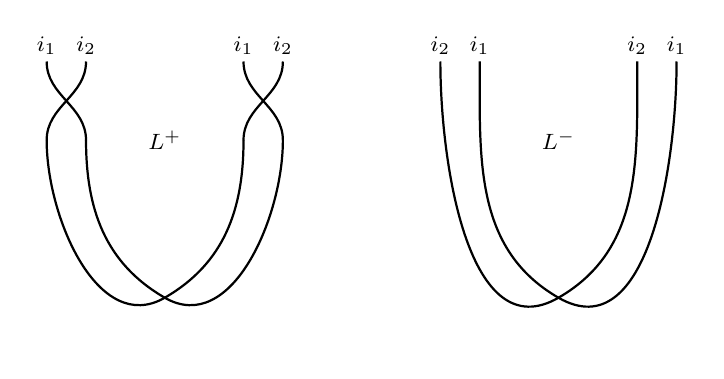
\begin{tikzpicture}[scale=1]
    \tikzset{->-/.style={decoration={ markings,
                mark=at position #1 with {\arrow{>}}},postaction={decorate}}}
    \draw [black, thick=1.5] (1.5,3) to[in=330,out=270] (0,0);
    \draw [black, thick=1.5] (0,0) to[in=270,out=150] (-1,3);
    \draw [black, thick=1.5] (0,0) to[in=270,out=210] (-1.5,3);
    \draw [black, thick=1.5] (0,0) to[in=270,out=30] (1,3);
   
    \draw [black, thick=1.5] (-3.5,2) to[in=330,out=270] (-5,0);
    \draw [black, thick=1.5] (-3.5,3) to[in=90,out=270] (-4,2);
    \draw [black, thick=1.5] (-4,3) to[in=90,out=270] (-3.5,2);
     \draw [black, thick=1.5] (-5,0) to[in=270,out=30] (-4,2);
   
    \draw [black, thick=1.5] (-6.5,3) to[in=90,out=270] (-6,2);
    \draw [black, thick=1.5] (-6,3) to[in=90,out=270] (-6.5,2);
    \draw [black, thick=1.5] (-5,0) to[in=270,out=150] (-6,2);
    \draw [black, thick=1.5] (-5,0) to[in=270,out=210] (-6.5,2);

    \node at (1.5,3.2) {\footnotesize{$i_1$}}  ;
    \node at (1,3.2) {\footnotesize{$i_2$}}  ;
    \node at (-1.5,3.2) {\footnotesize{$i_2$}}  ;
     \node at (-1,3.2) {\footnotesize{$i_1$}}  ;

    \node at (-3.5,3.2) {\footnotesize{$i_2$}}  ;
    \node at (-4,3.2) {\footnotesize{$i_1$}}  ;
    \node at (-6.5,3.2) {\footnotesize{$i_1$}}  ;
     \node at (-6,3.2) {\footnotesize{$i_2$}}  ;

    \node at (0, 2) {\footnotesize{$L^{-}$}}; 
    \node at (-5, 2) {\footnotesize{$L^{+}$}}; 


    \end{tikzpicture}
    \caption{Difference between $+$ and $-$ generators. Both the left and the right hand side depicts shifts corresponding to Morse functions with a maximum. One of the intersection points in $L_{+}$ is the minimum and corresponds to the unit for the Floer cohomology product.}
    \label{intersectiongen}
\end{figure}

Furthermore, by the construction in Section \ref{sec:parallel}, there are canonical bijections between the above sets associated
to any pairs $(i_1, i_2)$ and $(i'_1, i'_2)$ with $i_1 < i_2$ and $i'_1 < i'_2$. So, fix a pair $(i_1,i_2)$ such that $i_1 < i_2$
and define a graded quiver $\mathcal{Q}_L$ with vertex set $\Gamma$ and with an arrow connecting $v$
to $w$ (possibly equal to $v$) for each element of the above sets. Let $\mathcal{I}$ denote
the set of arrows. 

Alternatively, one can describe the generators as the set of intersection points in $L_{0}\cap L_{1}$, between the original $L$ and the first shifted copy.

Let $CF^*(L)$ be the graded $\k$-bimodule generated by $\mathcal{I}$. Thus, there is one generator $x_{vw}$ in degree $|x_{vw}|$ for each arrow in $\mathcal{Q}_L$ from $v$ to $w$.  We endow $CF^{\ast}(L)$ with the structure of an $A_{\infty}$-algebra. Let $x_{0}$ be an intersection point generator and let $\mathbf{x}'=x_{i}\dots x_{1}$ be a word of intersection points. Consider the disk $D_{i+1}$ with $i+1$ boundary punctures and with a decreasing numbering of its boundary arcs $\kappa$. Let $\mathbf{x}=x_{0}x_{i}\dots x_{1}$.  Consider the moduli space $\mathcal{M}^{\fl}(\mathbf{x};\kappa)$.  Define the operations $\m_{i}$ by
\[ 
\m_{i}(\mathbf{x}') = \sum_{\ell(\mathbf{x}')=i, |x_{0}|=|\mathbf{x}'|+(2-i)} |\mathcal{M}^{\fl}(\mathbf{x};\kappa)|x_{0}
\] 
where $\ell(\mathbf{y})$ denotes the word length of $\mathbf{y}$ and where $|\mathcal{M}^{\fl}(\mathbf{x};\kappa)|$ denotes the algebraic number of points in the oriented 0-dimensional manifold.

\begin{lem}
The operations $\m_{i}$ satisfy the $A_{\infty}$-algebra relations. 
\end{lem}

\begin{proof}
This follows by the usual argument: after noting that the decreasing boundary numbering ensures that there is no boundary bubbling, one observes that the terms in the $A_{\infty}$-algebra relations count the ends of a 1-dimensional oriented compact manifold by Theorems \ref{thm:mdlitv} and \ref{thm:mdlicmpct}. Note also that the operations compose because of Theorem \ref{thm:mdlicopies}.
\end{proof}

We call $CF^{\ast}(L)$ the Lagrangian Floer cohomology algebra of $L$. Note that there is an
idempotent $e_{v}$ on each component $L_{v}\subset L^{+}$ corresponding to the  minimum of the
shifting Morse function, which is increasing at infinity since we shift in the positive Reeb
direction. We write $\k_{+}$ for the sum of $\mathbb{K}e_{v}$ over all components in $L^{+}$. We
write $\k_{-} \oplus CF^*(L)$ for the augmented algebra where we adjoined an idempotent $e_{w}$
for each component $L_w\subset L^{-}$. (On these components the shifting function is decreasing at
infinity and has a maximum rather than a minimum in the compact part.) Note that this is a connected
algebra over $\k$. 

\begin{rem} The two different choices of perturbations at infinity corresponding to $+$ and $-$ are
    the two extremal constructions where one pushes the copies either always in positive direction or
    always in the negative direction. One can also choose perturbations at infinity to depend on the
    topology of the manifold at infinity (see, for example, Section 4 of
    \cite{abouzaid}). All our constructions should extend meaningfully to this more
    general setting but we have not pursued this direction in this paper.
\end{rem} 



We next consider various linear duals of $CF^{\ast}(L)$ and associated algebraic objects. The
simplest case occurs when $CF^{\ast}(L)$ is simply connected. In this case the linear dual
$CF_{\ast}(L)$ is a coalgebra with operations $\Delta_{i}$ dual to $\m_{i}$, and as before we can
adjoin $\k_-$ so that $\k_- \oplus CF_*(L)$ is co-augmented over $\k$. Then, we define the  
\emph{Adams-Floer DG-algebra}
\[ 
\Omega (\k_{-} \oplus CF_*(L)),
\]
by applying the cobar construction.

In the non-simply connected case, we replace this object by the \emph{completed Adams-Floer DG-algebra}: 
\[
(\Bar (\k_{-} \oplus CF^*(L)))^\#.
\]


% and is simply-connected over $\k$ if each component of $L$ is simply-connected. 
%
%Note that this coalgebra does not have a counit. We write $\k \oplus CF_*(L,L)$ for the coaugmented
%coalgebra where we adjoined a counit. Note that this is a connected coalgebra over $\k$ (though,
%topologically $L$ may be disconnected), and is simply-connected over $\k$ if each component of $L$
%is simply-connected. We call $CF_{\ast}(L,L)$ the Lagrangian Floer homology coalgebra of $L$. 

%Let $CF^*(L,L)$ denote the dual of the module $CF_{\ast}(L,L)$ we endow $CF^*(L,L)$ with the structure of an $A_\infty$-algebra with operations $m_i$ corresponding exactly to the $\Delta_{i}$, switching the roles of input and output. It follows from Lemma \ref{label} that the operations $m_{i}$ compose and satisfy the $A_{\infty}$-relations.
%again the moduli space $\mathcal{M}^{\co}=\mathcal{M}^{\co;\kappa}$ is defined by decorating the boundary of the source disk with labeling that is increasing at all punctures except the negative puncture. Lemma \ref{label} shows that the moduli spaces corresponding to different labelings are canonically isomorphic and that the operations are thus well defined and satisfy the $A_{\infty}$-algebra relations. 

\begin{ex} Let $L$ be the standard Lagrangian $D^n$ filling the standard Legendrian unknot $\Lambda
    \subset S^{2n-1}$. The Floer cohomology can be computed as follows:
\[ 
CF^*(L) =
\begin{cases}
\mathbb{K}x,\, |x|=0, &\text{if $L$ is decorated with $+$,}\\
\mathbb{K}c,\, |c|=n.   & \text{if $L$ is decorated with $-$.}
\end{cases}
\]
Alternatively, if we want compatibility with the inclusion $C^{\ast}(D^{n},\partial D^{n})\to C^{\ast}(D^{n})$ as
\[ 
CF^*(L) =
\begin{cases}
\mathbb{K}c \oplus \mathbb{K} y \oplus \mathbb{K} x,\\ 
|c|=n, |y|=n-1, |x|=0,\,
dy =c &\text{if $L$ is decorated with $+$,}\\
\mathbb{K}c,\, |c|=n.   & \text{if $L$ is decorated with $-$.}
\end{cases}
\]
\end{ex}

In Section \ref{sec:CWnoHam}, we introduce a model for wrapped Floer cohomology without Hamiltonian term and
prove it is quasi-isomorphic to the usual wrapped Floer cohomology. We refer to there for details
and give only a short description here. The chain complex underlying $CW^{\ast}(L)$ is the
following. Let $L=L_0$ and shift $L$ off itself to $L_{1}$ by a Morse function that is positive at
infinity (as in the definition of parallel copies when $L$ is decorated $+$). The generators of $CW^{\ast}(L)$ are then Reeb chords connecting $L_{1}$ to $L_{0}$ and intersection points in $L_{0}\cap L_{1}$.

There is an $A_\infty$ functor, often called the \emph{acceleration functor}, 
\[ CF^*(L) \to CW^*(L). \]
If $L$ is decorated $+$, it can be shown that this functor is unital. 


%
%Consider now $CF^{\ast}(L)$. Here $L^{+}$ is shifted like in the definition of $CW^{\ast}(L)$ at
%infinity, whereas $L^{-}$ is not. To build a shifting function for $L^{-}$, we add a cylindrical
%Lagrangian $\widehat{L}^{-} \approx [0,\infty)\times \Lambda^{-}$ to the boundary $\Lambda^{-}$ of
%$L^{-}$ which intersects the trivial cylinder $[0,\infty)\times \Lambda^{-}$ cleanly along
%$\{T\}\times \Lambda^{-}$ so that it is shifted away from $\Lambda^{-}$ in the positive Reeb
%direction at infinity. After small perturbation we then get intersection point between
%$\widehat{L}^{-}$ and $[0,\infty)\times\Lambda^{-}$ corresponding to the Morse complex of
%$\Lambda^{-}$. It then follows from our definition of $CW^{\ast}(L)$ that $CF^{\ast}(L)$ is a
%subalgebra, where the corresponding quotient complex is generated by Reeb chords of $L$ at infinity
%and by the Morse complex of $\Lambda^{-}$. 



%Statement of the Theorem that says that $CW^*(L,L)$ is quasi-isomorphic to $LCA^*(\Lambda)$ as an
%$A_\infty$ algebra. (Proof is in the appendix). 



\section{Maps relating Legendrian and Lagrangian (co)algebras}\label{Sec:LegLag}
We continue with our usual set-up, where $X$ is Liouville manifold with $c_1(X)=0$ and $L$ is an
exact Lagrangian in $X$ with vanishing Maslov class and ideal boundary given by the Legendrian
$\Lambda$. Let $\Gamma$ be the set of embedded components of $L$ subdivided into
$\Gamma^{+}\cup\Gamma^{-}$. Let $\Theta$ be the set of components of $\Lambda$ with induced
subdivision $\Theta^{+}\cup\Theta^{-}$. 

In this section we will define twisting cochains relating the parallel copies version $CE^{\ast}_{\parallel}(\Lambda)$ and the Floer cohomology $CF^{\ast}(L)$. Since $L$ is an exact filling, we have an augmentation $\epsilon_L \colon CE^{\ast}(\Lambda) \to \k$. As in Section \ref{ssec:Leginv} we use this augmentation throughout to change coordinates in such a way
that $\Delta_{0}=0$. As usual let $LC_{\ast}^{\parallel}(\Lambda)$ denote the corresponding co-unital coalgebra with co-unit 
\[ 
\sum_{v\in\Theta^{+}} x_{v} + \sum_{w\in\Theta^{-}} e_{v},
\]
and let $\eta\colon \k\to LC_{\ast}^{\parallel}(\Lambda)$ denote the co-augmentation
\[ 
\eta(e_{v})=
\begin{cases}
x_{v} &\text{if $v\in\Theta^{+}$},\\
e_{v} &\text{if $v\in\Theta^{-}$},
\end{cases}
\]
see \eqref{eq:coaugparallel},
so that $CE^{\ast}_{\parallel} = \Omega LC_{\ast}^{\parallel} $. Note that this
means that $x_v$ are traded for $e_v$ for $v \in \Theta^+$. Specifically, write
$\overline{LC}_{\ast}^{\parallel}$ for $\mathrm{coker}(\eta)$ and $\k\oplus
\overline{LC}_{\ast}^{\parallel}$ for the corresponding strictly counital co-algebra. Then
we have \[ 
CE^{\ast}_{\parallel} = \Omega LC_{\ast}^{\parallel} := \Omega(\k\oplus\overline{LC}_{\ast}^{\parallel}(\Lambda))
\]
Consider the Floer cohomology $A_{\infty}$-algebra $CF^{\ast}(L)$. Recall that there exists a strict
idempotent $u_{v}\in CF^{\ast}(L)$ for each $v\in\Gamma^{+}$ corresponding to the minimum of the
shifting Morse function and that we make $CF^{\ast}(L)$ unital by adding an idempotent $e_{w}$ for each $w\in\Gamma^{-}$. We write the strictly unital algebra $\k_{-}\oplus CF^{\ast}(L)$. Let $\epsilon\colon \k_{-}\oplus CF^{\ast}(L)\to \k$ be the augmentation that maps $u_{v}$ to $e_{v}$ for $v\in\Gamma^{+}$ and $e_{w}$ to $e_{w}$ for $w\in\Gamma^{-}$. Consider the dual of the bar construction:
\[ 
\A=(B(\k_{-}\oplus CF^{\ast}(L)))^{\#},
\]
or in other words the completed Adams-Floer DG-algebra. In what follows it will be useful to represent $\A$ as a quotient. Consider adding extra idempotents $e_{v}$, $v\in\Gamma^{+}$ to $\k_{-}\oplus CF^{\ast}(L)$. This gives $\k\oplus CF^{\ast}(L)$ and we equip it with the trivial augmentation $\epsilon'$ which is the projection to $\k$. Let
\[ 
\A'=(B(\k\oplus CF^{\ast}(L)))^{\#},
\] 
and let $\mathscr{I}$ denote the subalgebra of $\A'$ generated by all monomials that contains a dual of $u_{v}$ for some $v\in\Gamma^{+}$. Let $\rho\colon \A'\to\A$ denote the restriction map.

\begin{lem}
The map $\rho$ is a chain map with kernel $\mathscr{I}$. Consequently, $\A$ is quasi-isomorphic to $\A'/\mathscr{I}$. 
\end{lem}

\begin{proof}
It is clear that $\mathscr{I}$ is the kernel of $\rho$. The fact that $\rho$ is a chain map follows from the $u_{v}$ being strict idempotents.
\end{proof}

%and $\A := \Omega (\k
%\oplus CF_*(L,L))$ be the Adams-Floer DG-algebra of $L$. 
%and $\widehat{\A} := (\Bar
%(\k \oplus CF^*(L,L)))^\#$  its completion.
%Note that we have a natural map $\A \to \widehat{\A}$. We say that $\A$ is complete if this natural
%map is a quasi-isomorphism. For example, $\A$ is complete if $L$ is simply-connected.

We next define a map
\[ 
\t'\colon LC_*^{\parallel}(\Lambda) \to \A', 
\]
which will induce a twisting co-chain
\[ 
\t\colon \k\oplus \overline{LC}_{\ast}^{\parallel}(\Lambda)\to\A.
\]
The map $\t'$ is defined by the following curve count for generators of $LC_{\ast}^{\parallel}(\Lambda)$.
Fix systems of parallel copies $\bar L$ of $L$. Let $c$ be a Reeb chord of $\bar{\Lambda}$ and let $\mathbf{x}_{0}=x_{0;1}\dots x_{0;j}$ be a word of intersection points of $L$. Let 
\[ 
\mathbf{c}=c\mathbf{x}_{0}
\]
and define
\begin{equation}\label{eq:deft'}
\t'(c)=\sum_{|\mathbf{x}_{0}|=|c|+(1-i)}
|\mathcal{M}^{\fl}(\mathbf{c})|\mathbf{x}_{0}.
\end{equation}
We then have the following.

\begin{prop}\label{twch}
If $v\in\Theta^{+}$ is such that $\Lambda_{v}$ is a boundary component of $L_{w}$ for $w\in\Gamma^{+}$ then
\[ 
\t'(x_{v})= u_{w}',
\] 
where $u_{w}'$ is the dual of the idempotent $u_{w}$. Furthermore,
$\t'$ satisfies the equation of a twisting cochain. 
\end{prop} 

\begin{proof} 
For the first property we need to understand rigid holomorphic disks with positive puncture at the
    Reeb chord $x_{v}$. By small action such a holomorphic disk must lie in a neighborhood of
    $L_{w}$ and is hence given by Morse flow trees. There is only one flow line emanating from the
    minimum in $\Lambda_{v}$ and the flow line generically ends at the minimum of the shifting of
    $L_{w}$, see Figure \ref{mintomin}. The first equation follows. 	
	
To see the twisting co-chain equation,	
we need to check that 
\[ 
\m_1 \circ \mathfrak{t}' - \mathfrak{t}' \circ \Delta_1 + \sum_{d \geq 2} (-1)^d \m_2^{(d)}
\circ {\mathfrak{t}'}^{\otimes_\k d} \circ \Delta_d = 0 
\]
where $\m_2^{(2)} := \m_2$, and $\m_2^{(i)} := \m_2\circ (\mathrm{Id}_\A \otimes_\k \m_2^{(d-1)})$. 
To this end, we consider the boundary of the $1$-dimensional moduli space $\mathcal{M}^{\co}(c_{0}\mathbf{x})$. By Theorem \ref{thm:mdlicmpct} this corresponds to two level curves which by Theorems \ref{thm:mdlitv} and \ref{thm:mdlicopies} form the boundary of an oriented compact 1-manifold. 
\end{proof}

\begin{figure}[h!]
    \centering
    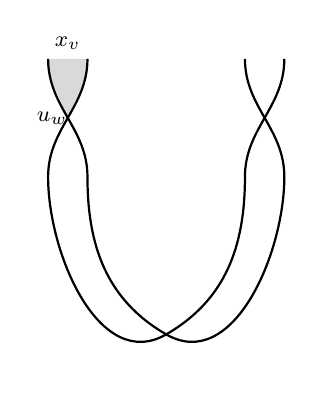
\begin{tikzpicture}[scale=1]
    \tikzset{->-/.style={decoration={ markings,
                mark=at position #1 with {\arrow{>}}},postaction={decorate}}}
  

 \begin{scope} 
     \clip (-6.25,2.75) to[in=270,out=110] (-6.5, 3.5) to (-6, 3.5) to[in=70,out=270] (-6.25,2.75);

\clip[preaction={draw,fill=gray!30}] (-7,4) rectangle (-3,2);
                             \end{scope}
 

    \draw [black, thick=1.5] (-3.5,2) to[in=330,out=270] (-5,0);
    \draw [black, thick=1.5] (-3.5,3.5) to[in=90,out=270] (-4,2);
    \draw [black, thick=1.5] (-4,3.5) to[in=90,out=270] (-3.5,2);
     \draw [black, thick=1.5] (-5,0) to[in=270,out=30] (-4,2);
   
    \draw [black, thick=1.5] (-6.5,3.5) to[in=90,out=270] (-6,2);
    \draw [black, thick=1.5] (-6,3.5) to[in=90,out=270] (-6.5,2);
    \draw [black, thick=1.5] (-5,0) to[in=270,out=150] (-6,2);
    \draw [black, thick=1.5] (-5,0) to[in=270,out=210] (-6.5,2);

    \node at (-6.25,3.7) {\footnotesize{$x_v$}}  ;
     \node at (-6.45,2.75) {\footnotesize{$u_w$}}  ;



    \end{tikzpicture}
    \caption{Minimum $x_v$ is sent to the minimum $u_w$} 
    \label{mintomin}
\end{figure}


Proposition \ref{twch} shows that $\t'$ maps the ideal generated by $x_{v}$, $v\in\Theta^{+}$ into $\mathscr{I}\subset\A'$. Hence $\t'$ induces a map
\[ 
\t\colon \k\oplus \overline{LC}_{\ast}^{\parallel}(\Lambda)\to \A/\mathscr{I}=\A.
\]
Note that if $\eta'\colon \k\oplus \overline{LC}_{\ast}^{\parallel}(\Lambda)$ and $\epsilon\colon\A\to\k$ is the trivial augmentation then $\epsilon\circ\t=\t\circ\eta=0$.
\begin{cor}
The map $\t$ is a twisting co-chain.
\end{cor}

\begin{proof}
Since $\t'$ satisfies the twisting co-chain equation so does $\t$. 	
\end{proof}

This twisting cochain is always defined, and determines a map:
\begin{equation} \label{ingen} 
CE^*_{\parallel}(\Lambda) \to \A. 
\end{equation}
We next consider the question whether $\t \in \mathrm{Kos}(\C, \A)$.
The following theorem gives a sufficient condition for $\t$ to be Koszul: 

\begin{thm} \label{mainthm} Suppose that $LC_*(\Lambda)$ is locally finite, simply-connected $\k$-bimodule.
    Suppose, in addition, that $HW^*(L)=0$, then $\A$ is quasi-isomorphic to $\Omega(\k_{-}
    \oplus CF_*(L))$ and $\t \colon \C \to \A$ is a
    Koszul twisted cochain. In
    other words, the induced DG-algebra map:
    \[ CE^*(\Lambda) \to \A\approx \Omega (\k_{-} \oplus CF_*(L)) \]
is a quasi-isomorphism.
\end{thm}

\begin{cor}\label{cor:CE=loopspace} 
	In the situation of Theorem \ref{mainthm}, suppose that $L$ is connected and decorated by $-$ and that
    $\partial L = \Lambda$ is diffeomorphic to a sphere $S^{n-1}$. Writing $\overline{L} = L \cup_{\partial} D^n$, there exists a quasi-isomorphism of DG-algebras
    \[ CE^*(\Lambda) \to C_{-*}(\Omega \overline{L}), \] 
where $\Omega \overline{L}$ is the based loop space of $\overline{L}$. 
\end{cor} 
\begin{proof} We first note that there exists a quasi-isomorphism $\k \oplus CF^*(L) \to
    C^*(\overline{L})$ since $L$ is an exact Lagrangian. We next use Theorem \ref{mainthm}
    and Adams' cobar equivalence (\cite{adams}): \[ \Omega (C_*(\overline{L})) \simeq C_{-*}(\Omega
    {\overline{L}}) \]
    which holds for the simply-connected topological space $\overline{L}$.     
\end{proof}

Theorem \ref{mainthm} is obtained as a  corollary of Theorem \ref{doubledual} and the following
result:

\begin{thm} \label{ainfiso} Suppose that $HW^*(L) =0$. Then, there exists a quasi-isomorphism of augmented $A_\infty$-algebras:
    \[\Psi\colon \k_{-} \oplus CF^*(L) \to LA_{\parallel}^*(\Lambda), \] 
such that 
\[ 
\Psi(e_{v})=
\begin{cases}
\sum_{\Lambda_{w}\subset\partial L_{v}}e_{w} &\text{for $v\in\Gamma^{-}$},\\
\sum_{\Lambda_{w}\subset\partial L_{v}}x_{w} &\text{for $v\in\Gamma^{+}$}.
\end{cases}
\]
   
\end{thm}

Note that $HW^*(L)=0$ if $X$ is subcritical, or more generally a flexible Weinstein
manifold. 

\begin{proof} 
We construct an $A_\infty$ functor $\e = (\e_i)_{i \geq 1}$ where 
\[ 
\e_i \colon (CF^*(L))^{\otimes_{\k} i} \to LA_{\parallel}^*(\Lambda) 
\]
$\e_i$ are constructed by dualizing the components of the map $\t'$. More explicitly,
given $c_{0}$ and $\mathbf{x}_{0}=x_{0;n},\ldots, x_{0;1}$, write $\mathbf{c}=c_{0}\mathbf{x}_{0}$ as in \eqref{eq:deft'}, and define
\[ 
\e_i(\mathbf{x}_{0}) = 
\sum_{c_{0}\in\mathcal{R}} |\mathcal{M}^{\fl}(\mathbf{c})| c_{0} 
\]
The proof that $(\e_i)_{i \geq i}$ is an $A_\infty$ functor follows as in the proof of Proposition \ref{twch}. 

Now, we need to check that $\e_1$ is a quasi-isomorphism. In the case that $L=L^{-}$, this is a consequence of the exact sequence for wrapped Floer cohomology induced by the subdivision of the complex into high and low energy generators:
\[ 
\begin{CD}
0 @>>> CW^{\ast}_{0}(L) @>>> CW^{\ast}(L) @>>> CW^{\ast}_{+}(L) @>>> 0,
\end{CD}
\]
as follows. In terms of the version of wrapped Floer cohomology presented in Section
    \ref{sec:wrappediso}, the low energy sub-complex $CW^{\ast}_{0}(L)$ is generated by Lagrangian
    intersection points in $L_{0}\cap L_{1}$, where $L=L_{0}$ and $L_{1}$ is the first parallel copy
    of $L$, shifted by a positive Morse function $f$ that increases in the end, see Section
    \ref{sec:parallel}. The differential on $CW^{\ast}_{0}(L)$ counts holomorphic strips which is
    incoming along $L_{1}$ and outgoing along $L_{0}$ at the output puncture. Similarly, the high
    energy quotient $CW^{\ast}_{+}(L)$ is generated by Reeb chords connecting $\Lambda_{1}$ to
    $\Lambda_{0}$, the differential counts holomorphic strips interpolating between such Reeb
    chords.  Since $CW^{\ast}(L)$ is acyclic it follows that the connecting homomorphism $HW^{\ast}_{+}(L)\to HW^{\ast+1}_{0}(L)$   is an isomorphism. In order to connect this to $CF^{\ast}(L)$ and $LA_{\parallel}^{\ast}(\Lambda)$, renumber the parallel copies so that $L_{1}$ now lies in the negative Reeb direction of $L_{0}$ at infinity and the shifting function $f$ is replaced by $-f$. Then note that since $L$ is labeled by $-$ the following holds. 
\begin{itemize}
\item The linear dual of $CW^{\ast-1}_{+}(L)$ is canonically identified with
    $LA^{\ast}_{\parallel}(\Lambda)$ as a chain complex (Note that $CW^{\ast-1}_+(L)$ also has an
        $A_\infty$ coalgebra structure as defined in \cite{EO} and this should dualize to the $A_\infty$
        algebra structure on $LA^{\ast}$ but we do not need that here).
\item The linear dual of $CW^{\ast}_{0}(L)$ is canonically identified with $CF^{\ast}(L)$
    as a chain complex. 
\item The linear dual of the connecting homomorphism can be canonically identified with the map
    $\e_{1}\colon \k_{-} \oplus CF^{\ast}(L)\to LA^{\ast}_{\parallel}(\Lambda)$ on critical points that counts
        strips with an input puncture at $L_0 \cap L_1$ and output puncture at a Reeb chord and is the
        canonical map on $\k_{-}$.
\end{itemize}
Since the connecting homomorphism is an isomorphism so is its linear dual. (The argument here is originally due to Seidel, compare \cite[Theorem 7.2]{EKH}.) 

In the case that $L^{+}\ne \varnothing$ the argument just given applies after certain deformation that we describe next. For components in $L^{+}$, $CF^{\ast}(L)$ and $LA^{\ast}_{\parallel}$ are defined via parallel copies shifted in the positive Reeb direction at infinity. To connect to the previous case we consider a Lagrangian cobordism of two cylinders $\R\times\Lambda_{0}$ which is constant and $\R\times \Lambda_{1}$ which is the trace of an isotopy pushing $\Lambda_{1}$ across $\Lambda_{0}$ in the negative Reeb direction. Then the intersection points of the two cylinders are in natural 1-1 correspondence between the short Reeb chords between $\Lambda_{0}$ and $\Lambda_{1}$. Furthermore, it is straightforward to show that there is exactly one transverse holomorphic strip connecting each intersection point to the corresponding Reeb chord at the negative end of the cobordism. 

Adding these cylinders to $L^{+}$ we get a 1-parameter family of pairs of Lagrangian submanifolds $\hat L^{\rho}_{0}$ and $\hat L_{1}^{\rho}$, where $\rho>0$ is a gluing parameter that measures the length of the trivial cobordism between $L^{+}$ and the added cylinders. The wrapped Floer cohomology $CW^{\ast}(\hat L^{\rho}):=CW^{\ast}(L_{0}^{\rho},L^{\rho}_{1})$ is acyclic and is generated by the set of long Reeb chords $C^{+}$ from $L_{0}$ to $L_{1}$, the set of intersection points $I$ between the cylinders, and intersection points $P$ in $L$. Let $C^{-}$ denote the short Reeb chords connecting $L_{0}$ to $L_{1}$ and recall the natural 1-1 correspondence $C^{-}\approx I$ above. Let $\rho>0$ be  We claim that the following sets are in natural 1-1 correspondence  for all sufficiently large $\rho$: 
\begin{itemize}
\item[$(i)$] Rigid strips of $\hat L^{\rho}$ and $L$ with input puncture at  $c\in C^{+}$ and output puncture at $p\in P$.
\item[$(ii)$] Rigid strips of $\hat L^{\rho}$ with input puncture at  $c\in C^{+}$ and output puncture at $q\in I$ and rigid strips of $\R\times\Lambda$ with input puncture in $c\in C^{+}$ and output puncture at $q\in C^{-}$.
\item[$(iii)$] Rigid strips of $\hat L^{\rho}$ with input puncture at  $p\in P$ and output puncture at $q\in I$ and rigid strips of $L$ with input puncture at $p\in P$ and positive puncture at $q\in C^{-}$.
\end{itemize}   
To see this note first that the strips in $(i)$ are unaffected by adding the almost trivial cobordism. For $(ii)$, in the limit $\rho\to\infty$ the disks limits to an anchored disk with a positive puncture and a puncture at the intersection point. Gluing the basic strip connecting the intersection point to the short Reeb chord to it gives a 1-dimensional moduli space. The other boundary component of this moduli space consists of a rigid strip in the cobordism and a disk of dimension one in either symplectization end. Since the only rigid strips in the cobordism with negative ends at Reeb chords are either close to trivial strips or a basic strip it follows that the other end must be a trivial strip followed by a strip connecting $c$ to $q$ in the negative symplectization end. For $(iii)$ we note that every rigid strip must break under stretching into two rigid strips. Since the only rigid strips in the upper part are the basic strips the claim follows.  

Observe that the strips in $(i)$ and $(iii)$ contribute to $\t'$ and the strips in $(ii)$ to the differential on $LC_{\ast}^{\parallel}(\Lambda)$. The vanishing of the wrapped Floer cohomology of $\hat L^{\rho}$ then implies that $\e_{1}$ is a quasi-isomorphism. The last statement follows from Proposition \ref{twch}. 
\end{proof}

\begin{proof}{(\it of Theorem \ref{mainthm})} Note that the $A_\infty$ quasi-isomorphism given in Theorem \ref{ainfiso} induces a
    quasi-isomorphism of DG-algebras
    \[ \Phi\colon \Bar(\k_{-} \oplus CF^*(L)) \to \Bar(LA_{\parallel}^*(\Lambda)) \]
by an application of \cite[Thm. 7.4]{EM} with respect to length filtrations on the bar construction.

By the locally finiteness and simply-connectedness assumptions, each of these bar constructions are
    locally finite. So, we can apply the linear dual operation to get a quasi-isomorphism of
    DG-algebras:
    \begin{align} \label{Phi} \Phi^\# \colon \Bar(LA_{\parallel}^*(\Lambda))^\# \to \Bar(\k_{-} \oplus CF^*(L))^\#
    \end{align}
    The result then follows as in Theorem \ref{doubledual} where locally finiteness of the grading
    enabled us to appeal to Lemma \ref{dualbar}. Therefore, the quasi-isomorphism given in \eqref{Phi}
    induces the quasi-isomorphism:
  \[ \Omega(LC^{\parallel}_*(\Lambda)) \to \Omega(\k_{-} \oplus CF_*(L))  \]
as required. 
\end{proof}

Note that the $A_\infty$ algebras $\k_{-} \oplus CF^*(L)$ and
$LA^*_{\parallel}(\Lambda)$ are finite rank $\k$-bimodules (in particular, they are locally
finite), thus we can consider their $\k$-duals which are, by definition, the $A_\infty$-coalgebras
$\k_{-} \oplus CF_*(L)$ and $LC_*^{\parallel}(\Lambda)$. However, unless we have the simply-connectedness assumption, the $A_\infty$
quasi-isomorphism 
\[ \e \colon \k_{-} \oplus CF^*(L) \to LA_{\parallel}^* (\Lambda) \] 
does not necessarily dualize to an $A_\infty$-comap 
\[ \mathfrak{f}\colon  LC_*^{\parallel}(\Lambda) \to \k_{-} \oplus CF_*(L) \] 
because $A_\infty$ comaps are required to factorize through inclusion of the corresponding direct
sum into the direct product as in \eqref{factor}. This is to ensure that
$A_\infty$-coalgebra maps $\mathfrak{f}$ induces a DG-algebra map $\Omega \mathfrak{f}$ on the cobar
construction. If we drop this condition, we can observe that the $A_\infty$-quasi isomorphism
dualizes to DG-algebra map 
\[ CE^*_{\parallel}(\Lambda) = \Omega LC_{*}^{\parallel}(\Lambda) \to \widehat{\Omega}(\k_{-} \oplus CF_*(L)) \] and this is just the map \eqref{ingen} induced by the twisting cochain $\mathfrak{t}$. 

By the universal property of completion, this induces a DG-algebra map
\[ \widehat{\Omega}(\mathfrak{f})\colon \widehat{CE^*_{\parallel}}(\Lambda) \to \widehat{\Omega} (\k_{-} \oplus CF_*(L))\]  

Now, since $\mathfrak{f}$ is a quasi-isomorphism, by using the length filtration on
$\widehat{\Omega}$, and appealing to \cite[Thm. 7.4]{EM}, we can conclude the following. 

\begin{thm} \label{comple} 
	Suppose that $HW^*(L)=0$, then there exists a quasi-isomorphism of DG-algebras
    \[ \widehat{CE^*_{\parallel}}(\Lambda) \to \widehat{\Omega}(\k_{-} \oplus CF_*(L)). \]
\end{thm}

Note that the completion $\widehat{CE_{\parallel}^{*}}$ is in general a cruder invariant than
both $CE^{\ast}_{\parallel}(\Lambda)$ and $CE^*(\Lambda)$. Though, we always have a map 
\[ CE^*(\Lambda) \to \widehat{CE^*_{\parallel}}(\Lambda). \] 
Theorem \ref{comple} can be used to compute $\widehat{CE^*_{\parallel}}$ in a variety of
cases. For example, if $L$ is connected Lagrangian filling decorated by $-$ of a Legendrian $\Lambda$ which is
diffeomorphic to a sphere $S^{n-1}$, then
writing $\overline{L} = L \cup_{\partial} D^n$, then we have a quasi-isomorphism $\k \oplus
CF_*(L) \simeq C_*(\overline{L})$ since $\overline{L}$ is an exact Lagrangian. Hence, we have a map
\[ CE^*(\Lambda) \to \widehat{\Omega}(C_*(\overline{L})) \]
Here the right hand side can often be computed, in particular
$H^0(\widehat{\Omega}(C^*(L))$ is the group ring of the unipotent completion of the fundamental group
$\pi_1(L)$ (cf. \cite{chen}). 

In particular, any information on the completion map $CE^*(\Lambda) \to
\widehat{CE^*_{\parallel}}(\Lambda)$ can help to obtain information about $CE^*(\Lambda)$. We
will see an application of this idea in the next section. 


We end this section with a discussion of the twisting cochains constructed above from an after surgery perspective. Assume that all components of $\Lambda^{-}$ are spheres and recall the surgery isomorphism
\[ 
\Theta\colon CW^{\ast}(C)\to CE^{\ast}(\Lambda)
\]
of Conjecture \ref{appconj}. Let $\widetilde{\Theta}=\phi\circ\Theta$, where $\phi$ is the identity map on components in $\Lambda_{-}$ and the map $\phi$ of Theorem \ref{t:parallel=loops}. We next note that there is a natural $A_{\infty}$-algebra map 
\[ 
\Psi\colon CW^{\ast}(C)\to \Bar(\k_{-}\oplus CF^*(L))^\#=\A,
\]
where we identify $\k_{-}\oplus CF^{\ast}(L)$ with the Floer cohomology $CF^{\ast}(L')$ of the manifold after surgery obtained by capping off all boundary spheres in $\Lambda^{-}$ by disks. (Note that the shifting Morse function then extends with a unique minimum in each disk which gives an idempotent corresponding to $e_{v}$.)  

The map $\Psi$ is defined by a curve count. Fix systems of parallel copies $\bar C$ of $C$ and $\bar L'$ of $L'$. Let $\mathbf{c}'=c_{1}\dots c_{i}$ be a word of Reeb chords of $C$ and let $\mathbf{x}_{0}=x_{0;1}\dots x_{0;j}$ be a word of intersection points of $L'$. Let 
\[ 
\mathbf{c}=\mathbf{c}' z_{v}\mathbf{x}_{0} z_{w}
\]
and define
\[ 
\Psi(\mathbf{c}')=\sum_{|\mathbf{x}_{0}|=|\mathbf{c}'|+(1-i)}
|\mathcal{M}^{\overline{\co}}(\mathbf{c})|\mathbf{x}_{0}.
\]

\begin{rem}\label{r:inducednegparallel}
We require here that the parallel copies $\bar L'$ give a system of parallel copies of $\Lambda$ near the surgery region such that for the components of $\Lambda_{v}$ labeled by $-$ (resp. $+$) the induced parallel copies $\bar\Lambda_{v}$ lies in the negative (resp. positive) Reeb direction. Compare Figure \ref{intersectiongen}.
\end{rem}

\begin{thm}
	The map $\Psi$ is a map of $A_{\infty}$-algebras and $\Psi(z_{v})=u_{v}'$, where $z_{v}$ is the strict unit in $CW^{\ast}(C_{v})$ and $u_{v}'$ is the dual of the unit in $CF^{*}(L_{v})$ if $v\in\Theta^{+}$ and the unit in $\mathbb{K}e_{v}\oplus CF^{\ast}(L_{v})$ if $v\in \Theta^{-}$.
\end{thm}

\begin{proof}
	This follows as usual by identifying terms contributing to the $A_{\infty}$-relations with the oriented boundary of an oriented 1-manifold and Theorems \ref{thm:mdlitv}, \ref{thm:mdlicmpct}, \ref{thm:mdlicopies}.   
	
	To compute $\Psi(z_{v})$ note that we can represent $z_{v}$ as the minimum of the shifting Morse function of $C$ and note that there is a unique flow line from this minimum to the intersection point $C_{v}\cap L_{v}'$ and a unique flow line in $L_{v}'$ from the intersection point to the minimum in $L_{v}$. The corresponding holomorphic disk starts at the intersection point between $C_{0}$ and $C_{1}$, has two corners at $C_{0}\cap L_{0}'$ and $C_{1}\cap L_{1}'$, and ends at the intersection point in $L_{0}'\cap L_{1}'$ corresponding to the minimum of the shifting Morse function. 
\end{proof}

The pre-twisting cochain $\t'\colon LC_{\ast}^{\parallel}(\Lambda)\to\A$ can now be seen to arise via SFT-stretching as follows. Consider the first component $\Psi_{1}$ of the $A_{\infty}$-map above and a holomorphic disk contributing to it. Now stretch the lower end of the cobordism. Then by SFT-compactness the curves contributing to $\Psi_{1}$ breaks up into a curve contributing to the map $\phi\circ \Theta$ followed by the twisting cochain at each negative puncture. Noting that $z_{v}$ are the only low energy generators, it follows that the map induces a map of the high energy quotient into $\mathrm{coker}(\eta)$ and we can write the induced map $\Psi_{1}^{+}$ as $\Psi_{1}^{+}=(\Omega\t)\circ\phi\circ\Theta^{+}$.

\section{Examples and Applications}
\label{ssec:applications} 
\subsection{Concrete calculations}
In this section we compute Legendrian and Lagrangian invariants in a number of concrete examples.

\subsubsection{The unknot}
Consider the Legendrian unknot $\Lambda \subset S^{2n-1}$ for $n>1$ with its
standard filling $L=D^{n} \subset D^{2n}$. Then $\Lambda$ can be represented as a standard unknot in a small Darboux chart which has effectively only one Reeb chord with respect to the standard Reeb flow on $S^{2n-1}$, see \cite[Section 7.1]{BEE}. 

We work over a field $\mathbb{K}$. Consider first the case when $L$ is decorated by $-$. We then have
\[ 
LC_*(\Lambda) = \mathbb{K}\cdot 1 \oplus \mathbb{K} \cdot c, \ \ |c|=-n 
\]
with all coalgebra maps $(\Delta_i)_{i\geq 1}$ trivial, except $\Delta_2$ for which we have:
\[ 
\Delta_2(1) = 1 \otimes 1, \ \ \Delta_2(c) = 1 \otimes c + c \otimes 1 
\]
by the co-unitality. 
Using a Morse function on $D^{2n}$ with a unique local maximum $a$ and which decreases in the end corresponding to shift in the negative Reeb direction, we have 
\[ 
\mathbb{K} \oplus CF_*(L) = \mathbb{K} \cdot 1  \oplus \mathbb{K} \cdot a, \ \ |a|=-n 
\]
Let $\A = \Omega( \mathbb{K} \oplus CF_*(L))$ be the Adams-Floer algebra, where degree of $a$ is now shifted up by 1. Then, we have the twisting cochain 
\[ 
\t \colon LC_{\ast}(\Lambda) \to \A, \ \ \t(c) =a. 
\]
Here the disk with input $c$ and output $a$ corresponds to the family of disks with positive puncture at $c$ that sweeps $L$ once. 

(The case of $n=2$ is drawn in Figure (\ref{unknot})).
\begin{figure}[htb!]
    \centering
    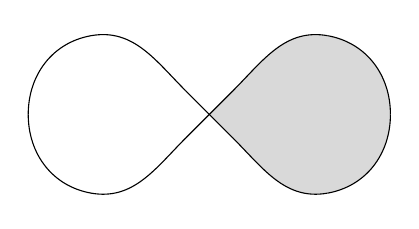
\begin{tikzpicture}[scale=1]
              \tikzset{->-/.style={decoration={ markings,
                      mark=at position #1 with {\arrow[scale=2,>=stealth]{>}}},
                      postaction={decorate}}}
 \begin{scope} 
     \clip (0,0) to (0.3,0.3) to[in=170,out=45] (1.5,1) to[in=90,out=350] (2.3,0) to[in=10,out=270] (1.5,-1)to[in=315,out=190] (0.3,-0.3) to
     (0,0) ;
\clip[preaction={draw,fill=gray!30}] (-2,-2) rectangle (8,8);
                             \end{scope}
                             
    \draw [black] (-1.5,1) to[in=90,out=190] (-2.3,0);
    \draw [black] (-1.5,1) to[in=135,out=10] (-0.3,0.3);         
    \draw [black]  (-1.5,-1)to[in=270,out=170] (-2.3,0);
    \draw [black] (-1.5,-1)to[in=225,out=350] (-0.3,-0.3)  ;
    
    \draw [black] (1.5,1) to[in=90,out=350] (2.3,0);
    \draw [black] (1.5,1) to[in=45,out=170] (0.3,0.3);         
    \draw [black]  (1.5,-1)to[in=270,out=10] (2.3,0);
    \draw [black] (1.5,-1)to[in=315,out=190] (0.3,-0.3)  ;

    \draw [black] (-0.3,0.3) to (0.3,-0.3);
    \draw [black] (-0.3,-0.3) to (0.3,0.3);
\end{tikzpicture}
    \caption{Computation of $\t$ for the Legendrian unknot, the disk drawn lies in a $(n-1)$-dimensional family that sweeps the filling once.}
    \label{unknot}
\end{figure}

The Koszul complex is generated over $\mathbb{K}$ by $a^{k}$, $a^{k}c$ for $k \geq 0$.
We can compute the non-trivial part of the differential to be:
\[ d^\t(a^{k}c ) = a^{k+1}, \ \ \text{for all } k \geq 0 \]
hence $\t$ is acyclic. This is consistent with the classical Koszul duality between the algebras $C^*(S^n)$ and $C_{-*}(\Omega S^n)$
for $n>1$. 

Consider next the case when $L$ is decorated by $+$. Since $S^{n-1}$ is simply connected $CE^{\ast}(\Lambda)\approx CE^{\ast}_{\parallel}(\Lambda)$ and we will use the parallel copies version in our calculation. Choose a Morse function on $\Lambda$ with a single minimum and a single maximum. Denote the corresponding Reeb chords $x$ (the co-unit chord) and $y$. Then
\[ 
LC_{\ast}^{\parallel}(\Lambda)= 
\mathbb{K}\cdot x \oplus \mathbb{K}\cdot y\oplus \mathbb{K} \cdot c, \ \ |x|=0,\;|y|=-(n-1),\;|c|=-n. 
\]
Here 
\[ 
\Delta_{1}(c)=y,\quad \Delta_{2}(x)=x\otimes x + +(-1)^{n-1}x\otimes y + y\otimes x + (-1)^{n}x\otimes c + c\otimes x,
\]
and all other operations are trivial. It follows that
\[ 
CE^{\ast}_{\parallel}(\Lambda)=\Omega(LC_{\ast}^{\parallel}(\Lambda)) \simeq \mathbb{K}.
\]
This is in line with Conjecture \ref{conjintro} which says that
$CE^{\ast}(\Lambda)\simeq CE^{\ast}_{\parallel}(\Lambda)$ is isomorphic to $CW^{\ast}(C)$, where $C$ is the cotangent fiber in the manifold obtained by attaching a cotangent end $T^{\ast}(S^{n-1}\times[0,\infty))$ to the ball along $\Lambda$. The manifold that results from this attachment is simply $T^{\ast}\R^{n}$ and the wrapped Floer cohomology of the cotangent fiber $C$ has rank 1 and is generated by the minimum in the disk $C$, in accordance with the above calculations.

Finally, the twisting co-chain $\t$ in the $+$ case is the canonical map $\K\to\K$, and again the
Koszul complex is acyclic. As explained in Section \ref{Sec:LegLag} this map is induced by a map
$\t'\colon LC_{\ast}^{\parallel}(\Lambda)\to (\Bar{CF^{\ast}(L)})^{\#}$. To define $CF^{\ast}(L)$ we use a Morse function on $L$ with a single local minimum and which is increasing in the end corresponding to a shift in the positive Reeb direction. Denote the generator of $CF^{\ast}(L)$ corresponding to the minimum $u$, $|u|=0$. Then  
\[ 
\t'(x)=u',
\] 
where $u'$ is the dual of $u$ and the holomorphic strip is the thin strip corresponding to a rigid Morse flow line from the minimum $u$ to the minimum $y$ in the boundary.  
\subsubsection{Geometric twisting cochain for the Hopf link}
\begin{figure}[h!]
	\centering
	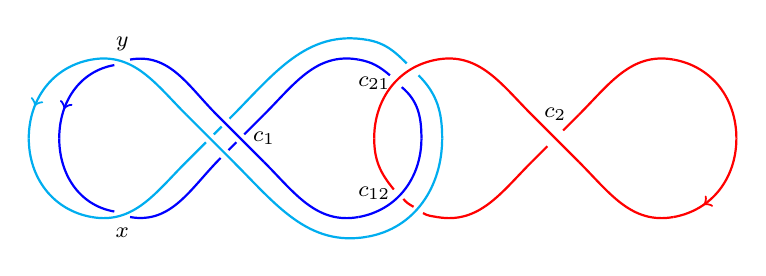
\begin{tikzpicture}[scale=1]
	%  \tikzset{->-/.style={decoration={ markings,
	%             mark=at position #1 with {\arrow[scale=2,>=stealth]{>}}},
	%            postaction={decorate}}}
	
	
	\tikzset{->-/.style={decoration={ markings,
				mark=at position #1 with {\arrow{>}}},postaction={decorate}}}
	
	\draw [blue, thick=1.5, ->-=.7] (-1.6,0.93) to[in=90,out=190] (-2.3,0);
	\draw [blue, thick=1.5] (-1.4,1) to[in=135,out=10] (-0.3,0.3);         
	\draw [blue, thick=1.5]  (-1.6,-0.93)to[in=270,out=170] (-2.3,0);
	\draw [blue, thick=1.5] (-1.4,-1)to[in=225,out=350] (-0.25,-0.25)  ;
	
	\draw [blue, thick=1.5] (1.5,1) to[in=45,out=170] (0.3,0.3);         
	
	\draw [blue, thick=1.5]  (1.5,-1)to[in=270,out=10] (2.3,0);
	\draw [blue, thick=1.5] (1.5,1) to[in=140,out=350] (1.9,0.8);
	\draw [blue, thick=1.5] (2.05,0.65) to[in=90,out=320] (2.3,0);
	
	
	\draw [blue, thick=1.5] (1.5,-1)to[in=315,out=190] (0.3,-0.3)  ;
	
	\draw [blue, thick=1.5] (-0.3,0.3) to (0.3,-0.3);
	\draw [blue, thick=1.5] (-0.15,-0.15) to (-0.05,-0.05);
	\draw [blue, thick=1.5] (0.05,0.05) to (0.3,0.3);
	
	
	\begin{scope}[xshift=-11]
	\draw [cyan, thick=1.5, ->-=.7] (-1.5,1) to[in=90,out=190] (-2.3,0);
	\draw [cyan, thick=1.5] (-1.5,1) to[in=135,out=10] (-0.3,0.3);         
	\draw [cyan, thick=1.5]  (-1.5,-1)to[in=270,out=170] (-2.3,0);
	\draw [cyan, thick=1.5] (-1.5,-1)to[in=225,out=350] (-0.3,-0.3)  ;
	
	\draw [cyan, thick=1.5] (2,1.25) to[in=45,out=170] (0.25,0.25);         
	
	\draw [cyan, thick=1.5]  (2,-1.25)to[in=270,out=10] (2.95,0);
	\draw [cyan, thick=1.5] (2,1.25) to[in=135,out=350] (2.5,0.95);
	\draw [cyan, thick=1.5] (2.65,0.8) to[in=90,out=315] (2.95,0);
	
	
	\draw [cyan, thick=1.5] (2,-1.25)to[in=315,out=190] (0.3,-0.3)  ;
	
	\draw [cyan, thick=1.5] (-0.3,0.3) to (0.3,-0.3);
	\draw [cyan, thick=1.5] (-0.3,-0.3) to (-0.05,-0.05);
	\draw [cyan, thick=1.5] (0.05,0.05) to (0.15,0.15);
	
	\end{scope} 
	
	
	\draw [red, thick=1.5] (2.5,1) to[in=90,out=190] (1.7,0);
	
	\draw [red, thick=1.5] (2.5,-1) to[in=330,out=170] (2.32,-0.95);
	\draw [red, thick=1.5] (2.2,-0.87) to[in=310,out=150] (2.07,-0.77);
	
	\draw [red, thick=1.5] (1.95,-0.65) to[in=270,out=130] (1.7,0);
	
	
	\draw [red, thick=1.5] (2.5,1) to[in=135,out=10] (3.7,0.3);         
	\draw [red, thick=1.5] (2.5,-1)to[in=225,out=350] (3.7,-0.3)  ;
	
	\draw [red, thick=1.5] (5.5,1) to[in=90,out=350] (6.3,0);
	\draw [red, thick=1.5] (5.5,1) to[in=45,out=170] (4.3,0.3);         
	\draw [red, thick=1.5, ->-=.7]  (6.3,0)to[in=10,out=270] (5.5,-1);
	\draw [red, thick=1.5] (5.5,-1)to[in=315,out=190] (4.3,-0.3)  ;
	
	\draw [red, thick=1.5] (3.7,0.3) to (4.3,-0.3);
	\draw [red, thick=1.5] (3.7,-0.3) to (3.9,-0.1);
	\draw [red, thick=1.5] (4.1,0.1) to (4.3,0.3);
	
	\node at (0.3,0) {\footnotesize{$c_1$}}; 
	\node at (1.7,0.7) {\footnotesize{$c_{21}$}}; 
	\node at (1.7,-0.7) {\footnotesize{$c_{12}$}}; 
	\node at (4,0.3) {\footnotesize{$c_2$}}; 
	\node at (-1.5,1.2) {\footnotesize{$y$}}; 
	\node at (-1.5,-1.2) {\footnotesize{$x$}}; 
	
	\end{tikzpicture}
	\caption{Hopf link with one (blue) marked $+$ and one (red) marked $-$ components.}
	\label{hopfparallel}
\end{figure}

In this section we carry out the geometric calculation of the twisting cochain for the Hopf link. As
explained we cannot directly calculate the twisting cochain into the Legendrian coalgebra with
coefficients in chains of the based loop space. We can however calculate the corresponding twisting
cochain when we replace chains on the based loop space with the Morse theory of parallel copies for
the components decorated by a positive sign. To carry out the calculation we pick a Morse function
on the component $\Lambda^{+}$ with on minimum $x$ and a maximum $y$. We place them on the circle
and choose parallel copies as shown in Figure \ref{hopfparallel}. The parallel copies algebra $CE_{\parallel}^{\ast}(\Lambda)$ is
\[ 
\k\langle x,y,c_{1},c_{12},c_{21},c_{2}\rangle,
\]
where we use notation for Reeb chords and Floer cohomology generators as in Section \ref{ssec:Hopflink}. The differential is
\begin{align*}
d c_{1} &= xc_{1} + c_{1}x + y + c_{12}c_{21},\\
d x &= xx,\\
dy &= xy - yx,\\
dc_{12} &= -xc_{12},\\
dc_{21} &= c_{21}x,\\
dc_{2} &= c_{21}c_{12}.
\end{align*}
Passing to $CE^{\ast}_{\parallel}(\Lambda)$ means dividing out by the cokernel of the coaugmentation that takes $e_{1}$ to $x$. This gives the algebra
\[ 
\k\langle y,c_{1},c_{12},c_{21},c_{2}\rangle,
\]
and the differential becomes
\begin{align*}
d c_{1} &= y + c_{12}c_{21},\\
dc_{2} &= c_{21}c_{12}.
\end{align*}

The twisting cochain $\t$ is induced from a map $\t'\colon LC_{\ast}^{\parallel}(\Lambda)\to (\Bar(\k_{-}\oplus CF^{\ast}(L)))^{\#}$ that counts holomorphic disks with one positive puncture and boundary on $L$, and with several punctures at Lagrangian intersection points in the compact part, see \eqref{eq:deft'}. In the current example it is straightforward to find these disk. Note first that by general properties, see Proposition \ref{twch},
\[ 
\t'(x)=a_{1}^{\vee},
\]
where $a_{1}$ is the idempotent corresponding to the minimum of the shifting Morse function on $L_{1}$. The holomorphic disk corresponds to a Morse flow line connecting $x$ to $u_{1}$.  We next consider $\t'(c_{1})$ and $\t'(c_{2})$. Consider first the moduli spaces $\mathcal{M}^{\fl}(c_{j})$ of holomorphic disks with a positive puncture at $c_{j}$ and boundary on $L_{j}$. As in the case of the unknot this moduli space sweeps $L_{j}$. On both $L_{1}$ and $L_{2}$ the shifting functions have one critical point, on $L_{1}$
it is a minimum and on $L_{2}$ a maximum. The maximum is constraining for the map into the linear dual of $CF^{\ast}(L_{j})$, whereas the minimum is not. We find that
\[ 
\t'(c_{1})=0,\quad \t'(c_{2})= a_{2}^{\vee}.
\] 

The space $\mathcal{M}^{\fl}(c_{j})$ give further information of the twisting co-chain as follows. Note that as the evaluation map hits the double point one can glue on a constant disk. These broken disks are also the boundary of the 1-dimensional moduli spaces $\mathcal{M}^{\fl}(c_{1}a_{12}a_{21})$ and $\mathcal{M}^{\fl}(c_{2}a_{21}a_{12})$. The other end of these moduli spaces correspond to broken disks with one level in the symplectization, a disk in $\mathcal{M}^{\sy}(c_{1}c_{12}c_{21})$ in the former case and in $\mathcal{M}^{\sy}(c_{2}c_{21}c_{12})$ in the latter, and two disks one in $\mathcal{M}^{\fl}(c_{12}a_{12})$ and one in $\mathcal{M}^{\fl}(c_{21}a_{21})$ attached at its negative end. The last disks contribute to $\t'$ and we conclude that
\[ 
\t'(c_{12})=a_{12}^{\vee},\quad \t'(c_{21})=a_{21}^{\vee}.
\]
Finally, we compute $\t'(y)$. Since $y$ is a small chord corresponding to a critical point at infinity of the shifting Morse function the only contributions to $\t'(y)$ comes from small holomorphic disks that are controlled by the Morse theory. It is straightforward to check that the only rigid disk corresponds to a flow line in $L_{1}$ connecting $y$ to the intersection point and that this flow line corresponds to a holomorphic triangle in $\mathcal{M}^{\fl}(ya_{12}a_{21})$. It follows that
\[ 
\t'(y)=a_{21}^{\vee}a_{12}^{\vee}.
\] 

The actual twisting co-chain takes the cokernel $\overline{LC}_{\ast}(\Lambda)$ of the co-augmentation into the cokernel of the co-units. Concretely, this means disregarding $x$ and $a_{1}^{\vee}$, and we get
\[ 
\t(c_{1})=0,\;\t(c_{2})=a_{2}^{\vee},\;\t(c_{12})=a_{12}^{\vee},\;\t(c_{21})=a_{21}^{\vee},
\;\t(y)=a_{12}^{\vee}a_{21}^{\vee}.
\]


\begin{rem}
	We point out that the parallel copies algebra $CE_{\parallel}^{\ast}(\Lambda)$ is defined using a fixed augmentation (in the current example the zero augmentation) on the one copy version of $CE^{\ast}(\Lambda)$. Here this is reflected in the change of variables $t-e_{1}=y$.
\end{rem}

\subsubsection{Products of spheres}
We will consider a Legendrian embedding $\Lambda\subset\R^{2(m+k)-1}$, where the ambient space is
standard contact $(2(m-k)-1)$-space with coordinates $(x,y,z)\in\R^{m+k-1}\times\R^{m+k-1}\times\R$
and contact form $dz-y\cdot dx$. We will define it by describing its front in $\R^{m+k-1}\times\R$.
To this end consider first the following construction of the front of the Legendrian unknot in
$\R^{n}\times\R$. Take a disk $D^{n}$ lying in $\R^n$. Think of it as having multiplicity two and
lift one of the sheets up in the auxiliary $\R$-direction (with coordinate $z$) keeping it fixed
along the boundary. In this way we construct the front of the standard unknot with Reeb chord at the maximum distance between the two sheets and a cusp edge along the boundary of $D^{n}$. Consider now instead the base $\R^{m+k-1}$ and the standard embedding of the $k$-dimensional sphere $S^{k}$ into this space. A tubular neighborhood of this embedding has the form $S^{k}\times D^{m-1}$ with fibers $D^{m-1}$. Now take two copies of this tubular neighborhood and repeat the above construction for the $D^{m-1}$ in each fiber. The result is the front of a Legendrian $S^{k}\times S^{m-1}$ with an $S^k$ Bott-family of Reeb chords corresponding to the maxima in fibers. Figure \ref{prodsphere} shows this front after Morse perturbation. The resulting Legendrian $\Lambda$ has only two Reeb chords. We denote them $a$ of grading $|a|=-(m+k)$ and $b$ of grading $|b|=-m$. Note also that $\Lambda$ has an exact Lagrangian filling $L\approx D^{m}\times S^{k}$.
 
\begin{figure}[h!]
    \centering
    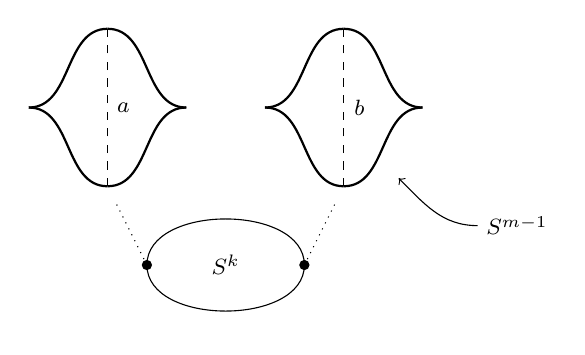
\begin{tikzpicture}[scale=1]

    \tikzset{->-/.style={decoration={ markings,
                mark=at position #1 with {\arrow{>}}},postaction={decorate}}}

  %      \begin{scope} [scale=0.6, yshift =-5cm] 
  %      \draw [black, ->-=1] (0,0) to (0,1);
  %      \node at (0.2,1.1) {\footnotesize{$z$}};
  %      \draw[black, ->-=1] (0,0) to (1,0);
  %      \node at (1.8,0) {\footnotesize{$x_{m+k-1}$}};
  %      \draw[black, ->-=1] (0,0) to (-0.55,-0.55);
 %       \node at (-0.75,-0.75) {\footnotesize{$x_1$}};
 %       \end{scope}

        \begin{scope} 

            \draw[black, thick=1] (0,0) to[in=180,out=0] (1,1); 
            \draw[black, thick=1] (2,0) to[in=0,out=180] (1,1); 
 \draw[black, thick=1] (0,0) to[in=180,out=0] (1,-1); 
 \draw[black, thick=1] (2,0) to[in=0,out=180] (1,-1); 

       \draw[black, dashed] (1,-1) to (1,1); 
       \node at (1.2, 0) {\footnotesize{$a$}}; 
        \end{scope}        


        \begin{scope} [xshift=3cm] 

            \draw[black, thick=1] (0,0) to[in=180,out=0] (1,1); 
            \draw[black, thick=1] (2,0) to[in=0,out=180] (1,1); 
 \draw[black, thick=1] (0,0) to[in=180,out=0] (1,-1); 
 \draw[black, thick=1] (2,0) to[in=0,out=180] (1,-1); 
   \draw[black, dashed] (1,-1) to (1,1); 
       \node at (1.2, 0) {\footnotesize{$b$}}; 
    
       \draw[black, ->-=1 ] (2.7,-1.5) to[in=315, out=180] (1.7,-0.9); 
        \node at (3.2, -1.5) {\footnotesize $S^{m-1}$};
        \end{scope}        

        \begin{scope} [xshift=1.5cm, yshift=-2cm] 

      \draw[thick, fill=black, scale=5] (0,0) circle(.01);
      \draw[thick, fill=black, scale=5] (0.4,0) circle(.01);

         \draw(0,0) to[in=90, out=90] (2,0);
         \draw(0,0) to[in=270, out=270] (2,0);
        \node at (1,0) {\footnotesize{$S^k$}}; 

            \draw[dotted] (0,0) to (-0.4,0.8); 
            \draw[dotted] (2,0) to (2.4,0.8); 


        \end{scope} 

\end{tikzpicture}
    \caption{Front of products of spheres}
    \label{prodsphere}
\end{figure}


Consider first the case when $L$ is decorated by $-$. If $d$ is the differential in 
$CE^{\ast}(\Lambda)$ we have
\[ 
da = 0,\; db=0.
\]
The Floer cohomology of $L$ is defined by choosing a shifting function which is decreasing at infinity and we find that $CF^{\ast}$ has two generators $M$, $|M|=m+k$ and $S$, $|S|=m$. As in the case of the unknot $\mathcal{M}^{\fl}(a)$ sweeps $L$ and $\mathcal{M}^{\fl}(b)$ sweeps $D^{m}\times \mathrm{pt}$. It follows that the twisting co-chain is
\[ 
\t(a)=M^{\vee},\; \t(b)=S^{\vee}
\] 
and duality holds.

Consider second the case when $L$ is decorated by $+$. In this case there are additional generators of $LC_{\ast}^{\parallel}(\Lambda)$ corresponding to the Morse theory of $\Lambda$. We have in addition to $a$ and $b$ above also
\[ 
x,\;|x|=0,\quad s_{1},\;|s_{1}|=-k,\quad  s_{2},\;|s_{2}|=-(m-1),\quad y,|y|=-(m+k-1).
\]
It follows that $CE^{\ast}_{\parallel}(\Lambda)$ is generated by $s_{1}$, $s_{2}$, $y$, $a$, and $b$. Using the flow tree description of moduli spaces $\mathcal{M}^{\sy}$ one verifies that if $d$ is the differential on $CE^{\ast}_{\parallel}(\Lambda)$ then
\begin{align*} 
d a &=y - ((-1)^{km}bs_{1}+s_{1}b),\; dy = s_{1}s_{2} + (-1)^{k(m-1)}s_{2}s_{1},\\
db &=s_{2},\; ds_{1}=0,\; ds_{2}=0.
\end{align*}

The Floer cohomology of $L$ is defined by choosing a shifting function which is increasing at
infinity and we find that $CF^{\ast}$ has two generators $M$, $|M|=0$ and $S$, $|S|=k$, where
$M$
is the unit. It follows that $(\Bar CF^{\ast}(L))^\# \simeq \Omega CF_{\ast}(L))$ is generated by
$S^{\vee}$ with $|S^{\vee}|=-k$ and the twisting co-chain is
\[ 
\t(a)=0,\; \t(y) = 0,\; \t(b)=0,\; \t(s_{2})=0,\;\t(s_{1})=S^{\vee},
\] 
and duality holds.

\subsubsection{Plumbings of simply-connected cotangent bundles} 

Let $\mathcal{T}$ be a tree with vertex set $\Gamma$. For each $v \in \Gamma$, let $M_v$ be a compact
simply-connected manifold of dimension $n \geq 3$. We will see that duality holds between
the wrapped and the compact Fukaya categories of the symplectic manifold $X_\mathcal{T}$
obtained by plumbing the collection of $T^*M_v$ according to the tree $\mathcal{T}$. As usual, we take the pre-surgery
perspective. Hence, consider a handle decomposition of each $M_v$ with a unique top-dimensional $n$-handle. Removing this handle, we get manifolds $L_v$ with spherical boundary $\Lambda_v$. Let
$W_{\mathcal{T}}$ be the subcritical
Weinstein manifold obtained by plumbing the cotangent bundles $T^*L_v$ according to the tree
$\mathcal{T}$. We take the plumbing region to be away from the boundary of $L_v$. Write $\Lambda =
\bigsqcup_v \Lambda_v$ for the Legendrian in the boundary of the subcritical Weinstein manifold
$W_\mathcal{T}$ which is filled by the Lagrangian $L=\bigcup_{v} L_{v}$.
Equip the components of $\Lambda$ with either $+$ or $-$ labeling. 

\begin{thm} \label{plumbs}  
	If $n \geq 3$ and $L_v$ is simply-connected for each $v\in\Gamma$, then $CE^*(\Lambda)$ and $CF^*(L)$ are Koszul dual. 
\end{thm}
\begin{proof} 
	Consider first the case $n \geq 5$. Pick a handle decomposition of $L_{v}$ without
    $1$- and $(n-1)$-handles. The existence of such a handle decomposition is equivalent to
    simply-connectivity in high dimensions by the work of Smale. Consider the corresponding
    Weinstein handle decomposition of $T^{\ast}L_{v}$.  Attaching a $k$-handle alters the Legendrian
    boundary by surgery and adds Reeb chords in the co-core sphere of the handle of grading $\le
    -(n-k)$ and it follows that all Reeb chords of $\Lambda_{v}$ have grading $\le -2$. To construct
    $\Lambda\subset \partial W_{\mathcal{T}}$, we perform a version of boundary connected sum as
    follows. For each edge in $\mathcal{T}$ we pick a $2n$-ball $B$ with two transversely
    intersecting Lagrangian disks $D\subset B$ that intersect the boundary sphere $\partial B$ in a
    standard Legendrian Hopf link $\Delta$. We then make boundary connected sum adding $(B,\Delta)$
    to join the $T^{\ast}L_{v}$ according to the tree. This adds Reeb chords of index $\le -(n-1)$
    in the boundary connected sum handles and further Reeb chords corresponding to the Reeb
    chords of each Hopf link, which effectively has four Reeb chords: two Reeb chords connecting the unknot components to themselves of grading $-n$ and two mixed Reeb chords connecting distinct components. We can pick gradings so that the gradings of these two mixed chords are $-d$ and
    $-(n-d)$ for any $d$, where the first Reeb chord goes from the component closest to priori fixed
    root of the tree $\mathcal{T}$ to the one further from it and the other in the opposite
    direction. Taking $d$ between $2$ and $n-2$ we find that $LC_*(\Lambda)$ is simply connected as is $\Lambda$. The result then follows from Theorem \ref{mainthm}.
    
For $n=4$, we can stabilize by multiplying by $\R^{N}$ as described in Remarks \ref{r:dim4} and \ref{r:dim4iso} to get 1-reduced versions of the Legendrian and Lagrangian algebras and then use the above argument.
         
Finally for $n=3$, the assumptions of Theorem \ref{mainthm} does not hold but we recall from
Remark \ref{locfinrem} that to apply the duality result from Theorem \ref{mainthm} all we really need is that $\Bar (LA^*)$ is locally finite. This is easily seen to be the case in our case, since the
    plumbing is according to a tree (which by definition has no cycles) and for any word of Reeb chords
    that do not consist of connecting Reeb chords going away from the root of the tree the
    grading has to increase with the size of the word. Alternatively, in this case we know by
    Perelman's theorem that we can take $\Lambda$ as a link of standard Legendrian spheres linked
    according to the tree as Hopf links and $\Bar (LA^*)$ can be seen to be locally finite directly. \end{proof}
\begin{rem}
	The case $n=2$ corresponds to plumbing of copies of $T^*S^2$. This case was studied in \cite{EtLe} and a
    version of the duality result still holds, at least when $\mathrm{char}(\mathbb{K}) =0$.
    However, the above argument fails in that case and a more complicated argument using an additional
    grading is used in \cite{EtLe}. Also a set of examples for $n=1$ are studied 
    in \cite{LePol}, where the plumbing tree is a star and the corresponding
    symplectic manifolds is a punctured torus. The duality still holds in this case, even though
    this is a plumbing of $T^*S^1$'s (not simply-connected). The proof of duality given in \cite{LePol} uses homological mirror symmetry. 
\end{rem}

\subsubsection{The trefoil} 

\begin{figure}[h!]
    \centering
    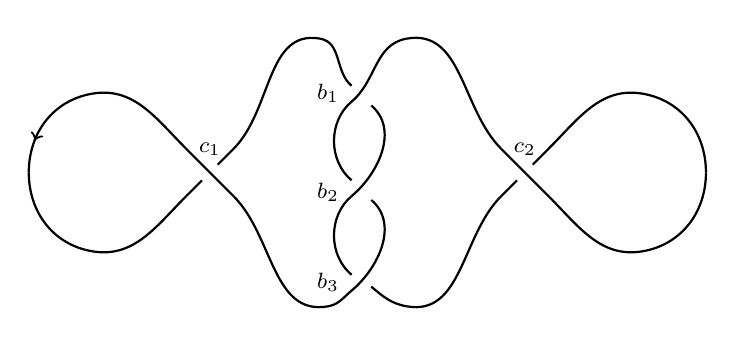
\begin{tikzpicture}[scale=1]

    \tikzset{->-/.style={decoration={ markings,
                mark=at position #1 with {\arrow{>}}},postaction={decorate}}}
            
\draw [black, thick=1, ->-=.7] (-1.5,1) to[in=90,out=190] (-2.3,0);
        \draw [black, thick=1] (-1.5,1) to[in=135,out=10] (-0.3,0.3);         
    \draw [black, thick=1]  (-1.5,-1)to[in=270,out=170] (-2.3,0);
    \draw [black, thick=1] (-1.5,-1)to[in=225,out=350] (-0.3,-0.3)  ;
    
    \draw [black, thick=1] (1.4,1.7) to[in=45,out=170] (0.3,0.3);         
       
    \draw [black, thick=1] (1.4,1.7) to[in=140,out=350] (1.8,1.1);
        \draw [black, thick=1] (2.05,0.85) to[in=40,out=320] (1.8,-0.3);
    \draw [black, thick=1] (2.05,-0.35) to[in=40,out=320] (1.8,-1.5);
 

     \draw [black, thick=1] (1.8,-1.5)to[in=10,out=220] (1.5,-1.7)  ;

 
    \draw [black, thick=1] (1.5,-1.7)to[in=315,out=190] (0.3,-0.3)  ;

    \draw [black, thick=1] (-0.3,0.3) to (0.3,-0.3);
    \draw [black, thick=1] (-0.3,-0.3) to (-0.1,-0.1);
    \draw [black, thick=1] (0.1,0.1) to (0.3,0.3);    
        
        \draw [black, thick=1] (2.5,1.7) to[in=40,out=190] (1.8,0.9);
        \draw [black, thick=1]  (1.8,0.9)to[in=140,out=220] (1.8,-0.1);
        \draw [black, thick=1]  (1.8,-0.3)to[in=140,out=220] (1.8,-1.3);

 \draw [black, thick=1]  (2.05,-1.45)to[in=170,out=320] (2.5,-1.7);

    \draw [black, thick=1] (2.5,1.7) to[in=135,out=10] (3.7,0.3);         
    \draw [black, thick=1] (2.5,-1.7)to[in=225,out=350] (3.7,-0.3)  ;
    
    \draw [black, thick=1] (5.5,1) to[in=90,out=350] (6.3,0);
    \draw [black, thick=1] (5.5,1) to[in=45,out=170] (4.3,0.3);         
    \draw [black, thick=1]  (6.3,0)to[in=10,out=270] (5.5,-1);
    \draw [black, thick=1] (5.5,-1)to[in=315,out=190] (4.3,-0.3)  ;

    \draw [black, thick=1] (3.7,0.3) to (4.3,-0.3);
    \draw [black, thick=1] (3.7,-0.3) to (3.9,-0.1);
    \draw [black, thick=1] (4.1,0.1) to (4.3,0.3);

    \node at (0,0.3) {\footnotesize{$c_1$}}; 
    
    \node at (1.5,1) {\footnotesize{$b_{1}$}}; 
    \node at (1.5,-0.25) {\footnotesize{$b_{2}$}}; 
    \node at (1.5,-1.4) {\footnotesize{$b_{3}$}}; 
    
    \node at (4,0.3) {\footnotesize{$c_2$}}; 

    \end{tikzpicture}
    \caption{Trefoil }
    \label{trefoil}
\end{figure}




Consider the standard Legendrian trefoil $\Lambda \subset S^{3}$ described in Figure
\ref{trefoil}. Let us first consider the case when $\Lambda$ is marked $-$. With respect to the standard choice of orientation datum, the
Chekanov-Eliashberg DG-algebra $CE^{\ast}$ is then given by the free algebra
\[ \mathbb{K} \langle c_1, c_2, b_1,b_2,b_3 \rangle, \ \ |c_1|=|c_2|=-1, |b_{1}|=|b_{2}|=|b_{3}|=0 \]
and the non-trivial part of the differential can be read from Figure \ref{trefoil} as follows: 
\begin{align*}
    dc_1 &= 1 + b_{1} + b_{3} + b_{3}b_{2}b_{1} \\
    dc_2 &=-1 - b_{1} - b_{3} - b_{1}b_{2}b_{3}. 
\end{align*}

It is well known that $\Lambda$ has an exact Lagrangian torus filling. (In fact, there are at least
five of them, see \cite{EKH}).  Any of these can be obtained by doing surgery (pinch move) at
$b_1$, $b_2$ and $b_3$ in some order. Corresponding augmentations $\epsilon_L\colon CE^* \to \K$ are given by their values
$\epsilon(b_{1}), \epsilon(b_{2}), \epsilon(b_{3}) \in \K$ subject to the condition:
\[ 
1+ \epsilon(b_{1}) + \epsilon(b_{3}) + \epsilon(b_{1}) \epsilon(b_{2}) \epsilon(b_{3})  =0.   
\]

Note that since $CE^*$ is not simply-connected, Theorem \ref{mainthm} does not apply 
here. In fact, duality does not hold in this example. However, Theorem
\ref{comple} shows that there is a quasi-isomorphisms of completions  
\[
\widehat{CE}^* \cong \widehat{\Omega} C_*(T^2) \cong \K [[u, v]] 
\] 
where the latter is a power series ring in two commuting variables concentrated in degree 0. 

Thus, the completion map composed with the twisting cochain gives an algebra map: 
\[ 
H^0(CE^*) = \K \langle b_{1},b_{2},b_{3} \rangle / \langle 1+b_{1}+b_{3}+b_{3}b_{2}b_{1} ,
1+b_{1}+b_{3}+b_{1}b_{2}b_{3} \rangle   \to \K[[u,v]]. \] 
We claim that this map is injective. Indeed, observe that $H^0(CE^*)$ is a commutative
algebra: 
\[ 
d( c_1 + c_2 + b_{3}b_{2} c_1 + c_1 b_{2}b_{3}) = b_{3}b_{2} - b_{2}b_{3}, 
\]
and thus, $b_{2}$ commutes with $b_{3}$ in homology. Using this, one shows similarly that $b_{1}$ commutes with $b_{2}$ and $b_{3}$, see \cite{CaMu}. 
Hence, we have a completion map from a commutative ring to its completion
\[ 
H^0(CE^*) = \K [b_{1},b_{2},b_{3}] / (1+b_{1}+b_{3}+b_{1}b_{2}b_{3}) \to \K[[u,v]]. 
\]
It is a well known theorem, known as Krull intersection theorem, 
in commutative algebra that for any commutative Noetherian ring which is an
integral domain the completion map is injective. Thus, even though duality fails in this example, partial information can still be obtained by considering completions.

We next describe the twisting cochain $\t\colon LC_{\ast}(\Lambda)\to \Bar CF^{\ast}(L)^{\#}$ for one of the Lagrangian fillings $L$ of $\Lambda$. More precisely, we choose the filling which is obtained by pinching first at $b_{1}$, then at $b_{2}$, then at $b_{3}$, and finally filling the resulting unknots with Lagrangian disks, see \cite[Section 8.1]{EKH}. We think of the Lagrangian filling in as two disks connected by three twisted bands corresponding to the three pinchings. We next consider moduli spaces of holomorphic disks with boundary in $L$. Here \cite[Sections 4 and 5]{EKH} gives a description in terms of Morse flow trees which gives the following:
\begin{itemize}
\item $\mathcal{M}^{\fl}(b_{1})$ consists of one disk, $\delta_{1}^{1}$. 
\item $\mathcal{M}^{\fl}(b_{2})$ consists of two disks, $\delta_{2}^{1}$ and $\delta_{2}^{2}$.
\item $\mathcal{M}^{\fl}(b_{3})$ consists of two disks, $\delta_{3}^{1}$ and $\delta_{3}^{2}$
\end{itemize}
The boundaries of these disks are as follows.
\begin{itemize}
	\item $\partial \delta_{1}^{1}$ is fiber in the first twisted band.
	\item $\partial \delta_{2}^{1}$ is a fiber in the second twisted band, and $\partial \delta_{2}^{2}$ runs across the first and the second twisted band.
	\item $\partial\delta_{3}^{1}$ is a fiber in the third twisted band, and $\partial \delta_{3}^{2}$ runs across the second and the third twisted bands.
\end{itemize}
We next describe the moduli spaces $\mathcal{M}^{\fl}(c_{2})$, $\mathcal{M}^{\fl}(c_{1})$
in a completely analogous manner. The space has four components, all diffeomorphic to intervals, as follows:
\begin{itemize}
\item $\theta_{1}$ with one boundary point the disk in
    $\mathcal{M}^{\sy}(c_{2}b_{1})$ with $\delta_{1}^{1}$ attached, and the other the disk in
        $\mathcal{M}^{\sy}(c_{2}b_{1}b_{2}b_{3})$ with $\delta_{1}^{1}$, $\delta_{2}^{1}$, and $\delta_{3}^{2}$ attached.
\item $\theta_{2}$ with one boundary point the disk in
    $\mathcal{M}^{\sy}(c_{2}b_{3})$ with $\delta_{3}^{1}$ attached, and the other the disk in
        $\mathcal{M}^{\sy}(c_{2}b_{1}b_{2}b_{3})$ with $\delta_{1}^{1}$, $\delta_{2}^{2}$, and $\delta_{3}^{1}$ attached.
\item $\theta_{3}$ with one boundary point the disk in
    $\mathcal{M}^{\sy}(c_{2}b_{3})$ with $\delta_{3}^{2}$ attached, and the other the disk in
        $\mathcal{M}^{\sy}(c_{2}b_{1}b_{2}b_{3})$ with $\delta_{1}^{1}$, $\delta_{2}^{2}$, and $\delta_{3}^{2}$ attached.
\item $\theta_{4}$ with one boundary point the disk in $\mathcal{M}^{\sy}(c_{2})$ and the other the
    disk in $\mathcal{M}^{\sy}(c_{2}b_{1}b_{2}b_{3})$ with $\delta_{1}^{1}$, $\delta_{2}^{1}$, and $\delta_{3}^{1}$ attached.
\end{itemize}
Here the disks in $\theta_{4}$ sweeps the right hand disk of $L$, whereas the evaluation maps of
$\theta_{j}$, $1\le j\le 3$ does not map surjectively onto either disk. The moduli space
$\mathcal{M}^{\fl}(c_{1})$ also has four components only one of which sweeps the left hand disk of $L$.

In order to compute the Floer cohomology $CF^{\ast}(L)$ we pick a Morse function with one maximum $M$ and two saddle points $S_{1}$ and $S_{2}$. Letting the maximum lie in the right hand disk we find:
\[ 
\t(c_{1})=0,
\]
since the only way to rigidify a disk of dimension one is that its boundary passes the maximum $M$.

The twisting cochain can now in principle be computed from the moduli spaces $\mathcal{M}^{\fl}$ described above by attaching flow trees. To get an algebraically feasible twisting co-chain we first arrange the perturbation scheme so that 
\[ 
\t(b_{1})= S_{1}^{\vee}+S_{1}^{\vee}S_{2}^{\vee},
\] 
where the first term is $\delta_{1}^{1}$ with a flow line and the second with a flow tree, and next so that
\[ 
/\t(b_{3})= -S_{1}^{\vee},
\] 
the disk $\delta_{2}^{2}$ with a flow line contributes, other contributions cancel (the disk $\delta_{2}^{2}$ with two flow lines and the same disk with a flow tree, the two distinct disks with one flow lines). Remaining parts of the twisting cochain are now determined from the co-product in the Floer homology:
\[ 
dM^{\vee}= S_{1}^{\vee}S_{2}^{\vee}-S_{2}^{\vee}S_{1}^{\vee},
\]
the twisting cochain equation, and the sweeping property of $\theta_{4}$, as follows: 
\[ 
\t(c_{2})=M^{\vee}\left(\frac{1+S_{1}^{\vee}}{1+S_{1}^{\vee}+S_{1}^{\vee}S_{2}^{\vee}}\right) .
\] 
and
\[ 
\t(b_{2})= \frac{S_{2}^{\vee}}{(1+S_1^{\vee}+S_{1}^{\vee}S_{2}^{\vee})}.
\]
It is possible to check that these power series agree with the geometric count. We leave out the
details but describe the mechanism. In order to arrange that only one flow line can be attached to
$\delta_{1}^{1}$ we order the stable manifolds of the flow line of the parallel copies so that if a
flow line (or flow tree) between copy $j$ and $j-l$ is attached then following $\delta_{1}^{1}$ we already passed all intersections with stable manifolds between copy $j-l$ and $k$ for $k<j-l$. Now, if the disk intersects the collection of stable manifolds in the opposite direction this means that we can jump down in all ways, which then gives the desired power series. 


We finish this section by a brief discussion of the case $L$ decorated by $+$ and parallel copies. As usual this introduces two extra generators in addition to the Reeb chords above in $LC_{\ast}$, $x$, $|x|=0$ and $y$, $|y|=-1$, where $x$ is the counit corresponding to the minimum of the shifting function and $y$ is the maximum. In the reduced coalgebra (disregarding $x$) we get the new differential (using the augmentation $\epsilon_{L}$ above to change coordinates): 
\begin{align*}
dc_1 &= b_{1} + b_{3} - b_{3}b_{2}+b_{3}b_{2}b_{1} \\
dc_2 &=-y - b_{1} - b_{3} +b_{2}b_{3} - b_{1}b_{2}b_{3}. 
\end{align*}
In this case $CF^{\ast}$ is defined instead by choosing a shifting function that increases at infinity, and $CF^{\ast}$ is generated by the unit $u$, $|u|=0$ and $s_{1}$, $s_{2}$ with $|s_{j}|=1$. The new twisting cochain is
\[ 
\t(c_{1})=\t(c_{2})=0,\; \t(y)= \left(s_{1}^{\vee}s_{2}^{\vee}-s_{2}^{\vee}s_{1}^{\vee}\right)\left(\frac{1+s_{1}^{\vee}}{1+s_{1}^{\vee}+s_{1}^{\vee}s_{2}^{\vee}}\right),
\]
and $\t(b_{j})$ is exactly as above, after the substitutions $s_{j}\to S_{j}$, $j=1,2$. 


\subsubsection{Mirror of $7_2$}\label{lenny}

We next discuss an example where Koszulity fails and also the completion map fails to be injective,
even though $CE^*$ is supported in non-positive degrees. This
example was shown to us by Lenhard Ng. 

\begin{figure}[h!]
    \centering
    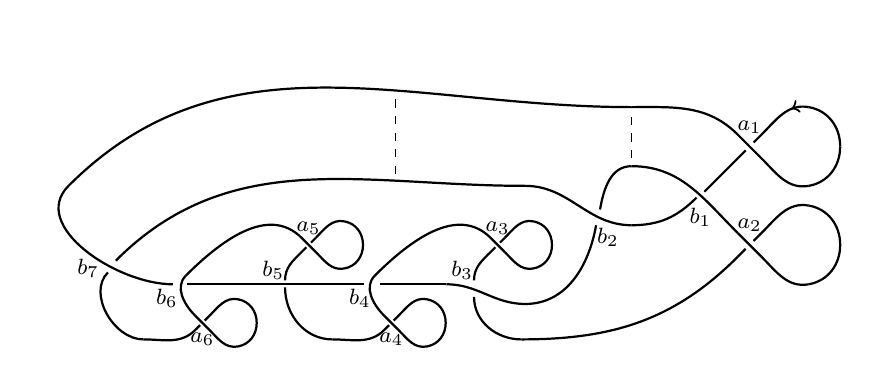
\begin{tikzpicture}[scale=1]
        %  \tikzset{->-/.style={decoration={ markings,
         %             mark=at position #1 with {\arrow[scale=2,>=stealth]{>}}},
          %            postaction={decorate}}}


    \tikzset{->-/.style={decoration={ markings,
                mark=at position #1 with {\arrow{>}}},postaction={decorate}}}
            

 \begin{scope}[scale=0.5, yshift=2.5cm]
    \draw [black, thick=1] (5.5,1) to[in=90,out=350] (6.3,0);
    \draw [black, thick=1, ->-=.3] (5.5,1) to[in=45,out=170] (4.3,0.3);         
    \draw [black, thick=1]  (6.3,0)to[in=10,out=270] (5.5,-1);
    \draw [black, thick=1] (5.5,-1)to[in=315,out=190] (4.3,-0.3)  ;

    \draw [black, thick=1] (3.7,0.3) to (4.3,-0.3);
    \draw [black, thick=1] (3.7,-0.3) to (3.9,-0.1);
    \draw [black, thick=1] (4.1,0.1) to (4.3,0.3);
  
    \node at (4,0.5) {\footnotesize{$a_1$}}; 
    
    \draw[black, thick=1] (3.7, 0.3) to[in=0 ,out=135] (1, 1);
   
    \draw[black, thick=1] (3.7, -0.3) to[in=45 ,out=225] (2.85, -1.15);
     \draw[black, thick=1] (2.65, -1.3) to[in=0 ,out=225] (1, -2);
     \node at (2.75, -1.8) {\footnotesize $b_1$}; 
     
    \draw[black, thick=1] (1, -2) to[in=0 ,out=180] (-1.7, -1);
   

 
    \end{scope}


    \begin{scope}[scale=0.5]
    \draw [black, thick=1] (5.5,1) to[in=90,out=350] (6.3,0);
    \draw [black, thick=1] (5.5,1) to[in=45,out=170] (4.3,0.3);         
    \draw [black, thick=1]  (6.3,0)to[in=10,out=270] (5.5,-1);
    \draw [black, thick=1] (5.5,-1)to[in=315,out=190] (4.3,-0.3)  ;

    \draw [black, thick=1] (3.7,0.3) to (4.3,-0.3);
    \draw [black, thick=1] (3.7,-0.3) to (3.9,-0.1);
    \draw [black, thick=1] (4.1,0.1) to (4.3,0.3);

    \node at (4,0.5) {\footnotesize{$a_2$}}; 
    

    \draw[black, thick=1] (3.7, 0.3) to[in=0 ,out=135] (1, 2);
    \draw[black, thick=1] (3.7, -0.3) to[in=0,out=225] (-1.8,-2.4);

    \draw[black, thick=1] (1, 2) to[in=80 ,out=180] (0.2, 0.9);
    \draw[black, thick=1] (0.1, 0.5) to[in=0 ,out=260] (-1.7, -1.5);
    \node at (0.4, 0.2) {\footnotesize $b_2$};  
        
    \draw[black, thick=1] (-1.7, -1.5) to[in=0 ,out=180] (-3.7, -1);
    
    \node at (-3.3,-0.65) {\footnotesize $b_3$}; 
    \draw[black, thick=1] (-3.7, -1) to[in=0 ,out=180] (-5.4, -1);
     \node at (-5.9,-1.35) {\footnotesize $b_4$}; 
    \draw[black, thick=1] (-5.8, -1) to[in=0 ,out=180] (-10.3, -1);
      \node at (-8.1,-0.65) {\footnotesize $b_5$}; 
    
    \node at (-10.8,-1.35) {\footnotesize $b_6$}; 

    \draw[black, thick=1] (-10.65, -1) to[in=225 ,out=180] (-13.3, 1.5);
    
    \draw[black, thick=1] (-11.4, -2.4) to[in=225 ,out=180] (-12.3, -0.7);
  
    \draw[black, thick=1] (-13.3, 1.5) to[in=180 ,out=45] (1, 3.5);
   
     \draw[black, thick=1] (-12.1, -0.4) to[in=180 ,out=45] (-1.7, 1.5);
  
     \node at (-12.8,-0.6) {\footnotesize $b_7$}; 

    \draw[black, dashed] (-5, 1.8) to (-5,3.7);
    \draw[black, dashed] (1, 2.2) to (1,3.5);


    \end{scope}


    \begin{scope}[scale=0.3, xshift=-8cm ]
    \draw [black, thick=1] (5.5,1) to[in=90,out=350] (6.3,0);
    \draw [black, thick=1] (5.5,1) to[in=45,out=170] (4.3,0.3);         
    \draw [black, thick=1]  (6.3,0)to[in=10,out=270] (5.5,-1);
    \draw [black, thick=1] (5.5,-1)to[in=315,out=190] (4.3,-0.3)  ;

     \node at (4,0.7) {\footnotesize{$a_3$}}; 
    

    \draw [black, thick=1] (3.7,0.3) to (4.3,-0.3);
    \draw [black, thick=1] (3.7,-0.3) to (3.9,-0.1);
    \draw [black, thick=1] (4.1,0.1) to (4.3,0.3);
    \draw [black, thick=1] (3.7,-0.3) to[in=90, out=225] (3, -1.5);
    \draw [black, thick=1] (3,-2.2) to[in=180, out=270] (5, -4);
    \end{scope} 

    \begin{scope}[scale=0.3, xshift=-16cm ]
    \draw [black, thick=1] (5.5,1) to[in=90,out=350] (6.3,0);
    \draw [black, thick=1] (5.5,1) to[in=45,out=170] (4.3,0.3);         
    \draw [black, thick=1]  (6.3,0)to[in=10,out=270] (5.5,-1);
    \draw [black, thick=1] (5.5,-1)to[in=315,out=190] (4.3,-0.3)  ;
 
  \node at (4,0.7) {\footnotesize{$a_5$}}; 
    
    \draw [black, thick=1] (3.7,0.3) to (4.3,-0.3);
    \draw [black, thick=1] (3.7,-0.3) to (3.9,-0.1);
    \draw [black, thick=1] (4.1,0.1) to (4.3,0.3);
    \draw [black, thick=1] (3.7,-0.3) to[in=90, out=225] (3, -1.5);
    \draw [black, thick=1] (3,-1.8) to[in=180, out=270] (5, -4);


    \end{scope} 


     \begin{scope}[scale=0.3, xshift=-12.5cm, yshift=-3.3cm]
    \draw [black, thick=1] (5.5,1) to[in=90,out=350] (6.3,0);
    \draw [black, thick=1] (5.5,1) to[in=45,out=170] (4.3,0.3);         
    \draw [black, thick=1]  (6.3,0)to[in=10,out=270] (5.5,-1);
    \draw [black, thick=1] (5.5,-1)to[in=315,out=190] (4.3,-0.3)  ;

  \node at (4,-0.7) {\footnotesize{$a_4$}}; 
    
    \draw [black, thick=1] (3.7,0.3) to (4.3,-0.3);
    \draw [black, thick=1] (3.7,-0.3) to (3.9,-0.1);
    \draw [black, thick=1] (4.1,0.1) to (4.3,0.3);
    \draw [black, thick=1] (3.7,-0.3) to[in=0, out=225] (1.5, -0.7);
    
    \draw[black,thick=1] (3.7,0.3) to[in=225, out=135](3.3, 2);  
    \draw[black,thick=1] (3.3,2) to[in=135, out=45](8.2, 3.6);  
     
    \end{scope} 

 \begin{scope}[scale=0.3, xshift=-20.5cm, yshift=-3.3cm]
    \draw [black, thick=1] (5.5,1) to[in=90,out=350] (6.3,0);
    \draw [black, thick=1] (5.5,1) to[in=45,out=170] (4.3,0.3);         
    \draw [black, thick=1]  (6.3,0)to[in=10,out=270] (5.5,-1);
    \draw [black, thick=1] (5.5,-1)to[in=315,out=190] (4.3,-0.3)  ;

  \node at (4,-0.7) {\footnotesize{$a_6$}}; 
    
    \draw [black, thick=1] (3.7,0.3) to (4.3,-0.3);
    \draw [black, thick=1] (3.7,-0.3) to (3.9,-0.1);
    \draw [black, thick=1] (4.1,0.1) to (4.3,0.3);
    \draw [black, thick=1] (3.7,-0.3) to[in=0, out=225] (1.5, -0.7);
    
    \draw[black,thick=1] (3.7,0.3) to[in=225, out=135](3.3, 2);  
    \draw[black,thick=1] (3.3,2) to[in=135, out=45](8.2, 3.6);  
     
    \end{scope} 





   
    \end{tikzpicture}
    \caption{Mirror of $7_2$}
    \label{ngknot}
\end{figure}

Consider the Legendrian knot $\Lambda$ drawn in Figure \ref{ngknot} decorated $-$. It is easy to see
that two pinch moves indicated by dashed lines in the Figure \ref{ngknot} gives a Legendrian
unknot, hence $\Lambda$ has a Lagrangian torus filling, call it $L$. Thus, we again have a
completion map:
\[ H^0(CE^*) \to \K [[u, v]] \]
where $K[[u,v]]$ is the commutative powerseries algebra in two variables.

$CE^*$ is given by the free algebra:
\[ \K \langle a_1, a_2, a_3, a_4, a_5, a_6, b_1 ,b_2, b_3, b_4, b_5,b_6, b_7 \rangle ,
|a_i|=-1, |b_i| =0 \]
The differential is given by 
\begin{align*}
    da_1 &= -1 + (1+b_1 b_2)b_7 + b_1(1+b_4b_3) (1+b_6 b_5) \\
    da_2 &= 1- b_3(1+ b_2b_1) \\
    da_3 &= 1+ b_3b_4 \\
    da_4 &= 1+ b_5 b_4 \\
    da_5 &= 1+ b_5 b_6 \\
    da_6 &= 1+ b_7 b_6 
\end{align*}

Taking the quotient of $H^0(CE^*)$ by letting $b_4=b_6$, $b_3=b_5=b_7$, $b_1=1$ and $b_2=-1-b_4$
gives
\[ \langle  b_3, b_4 \rangle / \langle 1+ b_3b_4 \rangle \]
which is a non-commutative algebra.

Thus, the completion map cannot be injective in this case. Otherwise, $H^0(CE^*)$ and thus any
quotient of it would have been commutative. 


\subsection{Simply connected Legendrian submanifolds} 
Let $\Lambda\subset Y$ be a Legendrian
$(n-1)$-submanifold with $\pi_1(\Lambda)=1$ in the boundary $Y$ of a Weinstein $2n$-manifold $X$
that bounds an exact Lagrangian $L\subset X$. Assume that $c_{1}(X)=0$ and that the Maslov class of $L$ vanishes and that $L$ is relatively spin. Decorate $L$ by $-$. Our next result shows that if the symplectic homology of $X$ vanishes and if all Reeb
chords of $\Lambda$ have negative grading as generators of $CE^{\ast}(\Lambda)$ then $CE^{\ast}(\Lambda)$ is determined by the topology of $L$ and conversely. If $\Lambda$ is a sphere then we write $\overline{L}=L\cup_{\partial} D^{n}$ for
the closed manifold obtained by adding a disk to $L$ along $\Lambda$. 

\begin{thm} Suppose that $\Lambda =\Lambda^{-}$ is simply-connected. Assume that $SH^*(X)=0$ and that $CE^{\ast}(\Lambda)$ is supported in degrees $\le -1$. Then $L$ is simply connected. Moreover, if $\Lambda$ is a sphere then $CE^*(\Lambda)$ is isomorphic to $C_{-*}(\Omega \overline{L})$.
\end{thm}  

\begin{proof}
	Consider the wrapped Floer cohomology $HW_{\pi_1}^{\ast}(L)$ of $L$ with coefficients in $\Z[\pi_1(L)]$. Using our model for wrapped Floer cohomology in Section \ref{sec:CWnoHam}, a chain complex $CW_{\pi_{1}}^{\ast}(L)$ which calculates $HW_{\pi_{1}}^{\ast}(L)$ can be described as follows. Let $L=L_{0}$ and let $L_{1}$ be a parallel copy of $L$ shifted in the negative Reeb direction at infinity. The complex $CW_{\pi_{1}}^{\ast}(L)$ is then generated over $\Z[\pi_{1}]$ by the intersection points in $L_{0}\cap L_{1}$ which we call the Morse generators and the Reeb chords starting on $\Lambda_{0}$ and ending on $\Lambda_{1}$. The differential of a generator counts the usual rigid holomorphic strips, keeping track of the homotopy class of the loop obtained from the boundary component of the disk in $L_{1}$ completed by the reference paths connecting Reeb chord endpoints and intersection points to the base point. We point out that since there are no Reeb chords of degree $0$ the augmentation induced by $L$ is trivial and the high energy part of the differential on $CW^{\ast}_{\pi_{1}}$ counts honest holomorphic strips (without extra negative punctures at augmented Reeb chords).
	As for usual wrapped Floer homology, $HW_{\pi_{1}}^{\ast}(L)$ is naturally a module over symplectic cohomology $SH^*(X)$ and hence vanishes. 
    
    We next describe a geometric version of the complex $CW^{\ast}_{\pi_{1}}(L)$ that we call $CW^{\ast}_{\tilde p}$ and that also computes $HW^{\pi_1}(L)$. Let $\tilde p\colon\tilde L\to L$ denote the universal covering of $L$ and let $\tilde{\Lambda}=\tilde p^{-1}(\Lambda)$. Pick a Morse function $f\colon \tilde L\to\R$ with the following properties
    \begin{itemize}
    	\item $f$ has exactly one local maximum $M$. 
    	\item $f$ has no index $n-1$ critical points.
    	\item $f$ has no local minima.
    	\item $f$ is constant on $\tilde \Lambda$ where it attains its global minimum and if $\nu$ is the unit normal vector field along $\tilde{\Lambda}$ then $df(\nu)=-1$. 
    \end{itemize}
    The generators of $CW^{\ast}_{\tilde p}$ are of two types
    \begin{itemize}
    \item[(i)] The preimages of end points of Reeb chords $L_{0}\to L_{1}$ in $L\approx L_{1}$ under $\tilde p$ graded as the corresponding Reeb chord in $CE^{\ast}(\Lambda)$.
    \item[(ii)] The critical points of the Morse function $f\colon \tilde L\to \R$ graded by the negative of the Morse index.
    \end{itemize}  
    
    Let $M_{-\ast}$ denote the Morse chain complex of $f$ with cohomological grading, with generators as in $(ii)$ and  differential $\delta$ which counts negative gradient flow lines. Then $M_{-\ast}$ is supported in degrees $d$ with $-n\le d\le -1$ and $M_{-(n-1)}=0$. Let $C^{\ast}$ denote the complex generated by the generators of type $(i)$ and equip it with the differential $\partial$ that counts lifts of the boundary of holomorphic strips in the symplectization interpolating between Reeb chords. (This corresponds naturally to the high-energy part of the differential on $CW^{\ast}_{\pi_{1}}$.) 
    By our assumption on Reeb chord grading the grading of $C^{\ast}$ supported in degrees $d$ where $d\le -1$.
	
	We now define the complex $CW^{\ast}_{\tilde p}=C^{\ast}\oplus M_{-\ast}$ with differential
	\[ 
	d=\left(
	\begin{matrix}
	\partial & \phi \\
	0 & \delta
	\end{matrix}
	\right),
	\]
	where $\delta$ and $\partial$ are the differentials on $M^{\ast}$ and $C^{\ast}$ and where $\phi$ counts rigid lifts of disks with flow lines of $f$ attached. (This is the linear part of the map $\phi$ in \eqref{eq:deflooptotree}.) 
	
	The homology of $d$ is then isomorphic to $HW_{\pi_{1}}^{\ast}(L)$. To see this note that we can describe $CW^{\ast}_{\pi_{1}}(L)$ exactly as $CW^{\ast}_{\tilde p}(L)$ just replacing the Morse function $f$ above with a Morse function $h\circ \tilde p$, where $\tilde p$ is a Morse function on $L$ without minimum and with the required boundary behavior. Thus passing from $CW^{\ast}_{\pi_{1}}(L)$ to $CW^{\ast}_{\tilde{p}}(L)$ corresponds to deforming the Morse function on $\tilde L$ and it is well known that this induces a homotopy of complexes.  
    In particular $CW^{\ast}_{\tilde p}(L)$ is acyclic.
	
	We next want to show that $\pi_{1}(L)\approx 1$ or equivalently that the map $\tilde L\to L$ has
    degree one. To show this we first observe that since there are no Reeb chords of grading $0$ the
    augmentation of $CE^*(\Lambda)$ is trivial and the differential on $C^{\ast}$ counts honest holomorphic strips in the symplectization. This in turn means that the whole boundary of any holomorphic strip contributing to $\partial$ actually lies in $\Lambda\times\R$ and therefore cannot pick up any non-trivial $\Z[\pi_1]$-coefficient.
	
	Consider the following part of the chain complex $C^{\ast}\oplus M_{-\ast}$:
	\[ 
	\begin{CD}
	\dots @>>> C^{-(n+1)} @>>> C^{-n}\oplus M_{-n} @>>> C^{-(n-1)} @>>> \dots,
	\end{CD}
	\]
	where we use that $M_{-k}=0$ for $k=n-1$ and $k>n$. It follows from the above discussion and the vanishing of the wrapped homology $HW^{\ast}(L)$ with trivial coefficients that that the cohomology $HW^{-n}_{\pi_{1}}(L)$ in degree $-n$ has one generator for each non-trivial element in $\pi_1$. On the other hand $HW^{-n}_{\pi_{1}}(L)=0$ and we conclude that $\pi_1=1$.
	
	The statement about the isomorphism class of $CE^{\ast}(\Lambda)$ then follows from Corollary \ref{cor:CE=loopspace}.
\end{proof}



\appendix

\section{Basic results for moduli spaces}\label{sec:mdlispaces}
Consider as above a Weinstein manifold with an exact Lagrangian submanifold $(X,L)$, which outside a
compact agrees with the positive part of the symplectization of the contact manifold with Legendrian
submanifold $(Y,\Lambda)$. We assume that the Maslov class of $L$ vanishes and that $L$ is relatively spin. We will consider several versions of boundary punctured holomorphic disks
with boundary on $L$. The most basic disks we consider will lie either in $X$ or in the
symplectization $\R\times Y$. We call the former \emph{filling disks} and the latter
\emph{symplectization disks}. We will also consider a more general setting where, like in the
symplectization, disks may have both positive and negative punctures. Here we assume that $(W,K)$ is
a Weinstein cobordism with negative end $(-\infty,0]\times (Y,\Lambda)$ and positive end
$[0,\infty)\times(Z,\Gamma)$, where $Z$ is a contact manifold and $\Gamma$ is a Legendrian
submanifold. More specifically we will consider a Lagrangian $C\subset W$ with positive end $\Gamma$
and empty negative end and a Lagrangian $L$ with negative end $\Lambda$ and empty positive end. We
further assume that there is a natural one-to-one correspondence between the components of $L^{v}$ of $L$ and $C^{v}$ of $C$, $v\in Q_{0}$, and that corresponding components $L^{v}$ and $C^{v}$ intersect transversely in one point $z^{v}$ and that $L^{v}\cap C^{w}=\varnothing$ if $v\ne w$. We call disks in $Z$ \emph{cobordism disks}.

\begin{rem} Following \cite{BEE}, all symplectization and cobordism disks we consider will be
    anchored. This means that the actual disks we consider have, except for their boundary
    punctures, also additional interior punctures where the maps are asymptotic to Reeb orbits at
    the negative end. An anchored disk is such a disk completed by rigid holomorphic planes in $X$
    at all its negative interior punctures, see Figure \ref{anchored}. We will count rigid disks as well as
    use moduli spaces of disks to parameterize chains of boundary paths which then requires studying
    anchored disks. Although, standard arguments using classical methods allow us to prove
    transversality for the disks with boundary punctures that we consider, anchored disks requires
    transversality and gluing also for holomorphic planes in $(X,L)$ and that requires an abstract
    perturbation scheme. We will not enter any detailed discussion of this subject in this paper,
    but would like to point out that any of the approaches \cite{FOOO,Hofer,Pardon,HondaBao} could
    be used to prove the required abstract perturbation results and the results that we establish in
    this paper are independent of the detailed nature of the perturbation scheme.      \end{rem}


\begin{figure}[h!]
    \centering
    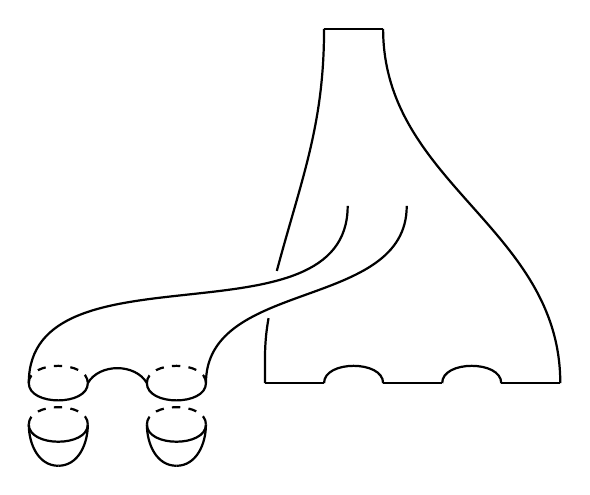
\begin{tikzpicture}[scale=1.5]
    \tikzset{->-/.style={decoration={ markings,
                mark=at position #1 with {\arrow{>}}},postaction={decorate}}}
    \draw [black, thick=1.5] (2,3) to[in=75,out=270] (1.6,0.95);
     \draw [black, thick=1.5] (1.53,0.55) to[in=90,out=260] (1.5,0); 
        
    \draw [black, thick=1.5] (2,0) to[in=90,out=90] (2.5,0);         
    \draw [black, thick=1.5] (3,0) to[in=90,out=90] (3.5,0);         
        \draw [black, thick=1.5] (2.5,3) to[in=90,out=270] (4,0);
    \draw [black, thick=1 ] (1.5,0) to (2,0); 
    \draw [black, thick=1 ] (2.5,0) to (3,0); 
    \draw [black, thick=1 ] (3.5,0) to (4,0); 
    \draw [black, thick=1] (2,3) to (2.5,3); 

    \draw [black, thick=1.5] (2.2,1.5) to[in=90,out=270] (-0.5,0);
    \draw [black, thick=1.5] (2.7,1.5) to[in=90,out=270] (1,0);
     \draw [black, thick=1.5] (0.5,0) to[in=60,out=120] (0,0); 

    \draw [black, thick=1.5, dashed] (-0.5,0) to[in=90,out=90] (0,0); 
    \draw [black, thick=1.5] (-0.5,0) to[in=270,out=270] (0,0); 
    \draw [black, thick=1.5, dashed] (0.5,0) to[in=90,out=90] (1,0); 
        \draw [black, thick=1.5] (0.5,0) to[in=270,out=270] (1,0); 

    \draw [black, thick=1.5, dashed] (-0.5,-0.35) to[in=90,out=90] (0,-0.35); 
    \draw [black, thick=1.5] (-0.5,-0.35) to[in=270,out=270] (0,-0.35); 
    \draw [black, thick=1.5, dashed] (0.5,-0.35) to[in=90,out=90] (1,-0.35); 
        \draw [black, thick=1.5] (0.5,-0.35) to[in=270,out=270] (1,-0.35); 

    \draw [black, thick=1.5] (-0.5,-0.35) to[in=180,out=270] (-0.25,-0.7); 
    \draw [black, thick=1.5] (0,-0.35) to[in=0,out=270] (-0.25,-0.7); 
  \draw [black, thick=1.5] (0.5,-0.35) to[in=180,out=270] (0.75,-0.7); 
    \draw [black, thick=1.5] (1,-0.35) to[in=0,out=270] (0.75,-0.7); 

\end{tikzpicture}
    \caption{Anchored disks}
    \label{anchored}
\end{figure}


Consider a system of parallel copies $\bar L=\{L_j\}_{j=0}^{\infty}$, where $L_0=L$, as in Section \ref{sec:parallel}. 
We first discuss numberings that determine the boundary conditions of our holomorphic disks.
Let $D_{m}$ denote the unit disk in the complex plane with $m$ boundary punctures
$\zeta_{1},\dots,\zeta_{m}$. One of the boundary punctures is distinguished. We choose notation so
that $\zeta_{1}$ is distinguished. The $m$ punctures subdivides the boundary of $D_{m}$ into $m$
boundary arcs. We will consider disks with numbered boundary arcs where the numbers correspond to
the parallel copies $L_{j}$. We will consider two types of numberings \emph{increasing} and
\emph{decreasing}: traversing the boundary of the disk in the positive direction starting from the
distinguished puncture, the numbering increases or remain constant respectively decreases or remain constant as we pass the other punctures. We call punctures where the numbering changes non-constant and punctures where it does not change constant. If the boundary numbering has no constant puncture then we call it strictly increasing or strictly decreasing. 

We next consider asymptotic conditions at the boundary punctures. There are two basic forms of asymptotics, a puncture is either asymptotic to a Lagrangian intersection point or to a Reeb chord. The former case is the standard form of asymptotics on Lagrangian Floer theory and the latter in Legendrian DG-algebras. More precisely, we choose an almost complex structure on $X$ which in the cylindrical end $\R\times Y$ is invariant under $\R$-translation, leaves the contact planes invariant and is compatible with the symplectic form induced on the contact planes by the contact form. Furthermore, it pairs the $\R$-direction with the Reeb direction. This means in particular that the Reeb chord strip which is the product of a Reeb chord and $\R$ is holomorphic and we study holomorphic disks with boundary punctures that are asymptotic to these Reeb chord solutions. 

Consider a disk $D_{m}$ as above with strictly increasing or decreasing numbering $\kappa=(\kappa_1,\dots,\kappa_{m})$ and let $\mathbf{a}=a_{1}\dots a_{m}$ be a word of Reeb chords and Lagrangian intersection points in $L_{0}\cap L_1$. We let $\mathcal{M}^{\fl}(\mathbf{a};\kappa)$ denote the moduli space of holomorphic disks $u\colon (D_{m},\partial D_{m})\to (X,\bar L)$ that satisfies the following conditions:
\begin{itemize}
\item $u$ takes the boundary component labeled by $\kappa_{j}$ to the Lagrangian $L_{\kappa_j}$.
\item $u$ is asymptotic to the unique Reeb chord or Lagrangian intersection point of $L_{\kappa_j}$ and $L_{\kappa_{j+1}}$ near $a_{j}$ at $\zeta_{j}$, where we let $\kappa_{m+1}=\kappa_{1}$.  	
\end{itemize} 


We next consider disks in the symplectization.  
Consider again the disk $D_{m}$ with boundary numbering $\kappa$ and punctures $\zeta_{1},\dots,\zeta_{m}$.  We next note that in the symplectization there are two possible Reeb chord asymptotics, positive or negative according to the sign of the $t$-coordinate near the puncture. Let $\mathbf{c}=c_{1}^{\sigma_{1}}\dots c_{m}^{\sigma_{m}}$ be a word of signed Reeb chords of $\Lambda_{0}\cup \Lambda_1$, where $\sigma\in\{+,-\}$ is a sign. 
If $m>1$ then we require that the Reeb chords $c_{r}$ at all constant punctures connect $\Lambda_{0}$ to $\Lambda_{0}$ and that their signs are all negative, $\sigma_{r}=-1$. We let $\mathcal{M}^{\sy}(\mathbf{c};\kappa)$ denote the moduli space of holomorphic disks $v\colon (D_{m},\partial D_{m})\to (\R\times Y,\R\times \Lambda)$ that satisfy the following conditions:
\begin{itemize}
	\item $v$ takes the boundary components labeled by $\kappa_{j}$ to the Lagrangian $\Lambda_{\kappa_j}$.
	\item $v$ is asymptotic at positive or negative infinity according to the sign of $\sigma_{j}$ to the unique Reeb chord between $\Lambda_{\kappa_j}$ and $\Lambda_{\kappa_{j+1}}$ near $c_{j}$ at a puncture $\zeta_{j}$.  		 
\end{itemize} 
We write $\mathcal{M}^{\sy}(\mathbf{c};\kappa)$ for the moduli space of holomorphic disks $v$ satisfying these conditions.

Finally, we consider disks in the cobordism and in the filled cobordism. We start with the cobordism
disks without filling. Consider a system of parallel copies $\bar C=\{C_{j}\}_{j=0}^{\infty}$.
Consider the disk $D_{i+j+2}$ where we fix two punctures that subdivide the boundary of the disk
into two arcs, upper and lower. Let $\kappa$ be a decreasing boundary numbering of the boundary
components in the upper arc and extend it to a constant numbering in the lower arc. Let
$\mathbf{c}_{0}=c_{0;1}\dots c_{0;j}$ be a composable word of Reeb chords connecting $\Lambda_{v}$
to $\Lambda_{w}$, and let $\mathbf{c}'=c_{i}\dots c_{1}$ be a word of Reeb chords of $\Gamma$. Consider the word of Reeb chords and intersection points 
\[ 
\mathbf{c}=c_{0;1}\dots c_{0;j}z^{w}c_{i}\dots c_{1}z^{v}
\]
and let 
\[ 
\mathcal{M}^{\co}(\mathbf{c};\kappa)
\]
denote the moduli space of holomorphic disks $u\colon (D_{i+j+2},\partial D_{i+j+2})\to (W,\bar C\cup L)$ such that the following holds.
\begin{itemize}
	\item $u$ is asymptotic to the Reeb chord $c_{0;r}$ at its $r^{\rm th}$ constant puncture, takes adjacent boundary arcs to $L$, and neighboring punctures to the unique intersection point near $z^{w}$ in $L\cap C^{w}_{\kappa_{i}}$ and near $z^{v}$ in $L\cap C^{v}_{\kappa_{i}}$, respectively. 
	\item On remaining boundary arcs and punctures the boundary maps as described by $\mathbf{c}$ and the numbering $\kappa$, exactly as above.
\end{itemize}

The disks in the filled cobordism are entirely analogous. Here we assume that $L$ is a Lagrangian submanifold in $X=X_{0}\cup W$. Consider again a system of parallel copies $\bar C=\{C_{j}\}_{j=0}^{\infty}$ and also a system of parallel copies $\bar L=\{L_{j}\}_{j=0}^{\infty}$ of $L$. Consider the disk $D_{i+j+2}$ where we fix two punctures that subdivide the boundary of the disk into two arcs, upper and lower. Let $\kappa$ be a decreasing boundary numbering of the boundary components in the upper and lower arcs. Let $\mathbf{x}_{0}=x_{0;1}\dots x_{0;j}$ be a word of intersection points of $L$ and let $\mathbf{c}'=c_{i}\dots c_{1}$ be a word of Reeb chords of $\Gamma$. Consider the word of Reeb chords and intersection points 
\[ 
\mathbf{c}=x_{0;1}\dots x_{0;j}z^{w}c_{i}\dots c_{1}z^{v}
\]
and let 
\[ 
\mathcal{M}^{\overline{\co}}(\mathbf{c};\kappa)
\]
denote the moduli space of holomorphic disks $u\colon (D_{i+j+2},\partial D_{i+j+2})\to (X,\bar C\cup \bar L)$ such that the following holds.
\begin{itemize}
	\item $u$ is asymptotic to the Reeb chord $x_{0;r}$ at its $r^{\rm th}$ puncture in the lower arc, takes adjacent boundary arcs to $L$, and neighboring punctures to the unique intersection point near $z^{w}$ in $L_{\kappa_{j}}^{w}\cap C^{w}_{\kappa_{j+1}}$ and the unique intersection point near $z^{v}$ in $K_{\kappa_{1}}\cap C^{v}_{\kappa_{i+j}}$. 
	\item On remaining boundary arcs and punctures the boundary maps as described by $\mathbf{c}$ and the numbering $\kappa$, exactly as above.
\end{itemize}



The formal dimension of the moduli spaces above is computed in terms of the negative of a Conley-Zehnder index $\mathrm{CZ}$ of the Reeb chords. Recall $\mathrm{CZ}(a)$ of a Reeb chord $a$ of $\Lambda$ as defined for example in \cite[Section 2.1]{BEE}: we pick paths connecting base points in the boundary of the various components of $L$, and paths connecting Reeb chord endpoints to the base points. We define $\mathrm{CZ}(a)$ to be the Maslov index of this path closed up by a positive rotation in the contact plane, and the grading $|a|=-\mathrm{CZ}(a)$. For a Lagrangian intersection $x$ between $L^{1}$ and $L^{2}$ we similarly pick paths connecting to the base points and use these to form a loop $\gamma$ starting in $L^{2}$ and ending in $L^{1}$ and define $\mathrm{CZ}(x)$ to be the Maslov index of the loop of Lagrangian planes that results from closing up the path of Lagrangian planes along $\gamma$ by a positive rotation, and $|x|=-\mathrm{CZ}(x)$. 

\begin{rem}
The above gradings are related to the grading $|\cdot|_{\mathrm{Leg}}$ in the Legendrian contact homology algebra, see e.g. \cite{EESPxR,BEE} as follows: 
\[ 
|c|_{\mathrm{Leg}}=-|c|-1.
\]
\end{rem} 
 
\begin{lem}
The formal dimension of the moduli space $\mathcal{M}^{\fl}(\mathbf{a};\kappa)$ equals
\[ 
\dim\left(\mathcal{M}^{\fl}(\mathbf{a};\kappa)\right)=
(n-3) - \sum_{j=1}^{m}(|a_{j}|-(n-2)).
\]
The formal dimension of the moduli space $\mathcal{M}^{\sy}(\mathbf{c};\kappa)$ equals
\[ 
\dim\left(\mathcal{M}^{\sy}(\mathbf{c};\kappa)\right)=
(n-3) + \sum_{\sigma_{j}=-1} (|c_{j}|+1) - \sum_{\sigma_{j}=+1}(|c_{j}|-(n-2)).
\]
The formal dimension of the moduli space $\mathcal{M}^{\co}(\mathbf{c};\kappa)$ equals
\[ 
\dim\left(\mathcal{M}^{\co}(\mathbf{c};\kappa)\right)=
1 - \sum_{r=1^{i}}(|c_{r}|-(n-2)) + \sum_{s=1}^{j} (|c_{0;s}|+1).
\]
The formal dimension of the moduli space $\mathcal{M}^{\overline{\co}}(\mathbf{c};\kappa)$ equals
\[ 
\dim\left(\mathcal{M}^{\overline{\co}}(\mathbf{c};\kappa)\right)=
1 - \sum_{r=1^{i}}(|c_{r}|-(n-2)) - \sum_{s=1}^{j} (|x_{0;s}|-(n-2)).
\]
\end{lem}

\begin{proof}
See \cite[Theorem A.1]{CEL}.
\end{proof}


We next study topological properties of the moduli spaces just defined. It turns out to be comparatively simple because of two key features. First, since we require our disks to switch copies at punctures ``in the same direction'' they cannot be multiply covered, and second, for the same reason there can be no boundary splitting. As in \cite{Ersft}, the first property allows us to prove transversality by perturbing the almost complex structure and the second shows that the moduli spaces admit compactifications consisting only of punctured curves joined at Reeb chords. Precise formulations of these results are as follows. 

\begin{thm}\label{thm:mdlitv}
For generic almost complex structure $J$ the moduli spaces $\mathcal{M}^{\fl}(\mathbf{a};\kappa)$, $\mathcal{M}^{\sy}(\mathbf{c};\kappa)$, $\mathcal{M}^{\co}(\mathbf{c};\kappa)$, and $\mathcal{M}^{\overline{\co}}(\mathbf{c};\kappa)$ are transversely cut out manifolds of dimensions $\dim(\mathcal{M}^{\fl}(\mathbf{a};\kappa))$ and $\dim(\mathcal{M}^{\sy}(\mathrm{c});\kappa)$, $\dim(\mathcal{M}^{\co}(\mathrm{c});\kappa)$, and $\dim(\mathcal{M}^{\overline{\co}}(\mathrm{c});\kappa)$, respectively. 
\end{thm}  

\begin{proof} To see this we note first that if $u$ is a disk in one of the moduli spaces then it
    cannot be multiply covered. We use the argument of \cite{EESPxR}. Fix a puncture of $u$.
    Consider first the more difficult case when this puncture maps to a Lagrangian intersection.
    Pick coordinates so that the intersection point lies at the origin in $\Cc^{n}$ and so that the
    two Lagrangians correspond to $\R^{n}$ and $i\R^{n}$. Let $(x_{1}+iy_{1},\dots,x_{n}+iy_{n})$ be
    standard coordinates on $\Cc^{n}$. Consider the complex hyperplanes
    $H_{\pm\epsilon}=\{x_{1}+iy_{1}=\pm\epsilon(1+i),x_{2}+iy_{2}=\dots=x_{n}+iy_{n}=0\}$. Looking
    at the Fourier expansion of $u$ near the puncture it is clear that for suitable coordinates
    (such that the leading Fourier coefficient of $u$ lies in direction of the first coordinate) the
    number of intersection points of the image of $u$ and $H_{\pm\epsilon}$ near the puncture have
    different parities depending on the sign of $\epsilon$. By analytic continuation, other disks
    and half disks mapping there either have images agreeing completely in the ball or there are
    injective points of the disk near the puncture. In the case where they agree completely we note
    that the parity of the number of intersection points in each local sheet not containing the
    puncture with $H_{\pm\epsilon}$ is independent of sign. We the find that we can achieve
    transversality by perturbing the complex structure near $H_{\pm\epsilon}$: because the sheet
    with the puncture intersects only one of $H_{\pm\epsilon}$, if the contributions of the sheets
    mapping to $H_{\epsilon}$ cancel then those mapping to $H_{\epsilon}$ cannot cancel and vice
    versa, by unique continuation.  \end{proof}

\begin{thm}\label{thm:mdlicmpct}
The moduli space $\mathcal{M}^{\fl}(\mathbf{a};\kappa)$ admits a compactification consisting of several level disks joined at Reeb chords and intersection points, where some levels may lie in the symplectization.

The moduli space $\mathcal{M}^{\sy}(\mathbf{c};\kappa)$ admits a compactification consisting of several level disks joined at Reeb chords. 

The moduli space $\mathcal{M}^{\co}(\mathbf{a};\kappa)$ admits a compactification consisting of several level disks joined at Reeb chords. There is one level of disks in the cobordisms and remaining levels in the symplectization ends.

The moduli space $\mathcal{M}^{\overline{\co}}(\mathbf{a};\kappa)$ admits a compactification consisting of several level disks joined at Reeb chords and intersection points. 

\end{thm}

\begin{proof}
Note that the boundary condition on our punctured disks have the following property: any arc that subdivides the source into two components with a positive puncture in each must connect boundary components numbered with distinct numbers. This shows that there can be no boundary splitting. The theorem then follows from SFT compactness \cite{BEHWZ}.
\end{proof}

We next discuss orientations of moduli spaces following \cite{EESori}. We fix capping operators at
all Reeb chords and Lagrangian intersection points so that the two capping operators there glue to a
disk with the Fukaya orientation, see \cite{FOOO}. Recall the relative spin structure on the Lagrangian submanifold induces an orientation on the determinant bundle over the space of disks with boundary condition in the Lagrangian, see. As in \cite{EESori} we see that these choices then induces a system of coherent orientations on the moduli spaces.


We will use one more property of the moduli spaces which says that they are effectively independent of the increasing or decreasing boundary labeling $\kappa$.

\begin{thm}\label{thm:mdlicopies}
Let $\kappa$ and $\kappa'$ be two increasing (decreasing) boundary numberings. Then there are canonical orientation preserving diffeomorphisms 
\begin{align*}
\mathcal{M}^{\fl}(\mathbf{a};\kappa)&\approx \mathcal{M}^{\fl}(\mathbf{a};\kappa'),\\
\mathcal{M}^{\sy}(\mathbf{c};\kappa)&\approx \mathcal{M}^{\sy}(\mathbf{c};\kappa'),\\
\mathcal{M}^{\co}(\mathbf{c};\kappa)&\approx \mathcal{M}^{\co}(\mathbf{c};\kappa')
\end{align*}
\end{thm}

\begin{proof}
Let $\mathcal{M}(\kappa)$ denote either one of the above moduli spaces. This moduli space is the transverse zero set of a Fredholm section in a Banach bundle. Changing the numbering from $\kappa$ to $\kappa'$ corresponds to an arbitrarily small isotopy which induces an arbitrarily small deformation of the section. The theorem follows. 
\end{proof}






\section{Wrapped Floer cohomology and Legendrian surgery}
In this section we outline an argument that establishes the isomorphism between
$CE^{\ast}(\Lambda)$ and $CW^*(C)$ where $C$ is the co-core disk of the surgery. Our proof is a
generalization of the corresponding result under Lagrangian handle attachment exposed in \cite{BEE}.
Since the description there is rather brief we discuss the basic steps also in the original case here. More precisely, we first
define a version of wrapped Floer cohomology using only purely holomorphic disks and show that the
resulting theory agrees with the usual version defined in terms of holomorphic disks with a
Hamiltonian term. Second we discuss the surgery isomorphism in \cite{BEE}, and third we discuss how
to generalize that argument to partially wrapped Floer cohomology calculations.

\subsection{Wrapped Floer cohomology  without Hamiltonian}\label{sec:CWnoHam}
Let $X$ be a Weinstein manifold and $L$ be an exact Lagrangian. Fix a system of shifting Morse functions that are positive at infinity and let $\bar L=\{L_{j}\}_{j=0}^{\infty}$ be the corresponding family of parallel
Lagrangian submanifolds. Define $CW^*(L)$ to be the chain complex generated by Reeb chords of $L$
and intersection points $L_{0}\cap L_{1}$. We define operations $\m_{i}$ on $CW^*(L)$ using what we call \emph{partial holomorphic buildings}.

We start in the simplest case when the output of $\m_{i}$ is an intersection point $c_{0}$. Consider
$i$ generators $c_{i}\dots c_{1}$ and consider a disk $D_{i+1}$ with a decreasing boundary numbering
$\kappa$, distinguished negative (output) puncture and remaining punctures positive (inputs). Let $\mathbf{c}'=c_{i}\dots c_{1}$ and $\mathbf{c}=c_{0}c_{i}\dots c_{1}$. Define
\[ 
\m_{i}'(\mathbf{c}') = \sum_{|c_{0}|=|\mathbf{c}'|+(2-i)}|\mathcal{M}^{\co}(\mathbf{c})|c_{0}.
\]
Here we use the temporary notion $\m_{i}'$ to denote the summand of the full operation $\m_{i}$ that takes values in intersection points. We next turn to the more complicated definition of the part $\m_{i}''$ of the operation that takes values in Reeb chord generators and to this end we introduce the notion of a partial holomorphic building.

The domain of partial holomorphic building is a possibly broken disk $D_{i+1}$ with decreasing
boundary numbering $\kappa$. The partial holomorphic buildings we consider always have exactly one
disk in the symplectization. We call it the primary disk of the building. We require that the
distinguished puncture which is increasing is a negative puncture of this primary disk. If the
distinguished puncture is the only negative puncture of the primary disk  then the partial building
consist only of its primary component. If on the other hand the primary disk has additional negative
punctures then we require that at each additional puncture (which is decreasing or constant) is a
disk in the cobordism with decreasing boundary condition is attached at its distinguished increasing
or constant puncture to the additional negative puncture. We call these disks the secondary disks of
the partial building. The resulting partial holomorphic building is then a disk with domain a broken
$D_{i+1}$, with distinguished puncture a negative puncture at a Reeb chord and with remaining $i$
punctures either Reeb chords or intersection points. See Figure \ref{partial}.

\begin{figure}[h!]
    \centering
    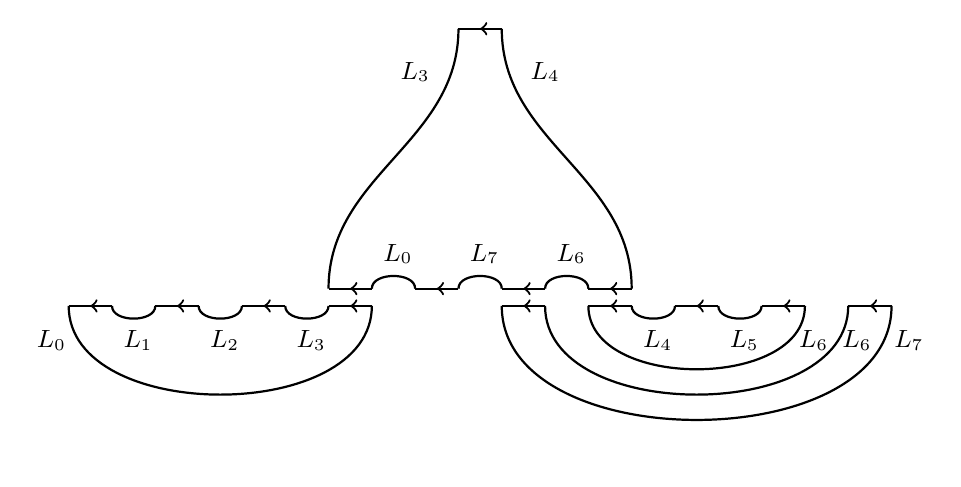
\begin{tikzpicture}[scale=1.1]
    \tikzset{->-/.style={decoration={ markings,
                mark=at position #1 with {\arrow{>}}},postaction={decorate}}}
    
    \draw [black, thick=1.5] (2,3) to[in=90,out=270] (0.5,0); 
    \draw [black, thick=1.5] (2.5,3) to[in=90,out=270] (4,0);
 
    \draw [black, thick=1.5] (2,0) to[in=90,out=90] (2.5,0);         
    \draw [black, thick=1.5] (3,0) to[in=90,out=90] (3.5,0);         
    \draw [black, thick=1.5] (1,0) to[in=90,out=90] (1.5,0);         
    
    \draw [black, thick=1.5] (0.5,-0.2) to[in=270,out=270] (0,-0.2);         
  \draw [black, thick=1.5] (-0.5,-0.2) to[in=270,out=270] (-1,-0.2);         
  \draw [black, thick=1.5] (-1.5,-0.2) to[in=270,out=270] (-2,-0.2);         
 
  \draw [black, thick=1.5] (5,-0.2) to[in=270,out=270] (5.5,-0.2);         
  \draw [black, thick=1.5] (4,-0.2) to[in=270,out=270] (4.5,-0.2);         
 


    \draw [black, thick=1.5] (1,-0.2) to[in=270,out=270] (-2.5,-0.2);         
 
    \draw [black, thick=1.5] (3.5,-0.2) to[in=270,out=270] (6,-0.2);         
     \draw [black, thick=1.5] (3,-0.2) to[in=270,out=270] (6.5,-0.2);         
 

    \draw [black, thick=1.5] (2.5,-0.2) to[in=270,out=270] (7,-0.2);         
 


    \draw [black, thick=1,->-=.5 ] (-2,-0.2) to (-2.5,-0.2); 
    \draw [black, thick=1,->-=.5 ] (-1,-0.2) to (-1.5,-0.2); 
    \draw [black, thick=1,->-=.5 ] (0,-0.2) to (-0.5,-0.2); 
    \draw [black, thick=1,->-=.5 ] (1,-0.2) to (0.5,-0.2); 
    \draw [black, thick=1, ->-=.5] (1,0) to (0.5,0); 
    \draw [black, thick=1, ->-=.5 ] (2,0) to (1.5,0); 
    \draw [black, thick=1, ->-=.5 ] (3,0) to (2.5,0); 
    \draw [black, thick=1, ->-=.5 ] (4,0) to (3.5,0); 
    \draw [black, thick=1, ->-=.5 ] (3,-0.2) to (2.5,-0.2); 
    \draw [black, thick=1, ->-=.5 ] (4,-0.2) to (3.5,-0.2); 
     \draw [black, thick=1, ->-=.5 ] (5,-0.2) to (4.5,-0.2); 
    \draw [black, thick=1,->-=.5 ] (6,-0.2) to (5.5,-0.2); 
    \draw [black, thick=1,->-=.5 ] (7,-0.2) to (6.5,-0.2); 
    \draw [black, thick=1,->-=.5] (2.5,3) to (2,3); 


 \node at (1.5,2.5) {\small $L_3$}; 
    \node at (3,2.5) {\small $L_4$}; 
    \node at (1.3, 0.4) {\small $L_0$}; 
    \node at (2.3, 0.4) {\small $L_7$}; 
    \node at (3.3, 0.4) {\small $L_6$}; 
     \node at (4.3, -0.6) {\small $L_4$}; 
     \node at (5.3, -0.6) {\small $L_5$};         
    \node at (6.1, -0.6) {\small $L_6$};         
    \node at (6.6, -0.6) {\small $L_6$};         
    \node at (7.2, -0.6) {\small $L_7$};         
    \node at (0.3, -0.6) {\small $L_3$}; 
  \node at (-0.7, -0.6) {\small $L_2$}; 
  \node at (-1.7, -0.6) {\small $L_1$}; 
  \node at (-2.7, -0.6) {\small $L_0$}; 



\end{tikzpicture}
    \caption{The domain of a partial building contributing to the operation $\m_7$ of $CW^*(L)$
    with a possible decoration. The map sends the tensor product of chords $L_0 \leftarrow L_1,
    L_1 \leftarrow L_2, \ldots, L_6 \leftarrow L_7$ to a chord $L_0 \leftarrow
    L_7$.} \label{partial}
\end{figure}

\begin{rem}
At additional negative punctures there may be constant holomorphic disks with one positive puncture and boundary on $L$ are attached. These are the usual augmentation disks, or disks on $L$ used as anchoring disks, compare Section \ref{ssec:parallelcopies}.   
\end{rem}
We write the punctures of the partial holomorphic disk building as $\mathbf{c}=c_{0}c_{i}\dots c_{1}$, where $c_{0}$ is the distinguished puncture. Write 
\[ 
\mathcal{M}^{\pb}(\mathbf{c};\kappa)
\]
for the moduli space of partial holomorphic disk buildings with boundary condition on $\bar L$ according to $\kappa$. Using this we define for generators $\mathbf{c}'=c_{i}\dots c_{1}$ the operation
\[ 
\m_{i}''(\mathbf{c}')=\sum_{|c_{0}|=|\mathbf{c}'|-(2-i)}|\mathcal{M}^{\pb}(\mathbf{c};\kappa)|c_{0},
\]
where the sum ranges over Reeb chords $c_{0}$ with grading as indicated. Finally we define the total operation $\m_{i}$ as the sum
\[ 
\m_{i}(\mathbf{c}')=\m_{i}'(\mathbf{c}') + \m_{i}''(\mathbf{c}').
\]


\begin{lem}
The $A_{\infty}$-relations hold for the operations $\m_i$.
\end{lem}
\begin{proof}
First, Theorem \ref{thm:mdlicopies} shows that the operations compose and that they are independent of the choice of decreasing boundary numbering. To see that the relations hold we will as usual identify the terms contributing to them with the boundary of an oriented 1-dimensional compact manifold. 

To this end we first consider 1-dimensional moduli spaces $\mathcal{M}'$ of the form    	
$\mathcal{M}'=\mathcal{M}^{\fl}(\mathbf{c};\kappa)$, where the distinguished puncture $c_{0}$ is an intersection point. As usual, the boundary numbering precludes boundary bubbling and we find that the boundary consists of broken disk that either break at an intersection point in which case the holomorphic parts both have dimension zero, or break into a partial holomorphic building with a rigid disk attached at its negative puncture, in which case the primary component of the partial building has dimension one. We find the boundary points of $\mathcal{M}'$ are in 1-1 correspondence with disks contributing to compositions of $\m_{i}'$ and $\m_{j}'$ (disks breaking at intersection points) and
disks contributing to $\m_{i}''$ and $\m_{j}'$. 

Remaining contributions to the $A_{\infty}$-relations correspond to compositions of $\m_{i}''$ and $\m_{j}''$. We identify also these with the boundary of an oriented 1-manifold. To this end we consider the boundary of the moduli space $\mathcal{M}''=\mathcal{M}^{\sy}(\mathbf{b};\kappa)$ of dimension two with distinguished negative puncture. (After we divide out the natural $\R$-action this is 1-dimensional space.) The boundary consists of two level broken disks and completing all negative punctures except the distinguished puncture with rigid disks in $\mathcal{M}^{\co}(\mathbf{a})$ we find also the composition of $\m_{i}''$ and $\m_{j}''$ expressed as the boundary of an oriented compact 1-manifold. The lemma follows.
\end{proof}

\subsubsection{Isomorphism with the Hamiltonian version}\label{sec:wrappediso}
We next show that the above definition of wrapped Floer cohomology agrees with the standard theory.
We keep the geometric setting as above and write $CW^{\ast}_{\mathrm{Ham}}(L)$ for the usual version
of Hamiltonian wrapped Floer cohomology. A well known argument \cite{EKH} shows that that
$CW^{\ast}(L)$ with differential $\m_{1}$ is quasi-isomorphic to the wrapped Floer cohomology by a
geometrically defined chain map. We extend this chain map to an $A_{\infty}$-map which then a standard spectral sequence argument establishes the desired isomorphism. 

We follow the approach in \cite{EO} where similar isomorphisms between contact and
symplectic differential graded algebras were constructed. More precisely, as there we
construct a splitting compatible non-negative field of $1$-forms with values in Hamiltonian vector
fields, and further a $1$-parameter family of such forms interpolating between the zero Hamiltonian
at the positive end and the Hamiltonian used to define wrapped Floer cohomology at the negative end, see \cite[Section 2]{EO}. We then define the corresponding moduli spaces over the deformation interval. Keeping the notation from \cite{EO} we denote them
\[ 
\mathcal{F}_{\R}(\mathbf{a},b).
\]

In order for the asymptotics at infinity of these maps to make sense we need to include the
parallel copies of the Lagrangians according to boundary numbering, and in particular also to
incorporate this in the description of wrapped Floer cohomology. More precisely, as in the case above we will have moduli spaces of Floer holomorphic disks with boundary in distinct Lagrangians that are arbitrarily close. The analogue of Theorem \ref{thm:mdlicopies} holds by the same argument and the corresponding moduli spaces are canonically isomorphic for sufficiently small perturbations. Using these observations we then define $\Phi\colon CW^{\ast}(L)\to CW^{\ast}_{\mathrm{Ham}}(L)$ by
\[ 
\Phi(\mathbf{a})=\sum_{\dim(\mathcal{F}_{\R}(\mathbf{a},b))=0}|\mathcal{F}_{\R}(\mathbf{a},b)|b.
\]
\begin{lem}
The map $\Phi$ is an $A_{\infty}$ homomorphism.
\end{lem}

\begin{proof}
To see this we note again that the disks which contributes to the $A_{\infty}$ relations correspond exactly to the ends of 1-dimensional moduli space.
\end{proof}

\begin{lem}
The map $\Phi$ is a quasi-isomorphism.
\end{lem}

\begin{proof}
The map respects the word length filtration and is the standard isomorphism from the linearized Legendrian cohomology to the wrapped Floer cohomology on the $E_2$-page.
\end{proof}


\subsection{Wrapped Floer cohomology and Lagrangian handle attachment}\label{ssec:CWBEE}
In this subsection we discuss the result in \cite{BEE} which gives a Legendrian surgery description of the wrapped Floer cohomology of a co-core disk in a Weinstein manifold obtained by Lagrangian handle attachment along a Legendrian sphere. To state this result we first introduce notation. 

Let $X_0$ be a Weinstein $2n$-manifold with ideal boundary the contact $(2n-1)$-manifold $Y_0$. Let $\Lambda=\Lambda_0\cup\dots\cup\Lambda_m$ be a Legendrian submanifold such that all of its components $\Lambda_j$ are parameterized $(n-1)$-spheres. Let $X$ be the Weinstein manifold that results from attaching Lagrangian handles $H$ to $\Lambda$. Here $H=H_{1}\cup\dots\cup H_{m}$, where each component $H_j$ is a disk sub-bundle of the cotangent bundle $T^{\ast}D$ of the $n$-disk $D$, and where $H_j$ is attached to $\Lambda_j$. Then $X$ contains $m$ co-core disks corresponding to the cotangent fibers at the center of the disk in each $H_j$. We let $C_j\subset X$ denote co-core disk in $H_j$, $\Gamma_j\subset Y$ denote its Legendrian boundary inside the contact boundary $Y$ of $X$, and write $\Gamma=\Gamma_1\cup\dots\cup\Gamma_m$. 

As a first step in the calculation of the wrapped Floer cohomology of $C$ we describe the generators of the underlying chain complex. By the results in Section \ref{sec:CWnoHam}, generators of $CW^{\ast}(C)$ are of two kinds Lagrangian intersection points and Reeb chords. Here the Lagrangian intersection points are easily understood: pick the shifting Morse function so that it has one minimum on each component of $C$ and no other critical points, then there is exactly one intersection point for each component of $C$. We denote the intersection point of $C_{j}$ by $m_{j}$ and we denote the subcomplex generated by the $m_{j}$ by $CW^{\ast}_{0}(\Gamma)$. Remaining generators are Reeb chords of $\Gamma$ we write $CW^{\ast}_{+}(\Gamma)$ for the quotient complex $CW^{\ast}(\Gamma)/CW^{\ast}_{0}(\Gamma)$ and note that $CW^{\ast}_{+}$ is generated by Reeb chords.
 
Consider the link $\Lambda$ and let all components be decorated by minus, $\Lambda^{-}=\Lambda$.
Consider $CE^{\ast}(\Lambda)$ as a chain complex, generated by composable words
of Reeb chords with differential $d$ and with product $\cdot$ given by concatenation if the words are composable and zero otherwise. Let $\epsilon>0$ denote the size of the attaching region (i.e., the size of the tubular neighborhood of $\Lambda$ where $H$ is attached), we then have the following.

\begin{lem}\label{l:BEEchords=words}
For any $A>0$ there exists $\epsilon_0>0$ such that if $\epsilon<\epsilon_0$ then there is a natural
    one to one correspondence between the generators of $CW_{+}^{\ast}(\Gamma)$ of action $<A$ and
    the generators of $CE^{\ast}(\Lambda)$ of action $<A$. 
\end{lem}

{\bf Sketch of proof:}  It is clear that a Reeb chord connecting $\Gamma_i$ to $\Gamma_j$ converges to a composable word of Reeb chords,
\[ 
\Lambda_{i}\to\Lambda\to\dots\to\Lambda\to\Lambda_{j},
\]
as $\epsilon\to 0$. To construct a unique chord for each composable word for small handles of size $\epsilon>0$ one uses an explicit model of the handle centered around the origin in standard symplectic $2n$-space where the Reeb flow corresponds to the solution of a linear differential equation in combination with an elementary finite dimensional fixed point theorem. Details will appear in \cite{BEEfuture}.

%Let $A(\Lambda)$ denote the chain complex generated by composable words, where a word $w$ is graded by $|w|+1$, where we include one empty word $e_i$ for each component $\Lambda_i$. We define a degree $-1$ product $\mu_2$ on $A(\Lambda)$ by concatenation, when the result is a composable word and zero when the concatenation is not composable. In particular, for empty words $e_ie_j=\delta_{ij}e_i$, where $\delta_{ij}$ is the Kronecker delta. The Legendrian co-algebra differential which counts holomorphic disks with one positive and several negative boundary punctures induces a degree $-1$ differential $\mu_1\colon A(\Lambda)\to A(\Lambda)$.

We will next define the surgery map which is an $A_{\infty}$-morphism
\[ 
\Phi\colon CW^{\ast}(\Gamma)\to CE^{\ast}(\Lambda),
\]
that counts certain holomorphic disks. See Figure \ref{surgerymap}.


\begin{figure}[h!]
    \centering
    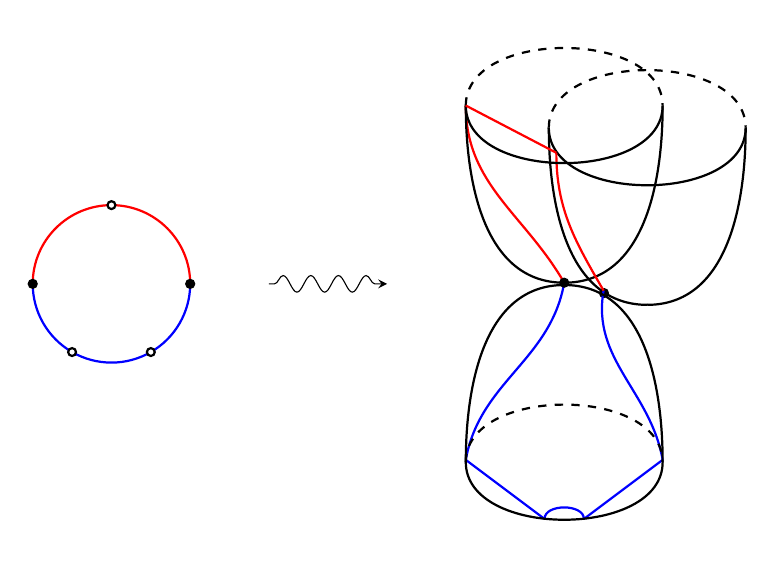
\begin{tikzpicture}[scale=1]
    \tikzset{->-/.style={decoration={ markings,
                mark=at position #1 with {\arrow{>}}},postaction={decorate}}}

        \draw[thick, red] (-1,0) arc (0:90:1);
        \draw[thick, red] (-2,1) arc (90:180:1);
        \draw[thick, blue] (-3,0) arc (180:240:1);
        \draw[thick, blue] (-2.5,{-sin(60)} ) arc (240:300:1);
        \draw[thick, blue] (-1.5,{-sin(60)} ) arc (300:360:1);

           \draw[thick, fill=white] (-2,1) circle(.05);
        \draw[thick, fill=white] (-1.5, {-sin(60)} ) circle(.05); 
        \draw[thick, fill=white] (-2.5, {-sin(60)} ) circle(.05); 
  

        \draw[thick, fill=black] (-1,0) circle(.05);
        \draw[thick, fill=black] (-3,0) circle(.05);


     \begin{scope}[xshift=30, yshift=92]
        \draw [black, thick=1.5, dashed, scale=5] (0.5,-0.25) to[in=90,out=90] (1,-0.25); 
        \draw [black, thick=1.5, scale=5] (0.5,-0.25) to[in=270,out=270] (1,-0.25); 

        \draw [black, thick=1.5, scale=5] (0.5,-0.25) to[in=180,out=270] (0.75,-0.7); 
        \draw [black, thick=1.5, scale=5] (1,-0.25) to[in=0,out=270] (0.75,-0.7); 
       
       \draw[thick, fill=black, scale=5] (0.64,-0.67) circle(.01);


     \end{scope}

    \begin{scope}[yshift=100]
     
          \draw[red, thick=1, scale=5] (0.5,-0.25) to[in=120,out=270] (0.75, -0.7); 


       \draw[blue, thick=1, scale=5] (0.5,-1.15) to (0.7, -1.3); 
      \draw[blue, thick=1, scale=5] (0.8,-1.3) to (1, -1.15); 
     
        \draw[blue, thick=1, scale=5] (1,-1.15) to[in=260,out=100] (0.85, -0.72); 
        \draw[blue, thick=1, scale=5] (0.5,-1.15) to[in=260,out=80] (0.75, -0.7); 
      \draw[blue, thick=1, scale=5] (0.7,-1.3) to[in=90,out=90] (0.8, -1.3);

 \draw [black, thick=1.5, scale=5] (0.5,-0.25) to[in=180,out=270] (0.75,-0.7); 
        \draw [black, thick=1.5, scale=5] (1,-0.25) to[in=0,out=270] (0.75,-0.7); 
        
         \draw[thick, fill=black, scale=5] (0.75,-0.7) circle(.01);


        
        \draw[red, thick=1, scale=5] (0.73,-0.37) to[in=120,out=270] (0.85, -0.72); 


            
            \draw [black, thick=1.5, dashed, scale=5] (0.5,-0.25) to[in=90,out=90] (1,-0.25); 
        \draw [black, thick=1.5, scale=5] (0.5,-0.25) to[in=270,out=270] (1,-0.25); 

             \draw[red, thick=1, scale=5] (0.5,-0.25) to (0.73, -0.37); 
         
    \end{scope}



        \begin{scope}[yscale=-1, yshift=100] 
            \draw [black, thick=1.5, scale=5] (0.5,-0.25) to[in=90,out=90] (1,-0.25); 
        \draw [black, thick=1.5, dashed, scale=5] (0.5,-0.25) to[in=270,out=270] (1,-0.25); 

        \draw [black, thick=1.5, scale=5] (0.5,-0.25) to[in=180,out=270] (0.75,-0.7); 
        \draw [black, thick=1.5, scale=5] (1,-0.25) to[in=0,out=270] (0.75,-0.7); 
        
        
              
        \end{scope}

    \draw[-stealth,decorate,decoration={snake,amplitude=3pt,pre length=2pt,post length=3pt}]
    (0,0.0) -- ++(1.5,0);


    \end{tikzpicture}
    \caption{A picture illustrating a curve contributing to $\Phi^1$ of
    the $A_\infty$ functor $\Phi$}
    \label{surgerymap}
\end{figure}

As in Section \ref{sec:mdlispaces}, consider the disk $D_{i+j+2}$ with two special punctures subdividing the boundary into an upper and a lower arc with $i$ and $j$ punctures respectively, and with a boundary numbering in the upper arc.  
Let $\mathbf{c}_{0}=c_{0;1}\dots c_{0;j}$ be a composable word of Reeb chords connecting
$\Lambda_{v}$ to $\Lambda_{w}$, and let $c_{i}\dots c_{1}$ be a word of generators of $CW^{\ast}(C)$. Consider the word of Reeb chords and intersection points 
\[ 
\mathbf{c}=c_{0;1}\dots c_{0;j}z^{w}c_{i}\dots c_{1}z^{v}.
\]

Define $\Phi_{i}\colon CW^{\ast}(C)^{\otimes_{i}}\to CE^{\ast}(\Lambda)$, 
\[ 
\Phi_i(\mathbf{c}')=\sum_{|\mathbf{c}_{0}|=|\mathbf{c}'|+i(n-2)}
|\mathcal{M}^{\co}(\mathbf{c})|\mathbf{c}_{0}.
\]
\begin{rem}
Note that if $m^{v}$ is the minimum of the Morse function on $C^{v}$ as above then 
\[ 
\Phi_{1}(m^{v})=e_{v},
\]
because of the unique holomorphic disk corresponding to the flow line from the minimum to the intersection point between $C^{v}\cap L$, for the parallel copies this gives a triangle with corners at $m^{v}=C^{v}_{0}\cap C^{v}_{1}$, at $C^{v}_{0}\cap L$, and at $C^{v}_{1}\cap L$, and since there are no negative punctures the output is $e_{v}$. Also,
and if a word $\mathbf{c}'$ of generators of $CW^{\ast}(C)$ contains a generator $m^{v}$ and has length $i>1$ then 
\[ 
\Phi_{i}(\mathbf{c}')=0,
\]
as this corresponds to a holomorphic disk with a flow line from the minimum attached and such a configuration cannot be rigid unless the disk is constant.
\end{rem}

\begin{thm}\label{l:BEEdiagonal}
The maps $\Phi_i$ gives an $A_{\infty}$-map $CW^{\ast}(C)\to CE^{\ast}(\Lambda)$ which is an $A_{\infty}$ quasi-isomorphism.	
\end{thm}

{\bf Sketch of proof:} In order to see the $A_{\infty}$-relations we study the boundary of the moduli space $\mathcal{M}^{\ha}(\mathbf{c})$. As usual the boundary numbering guarantees that there is no boundary splitting on $C$. The boundary of the moduli space thus consists of the following configurations. 
\begin{itemize}
\item[$(i)$] Two level curves with one level in the cobordism and one in either symplectization end.
\item[$(ii)$] Curves which split at the intersection point $C\cap L$.
\end{itemize}
Splitting $(i)$ corresponds to the map followed by the operation $d$ in
    $CE^{\ast}(\Lambda)$. Splitting $(ii)$ corresponds to the tensor product of the map followed by the product operation $\cdot$ in
    $CE^{\ast}(\Lambda)$. The $A_{\infty}$-relations follow.  

To see that $\Phi$ is a quasi-isomorphism we show that $\Phi_{1}$ induces an isomorphism on homology by constructing algebraically one holomorphic disks interpolating between a Reeb chord of $\Gamma$ and the corresponding word of Reeb chords of $\Lambda$. The existence of such disks implies that the map $\Phi_{1}$ has a triangular matrix with respect to the action filtration and hence is a chain isomorphism, compare \cite[Section 6.2]{BEE}. 

To construct the required interpolating disks one starts from unique and uniformly transversely cut out such disks for single chord words obtained by a straightforward explicit geometric construction. Gluing such disks at their Lagrangian intersection punctures in $L\cap C$ and using small action to rule out all breakings except one, we find that there is algebraically one disk interpolating between a chord on $\Gamma$ and the corresponding word of chords of $\Lambda$, see \cite{BEEfuture}.
The map being an $A_{\infty}$-quasi-isomorphism then follows from the word length spectral sequence.

\begin{rem}
A complete proof of Theorem \ref{l:BEEdiagonal}	has not yet appeared. In cases when splitting at Reeb orbits can be neglected it is possible to fill in the details in the above outline with classical techniques. As mentioned above, in the general case one must employ abstract perturbations to control holomorphic planes of anchored disks. The details of the perturbation scheme will not affect the argument. 
\end{rem}

\begin{rem}
There is also an ``upside-down'' perspective on the surgery just described. Namely, one can start from
    the contact manifold $Y$ and produce the contact manifold $Y_{0}$ by doing so called
    $+1$-surgery on $\Gamma$. In complete analogy with the above one shows that Reeb chords on
    $\Lambda$ are in natural one to one correspondence with words of Reeb chords on $\Gamma$ and one
    can construct an upside down surgery map of $A_\infty$ co-algebras:
\[ 
\Bar CW^{\ast}(C) \to LC_{\ast}(\Lambda).
\]
A similar argument also shows that this map is a quasi-isomorphism. Alternatively, one can prove this from the original surgery map using only algebra as follows. First write $CE^{\ast}(\Lambda)=\Omega LC_{\ast}(\Lambda)$ then
\[ 
\Bar CW^{\ast}(C) \simeq \Bar \Omega LC_{\ast}(\Lambda) \simeq  LC_{\ast}(\Lambda),
\]
since $LC_{\ast}(\Lambda)$ is co-nilpotent, see Section \ref{ssec:barcobaradj}.
\end{rem}

\subsection{Legendrian surgery and stopped wrapping}\label{ssec:CWpwrap}
In this section we outline a surgery approach to the computation of wrapped Floer homology in a
Weinstein manifold $X$ with wrapping stopped by a Legendrian $\Lambda$ in its boundary. We will use
the following model for the ambient manifold. Fix a tubular neighborhood of $\Lambda$ in the contact
boundary $Y$ of $X$ and attach a disk-bundle neighborhood of the $0$-section in
$T^{\ast}([0,\infty)\times\Lambda)$ along the boundary
$T^{\ast}([0,\infty)\times\Lambda)|_{0\times\Lambda}$ just like in Lagrangian handle attachment. We
use a Liouville vector field on this domain that agrees with the standard Liouville vector field
pointing outwards along fibers in the cotangent bundle over $[T,\infty)\times\Lambda$ for some
$T>0$. Let the components of $\Lambda$ be denoted $\Lambda_{v}$, $v\in Q_{0}$. Fix a base point
$p_v \in\Lambda_v$ for each $v$. Let $C^{v;\tau}$ denote the cotangent fiber $T^{\ast}_{(p_{v},\tau)}([0,\infty)\times\Lambda)$. We will compute the wrapped Floer cohomology of $C^{\tau}=\bigcup_{v\in Q_{0}}C^{v;\tau}$ for sufficiently large $\tau$ using a surgery approach. 

We first consider the surgery map into the Chekanov-Eliashberg algebra with loop space coefficients.
Consider all components of $\Lambda$ decorated by a positive sign $\Lambda=\Lambda^{+}$ and consider $CE^{\ast}(\Lambda)$ which now involves, except for Reeb chords, also chains $C_{-\ast}(\Omega\Lambda)$ on the based loop space. We define an $A_{\infty}$- map
\[ 
\Phi\colon CW^{\ast}(C)\to CE^{\ast}(\Lambda),
\]
where $A_{\infty}$-structure on the left hand side is the standard DG-algebra structure induced by concatenation and the Pontryagin product.  
As in Section \ref{sec:mdlispaces}, consider a disk $D_{i+j+2}$ with two dividing punctures that subdivides the boundary into two arcs, lower and upper. Let the upper arc contain $i$ boundary punctures and is equipped with a decreasing boundary numbering $\kappa$ and the lower arc $j$ boundary punctures. Let $\mathbf{c}'=c_{i}\dots c_{1}$ be Reeb chords of $C$ and let $\mathbf{c}_{0}=c_{0;1}\dots c_{0;j}$ be Reeb chords of $\Lambda$. Let
\[ 
\mathbf{c}= c_{0;1}\dots c_{0;j} z^{v} c_{i}\dots c_{1}\dots z^{w}
\]  
and consider $\mathcal{M}^{\co}(\mathbf{c};\kappa)$, again as in Figure \ref{surgerymap}.

Theorems \ref{thm:mdlitv} and \ref{thm:mdlicmpct} show that this moduli space carries a fundamental
chain. We view this chain as parametrizing chains of paths in $\Lambda$ connecting the Reeb chord
endpoints in $\mathbf{c}_{0}$. We write $[\mathcal{M}^{\co}(\mathbf{c})]$ for the alternating word
of chains of loops and Reeb chords and view it as an element in $CE^{\ast}(\Lambda)$. Define the maps 
\[ 
\Psi_{i}\colon CW^{\ast}(C)^{\otimes_\k i}\to CE^{\ast}(\Lambda)
\]
as 
\[ 
\Psi_{i}(\mathbf{c}')=\sum_{\mathbf{c}_{0}}[\mathcal{M}^{\st}(\mathbf{c})].
\]   


\begin{thm}\label{t:newsurgeryAinfty}
The map $\Psi\colon CW^{\ast}(C)\to CE^{\ast}(\Lambda)$ is an $A_{\infty}$-map.
\end{thm}

\begin{proof}
To see that the $A_{\infty}$-relation holds we look at the boundary of the moduli space $\mathcal{M}^{\co}(\mathbf{c})$ of dimension $d$. The codimension one boundary consists of three splittings:
\begin{itemize}
	\item[$(i)$] A one-dimensional curve splits off in the positive symplectization end.
	\item[$(ii)$] A one-dimensional curve splits off at the negative end.
	\item[$(iii)$] Splitting at one of the intersection points $z^{v}$. 
\end{itemize}
In order for splittings of the form $(i)$ to contribute to the codimension one boundary of the moduli space the part of the holomorphic building in $W$ consists of rigid disks with only positive punctures attached at one puncture to a negative puncture of the disk in the positive end and a disk of dimension $d-1$ in $\mathcal{M}^{\co}(\mathbf{b})$ attached at the remaining negative puncture. Assembling the rigid disks and the one-dimensional disk we get a partial holomorphic disk building that contributes to the $A_{\infty}$-operations in $CW^{\ast}(L)$ followed by the map $\Psi$. Splittings of type $(ii)$ corresponds to the map $\Psi$ followed by the differential $\mu_{1}$ in $CE^{\ast}(\Lambda)$. Finally splittings of type $(iii)$ correspond to the map $\Psi$ followed by the product $\mu_{2}$ on $CE^{\ast}(\Lambda)$. We conclude that the terms contributing to $A_{\infty}$-relations express the codimension one boundary of $[\mathcal{M}^{\co}(\mathbf{c})]$ in two different ways and hence $\Psi$ is an $A_{\infty}$-map.
\end{proof}

We will use slight generalizations of the map $\Psi$ below. More precisely, if $p_{j}$, $j=1,\dots,m$ are points in $[0,\infty)\times\Lambda$ and if $F_{j}$ is the cotangent fiber at $p_{j}$ then we have a similar surgery map
\[ 
\Psi^{p_ip_j}\colon CW^{\ast}(F_{i},F_{j})\to  CE^{\ast}_{p_ip_j}(\Lambda),
\]
which counts holomorphic disks with a positive Reeb chord connecting $F_{i}$ to $F_{j}$, two
Lagrangian intersection punctures at $p_{i}$ and at $p_{j}$, and a word of chains of loops in
$\Lambda$ and Reeb chords of $\Lambda$ as output, and where $CE^{\ast}_{ij}$ is directly analogous
to $CE^{\ast}$ but where the first chain of loops is in a word is replaced by a chain of paths from
$p_{i}$ to the base point and the last is replaced by a chain of paths from the base point to $p_{j}$.
In this setup the counterpart of the second component $\Psi_{2}$ is
\begin{equation}\label{eq:morefibersmap}
\Psi^{p_ip_jp_k}\colon CW^{\ast}(F_{j},F_{k})\otimes CW^{\ast}(F_{i},F_{j})\to CE^{\ast}_{p_ip_k}(\Lambda),
\end{equation}
and counts disks with two positive punctures at Reeb chords and two Lagrangian intersection punctures at $p_{i}$ and $p_{k}$. The counterpart of the $A_{\infty}$-equations in this setup is then
\begin{equation}\label{eq:morefibersprod} 
d\circ\Psi^{p_ip_k}+ \Psi^{p_jp_k}\cdot\Psi^{p_i p_j} + \Psi^{p_ip_jp_k}\circ(1\otimes\mu_{1}+\mu_{1}\otimes 1) + \Psi^{p_ip_k}\circ\mu_{2}=0, 
\end{equation}
where $d$ is the differential on $CE^{\ast}_{ik}$ and where $\cdot$ is the (Pontryagin) product
$CE^{\ast}_{p_j p_k}\otimes CE^{\ast}_{p_i p_j}\to CE^{\ast}_{p_ip_k}$. The proofs of these statements are word by word repetitions of the proof of Theorem \ref{t:newsurgeryAinfty}.


We next sketch a proof that the map $\Psi$ in Theorem \ref{t:newsurgeryAinfty} is in fact a
quasi-isomorphism, or, in other words, that its first component $\Psi_{1}$ induces an isomorphism on
homology. We filter $CW^{\ast}(C)$ by
action of its Reeb chord generators. To get a corresponding filtration on $CE^{\ast}(\Lambda)$ we
use action on Reeb chords in combination with the energy on the loops. We start with a discussion of the energy of loops, following \cite{Milnor}.

Equip $\Lambda$ with a Riemannian metric and  $\Omega=\Omega(\Lambda)$ denote the space of based loops in $\Lambda$ with the supremum norm: for two loops $\gamma,\beta\colon[0,1]\to \Lambda$,
\[
d^{\ast}(\gamma,\beta)=\sup_{t\in[0,1]} \rho(\gamma(t),\beta(t)),
\] 
where $\rho$ is the metric on $\Lambda$ induced by the Riemannian structure. Then the metric topology on $\Omega$ agrees with the standard compact open topology. 

Let $\Omega'=\Omega'(\Lambda)$ denote the space of piecewise smooth paths with metric
\[
d(\gamma,\beta) = d^{\ast}(\gamma,\beta)+ \int_{0}^{1}\left(|\dot\gamma|-|\dot{\beta}|\right)^{2}dt,
\]
where $\dot{\gamma}$ denotes the derivative of $\gamma$. The natural inclusion $\Omega'\to\Omega$ is
a homotopy equivalence, \cite[Theorem 17.1]{Milnor}. We will use finite dimensional approximations
to study $\Omega'$. The energy of a piece-wise smooth loop in $\Lambda$ is
\[
E(\gamma)= \int_0^{1}| \dot\gamma|^{2} dt.
\]
For $c>0$, let $\Omega^{c}\subset\Omega'$ denote the subset of loops of energy $E<c$. The space
$\Omega^{c}$ can be approximated by piece-wise geodesic loops. More precisely, fixing a subdivision
$0=t_{0}< t_{1}<\dots< t_{m}=1$ of $[0,1]$ we consider the space $B^{c}$ of loops of energy $E<c$
that are geodesic on each interval $[t_{i},t_{i+1}]$. Then \cite[Lemma 16.1]{Milnor} shows that for
all sufficiently fine subdivisions $B^{c}$ is a finite dimensional manifold (a submanifold of the
product $\Lambda^{\times m}$ in a natural way). Moreover \cite[Theorem 16.2]{Milnor}, all critical points of
$E|_{\Omega^c}$ lie in $B^{c}$ which is a deformation retract of $\Omega^{c}$ and for generic metric $E|_{B^{c}}$ is a Morse function. 

With these preliminaries established we turn to the actual proof. 
The first step will be to describe the Reeb chords of $C^{\tau}$. Let $g$ be a Riemannian metric on $\Lambda$ as above and let $f\colon [0,\infty)\to \R$ be a positive function with $f(0)=1$, $f'(0)=-1$, and $f'(t)<0$ monotone increasing. Define the metric $h$ on $\Lambda\times\R$ by
\[ 
h= dt^{2} + f(t) g.
\]




Then if $x$ and $y$ are points in $\Lambda$ and $\gamma\colon[0,s]\to\Lambda$ is a geodesic with $\gamma(0)=x$ and $\gamma(s)=y$ then there is a unique geodesic $(\gamma(t),r(t))\in\Lambda\times[0,\infty)$ such that
\begin{itemize}
	\item $(\gamma(0),0)=(x,0)$ and $(\gamma(s),r(s))=(y,0)$;
	\item $r(t)$ is Morse with has a unique maximum at an interior point $t=t_{0}$. 
\end{itemize}  

Note that the Reeb flow in the unit disk bundle is the natural lift of the geodesic flow. Assume next as above that the metric $g$ on $\Lambda$ is generic in the sense that the length functional for curves connecting any two Reeb chord endpoints in $\Lambda$ has only Morse critical points. Concretely, this means that the index form of any geodesic connecting two Reeb chord endpoints is non-degenerate. As in Lemma \ref{l:BEEchords=words}, this allows us to control the Reeb chords of $C^{\tau}$ below a given action for all sufficiently thin handles. More precisely, let $\epsilon$ denote the size of the tubular neighborhood of $\Lambda$ in $Y$ where we attach $T^{\ast}(\Lambda\times [0,\infty))$ and we introduce the following notion of a geodesic-Reeb chord word. A \emph{geodesic-Reeb chord word} is a word
\[ 
\gamma_{1}c_{1}\gamma_{2}c_{2}\dots c_{m}\gamma_{m},
\] 
where $\gamma_{1}$ is a geodesic from one of the base points $p_{v}$ to the start point of the
Reeb chord $c_{1}$, where $\gamma_{2}$ is a geodesic from the endpoint of $c_{1}$ to the start point
of $c_{2}$, etc, until finally $\gamma_{m}$ is a geodesic from the endpoint of the Reeb chord
$c_{m}$ to one of the base points $p_w$. We define the action of a geodesic-Reeb chord word to be the sum of actions of its Reeb chords and the energies of its geodesics.


\begin{lem}\label{l:newchords=words}
	For any $A>0$ there exists $\epsilon_{0}>0$ and $\tau_{0}>0$ such that for any $\epsilon<\epsilon_{0}$ and any $\tau>\tau_{0}$ there is a natural one to one correspondence between Reeb chords of $C^{\tau}$ of action $<A$ and geodesic-Reeb chord words of $\Lambda$ of action $<A$.
\end{lem}

{\bf Sketch of proof:} The proof uses the transversality of the Reeb chords and of the geodesics. The basic observation is that the point in the normal fiber of $\Lambda$ where the Reeb flow hits determines the direction of the geodesic in $\Lambda\times[0,\infty)$. After introducing a concrete smoothing of corners the lemma then follows from the finite dimensional inverse function theorem. 


To show that $\Psi_{1}$ is a quasi-isomorphism we will show that it is represented by a triangular
matrix with ones on the diagonal with respect to the action/energy filtration. To this end we will
use the Morse theoretic finite dimensional model for the chain complex underlying the homology of the based loop space described above. In order to have $[\mathcal{M}^{\co}(\mathbf{c})]$ defined as a chain in this model we need to assure that the paths on the boundary of the holomorphic disk are sufficiently well behaved. We only sketch the construction. On holomorphic disk with unstable domains, we fix gauge using small spheres surrounding Reeb chord endpoint, compare \cite[Section A.2]{ES}. As in \cite[Section A.1]{ES} we use a configuration space for holomorphic curves consisting of maps with two derivatives in $L^{2}$. This means that the restriction to the boundary has $3/2$ derivatives in $L^{2}$ and in particular the projection to $\Lambda$ has bounded energy. Since the action of the positive puncture in a holomorphic disk contributing to the differential controls the norm of the solution it follows that we can use configuration spaces of bounded energy to study the disks in the differential: we approximate the boundary curves uniformly by a piecewise geodesic curve by introducing a uniformly bounded number of subdivision points and straight line homotopies in small charts. 

\begin{conj}\label{appconj}
The chain-map $\Psi_{1}\colon CW^{\ast}(C)\to CE^{\ast}(\Lambda)$ induces an isomorphism on homology. 
\end{conj}

{\bf Sketch of proof:} 
Consider a word of the form
\[ 
\gamma_{0}c_{1}\gamma_{1} c_{2}\dots c_{m}\gamma_{m},
\]
where $\gamma_{j}$ are geodesics in $\Lambda\times[0,\infty)$ and where $c_{j}$ are Reeb chords. We aim to construct algebraically one disk connecting the Reeb chord $a$ of $C$, corresponding to this word (see Lemma \ref{l:newchords=words}), to the word itself. We use an inductive argument and energy filtration. To start the argument we pick additional fiber disks $F_{c^{+}}$ and $F_{c_{-}}$ in $T^{\ast}(\Lambda\times[0,\infty))$ at $(c^{+},\epsilon)$ and $(c_{-},\epsilon)$ for very small $\epsilon>0$ near all Reeb chord end points $c_{+}$ and $c_{-}$ in $\Lambda$. We use the natural counterparts of the for mixed wrapped Floer homologies. For example, there is a straightforward analogue of Lemma \ref{l:newchords=words}: Reeb chord generators of $CW^{\ast}(F_{c^{+}},C)$ correspond before the surgery words of the form
\[
\gamma_{1}c_{1}\gamma_{2}\dots c_{m}\gamma_{m},
\]
where $\gamma$ is a geodesic connecting the base point of $F_{c^{+}}$ to the startpoint of $c_{1}$,
$\gamma_{2}$ from the endpoint of $c_{1}$ to the start point of $c_{2}$, etc. To start the argument
we note that it is straightforward to construct holomorphic strips corresponding to the short
geodesics starting at $F_{c^{-}}$ followed by the chord $c$ and then the short geodesic to
$F_{c^{+}}$ and to show that they are unique. This corresponds to a generator of
$CW^*(F_{c^{-}},F_{c^{+}})$. Likewise, it is immediate to construct the holomorphic disk connecting a
Reeb chord generator of $CW^*(F_{c^{+}},C)$ corresponding to a geodesic, and show that it is unique, compare Lemma \ref{l:BEEdiagonal}. 

We now use these two to construct algebraically one disk from the Reeb chord generator of $CW^{\ast}(F_{c_{-}},C)$ corresponding to the short geodesic, the chord $c$, and a geodesic connecting the endpoint of $c$ to the base point of $C$. To this end we consider the natural map
\[
    \Psi^{p_v c^{+}c^{-}}\colon CW^*(F_{c^{+}},C)\otimes CW^*(F_{c^{-}},F_{c^{+}})\to CE^{\ast}(\Lambda),
\] 
see \eqref{eq:morefibersprod}. For the two Reeb chords $a$ connecting $F_{c^{-}}$ to $F_{c^{+}}$
corresponding to the chord $c$ of $\Lambda$, and $b$ connecting $F_{c^{+}}$ to $C$ corresponding to
the geodesic we then have (with $p_{v}$ denoting the base point):
\begin{align*}
    &d(\Psi^{p_{v} c^+ c^-}(b,a))+ (\Psi^{p_{v}c^-}(b))\cdot (\Psi^{c^{+}c^{-}}(a))  \\ 
    &+  \Psi^{p_{v} c^-}(\m_{2}(b,a)) + (-1^{|a|-1} \Psi^{p_v c^{+} c^-}(\m_{1}(b),a)
    +\Psi^{p_v c^{+}c^{-} }(b,\m_{1}(a)) =0. 
\end{align*}
Here we know that the terms containing $\m_{1}$ and $d$ involves non-trivial holomorphic disks or Morse flows in the finite dimensional approximation and hence lowers action/energy by an amount bounded below by some $\delta>0$ which we assume is much larger than $\epsilon>0$ above. Therefore, if we restrict attention to a small action window we find
\[ (\Psi^{p_{v}c^- }(b) \cdot \Psi^{c^{+}c^{-}}(a))+\Psi^{p_{v} c^-}(\m_{2}(b,a))=0.
\]
Here the first term is simply the Pontryagin product at the common endpoint of the curves, which is
homologous to the word $\epsilon'c\gamma$ of the small geodesic, the Reeb chord and then the longer
geodesic, by rounding the corner at $c^{+}$. It follows that $\m_{2}(a,b)=r$, where $r$ is a Reeb
chord with action between the sum of the actions of $a$ and $b$ and the action of $\epsilon'c\gamma$
and that $\Psi^{c^{-}p_{v}}(r)$ contains this word with coefficient $\pm 1$. Noting that there
is only one Reeb chord in the action window studied we find that the desired coefficient equals $\pm
1$. It is now clear how to continue the induction, in each step we add one more geodesic or Reeb
chord to any word. Using already constructed curves and \eqref{eq:morefibersprod} in a small action
window we find that the map $\Psi_{1}$ has a triangular action matrix with $\pm 1$ on the diagonal,
hence it is a quasi-isomorphism. 








\end{document}
